\documentclass[12pt]{article}
\usepackage[usenames,dvipsnames]{color}
\usepackage{color}
\usepackage{amsmath,amsfonts,url,amssymb,graphicx,float,epstopdf,subfigure,subfig,color,tikz}
\usepackage{bigstrut}
\usepackage{array}
\usepackage{multirow}
\usepackage{amsthm}
\usepackage{fancyhdr}
\usepackage{url,amssymb,amsthm}
\usepackage{bm}
\usepackage{layout}
\usepackage{fancyhdr}
\usepackage{graphicx}
\usepackage{courier}
\usepackage{amsmath}
\usepackage{titlesec}
\usepackage{color}
\usepackage[usenames,dvipsnames]{color}
\usepackage{amsmath,amsfonts,url,amssymb,graphicx,float,epstopdf,subfigure,subfig,color}
\usepackage{bigstrut}
\usepackage{array}
\usepackage{multirow}
\usepackage{amsthm}
\usepackage{fancyhdr}
\usepackage{url,amssymb,amsthm}
\usepackage{bm}
\usepackage{layout}
\usepackage{fancyhdr}
\usepackage{graphicx}
\usepackage{courier}
\usepackage{amsmath}
\usepackage{titlesec}
\usepackage{color}
\usepackage[top=3cm, bottom=3cm, left=4cm, right=3cm]{geometry}
\usepackage{graphicx}
\usepackage{epstopdf}
\usepackage{multicol}

\makeatletter
% Increase oddsidemargin from 0.5in to 1.6cm
\oddsidemargin=1.6cm
\evensidemargin 0in
% Remove marginparwidth from 40pt to 0pt
\marginparwidth=0pt
% Remove marginparsep from 10pt to 0pt
\marginparsep=0pt
\topmargin 0pt
\headsep .5in
% Increase textheight from 8.1in to 9in
\textheight=8in
% Decrease textwidth from 6in to 5.75in
\textwidth=5.75in
% Move the entire page up by 0.4cm
\voffset=-0.4cm

%\setlength{\textheight}{20cm}
%\setlength{\voffset}{0.9cm}
%\setlength{\textwidth}{14cm}
%\setlength{\hoffset}{-0.26cm}
\pagestyle{fancy}
\fancyhead[RO, LE]{J. G. Smith}

\def\B{\rm{B\"ack\-lund }}
\def\P{Painlev\'e }
\def\w{Wronskian }
\def\ws{Wronskians }
\def\L{\mathcal{L}}
\def\J{\mathcal{J}}
\def\F{\mathcal{F}}
\def\K{\mathcal{K}}
\def\W{\mathcal{W}}

\def\Z{\mathbb{Z}}
\def\N{\mathbb{N}}
\def\R{\mathbb{R}}
\def\C{\mathbb{C}}
\def\efri{\rm{efri(z)}}
\def\erfc{\rm{efrc(z)}}

\def\e{e^{-z}}

\def\k{\kappa}\def\th{\vartheta}

\newtheorem{mydef}{Theorem}[section]
\newtheorem{mydef1}{Definition}[section]
\newtheorem{mydef2}{Proof}[section]
\newtheorem{mydef3}{Remark}[section]
\newtheorem{mydef4}{Corollary}[section]

\numberwithin{figure}{section}
\numberwithin{equation}{section}
\numberwithin{table}{section}

\renewcommand{\baselinestretch}{1.6}

\begin{document}

\begin{titlepage}
\title{\P Equations and Orthogonal Polynomials}
\author{James G. Smith\\ School of Mathematics, Statistics and Actuarial Science\\ University of Kent, Canterbury, CT2
7NF}
\date{}
\clearpage
\maketitle
\thispagestyle{empty}
\end{titlepage}
\newpage
\begin{abstract}
In this thesis we classify all of the special function solutions to \P equations and all their associated equations produced using their Hamiltonian structures. We then use these special solutions to highlight the connection between the \P equations and the coefficients of some three-term recurrence relations for some specific orthogonal polynomials. The key idea of this newly developed method is the recognition of certain orthogonal polynomial moments as a particular special function. This means we can compare the matrix of moments with the Wronskian solutions, which the \P equations are famous for. Once this connection is found we can simply read off the all important recurrence coefficients in a closed form. In certain cases, we can even improve upon this as some of the weights allow a simplification of the recurrence coefficients to polynomials and with it, the new sequences orthogonal polynomials are simplified too.
\end{abstract}
\newpage
\renewcommand{\abstractname}{Acknowledgements}
\begin{abstract}
This thesis is based on research carried out in the of School of Mathematics, Statistics and Actuarial Science at the University of Kent in the years $2011-2015$, funded by the EPSRC. I would like to thank everyone who made this possible.

I am very grateful to my supervisor Prof Peter Clarkson for introducing me to this fascinating subject. His experience, knowledge and expertise have played an integral part throughout my PhD.

I also owe many thanks to all the staff at the Kent School of Mathematics, Statistics and Actuarial Science. In particular, a member of the admin staff, Claire Carter was not only my first go to with any problem, but also an excellent friend throughout the highs and the lows and I feel I owe her a lot.

I must also give a particulary special mention to my office mates; Bill, Andrea, Su and An, who have been extremely tolerant of my overly active shenanigans and my sporadic descents into incomprehensibility. They have been there every step of the way and I am positive I have formed four friendships that will last a lifetime. Speaking of incomprehensibility; I, of course, need to mention my good friend Mark. Mark was able to provide not only intense mathematical discussions, but also equally intense, entirely essential escapism.

The last person I need to acknowledge has been a big part of my life for a number of years now and I owe her a huge debt for her moral support, her countless hours of grammar checking and her meticulous attention to detail with my spelling (which I insist wasn't necessary). Nethertheless, thank you Vicky. \#Soulmates.

\end{abstract}
\newpage
\renewcommand{\abstractname}{Declaration}
\begin{abstract}
I declare that this thesis was composed by myself and that the work contained therein is my own, except where explicitly stated otherwise.
\end{abstract}
\newpage

\tableofcontents
\newpage
\listoffigures
\newpage
\section{Introduction}
\subsection{General Introduction}
In this thesis we will discuss the following orthogonal polynomials: various deformed Laguerre polynomials, Pollaczek-Jacobi polynomials, time-dependent Jacobi polynomials, some polynomials on the unit circle and some deformed Jacobi polynomials. Once the logarithmic derivative of Hankel and \w determinants are taken it can be compared directly to one of the \P equations special function solutions \cite{Rec}. Our goal in this thesis is to explore a new method of computing the recurrence coefficients for specific orthogonal polynomial weights using the comparison we mentioned above.

Some of the solutions to the \P equations comprise of classical special functions, such as the Bessel functions, the Airy function, the Legendre functions and the confluent hypergeometric function. Recently \cite{P:PAC&KJ} there has been much interest in the relationship between semi-classical orthogonal polynomials and these integrable
equations. This relationship dates back to work by Shohat \cite{P:325:2251} in $1939$. It took until $1995$, in a paper by Magnus \cite{P:57:37}, to establish
that these integrable equations were actually \P equations. These relationships extend to many of the \P equations. For example, see
\cite{P:42:320,Basor,P:44:035202,Chen,Rec,P:PAC&KJ,P:45:205201,Ormerod,2004:159,Bornemann}. The purpose of this thesis is to explore and clarify this connection.

The thesis is organised into the following sections:
\begin{itemize}
\item Introduction to \P and all the material we will be using, including the vital Hamiltonian structures.
\item Introduction to the special function solutions and how they are related to the \P equations $P_{II} - P_{VI}$.
\item Introduce the idea of rational function solutions. Some of these solutions can be shown to be special cases of the special function solutions which we will see in more detail later.
\item The applications of the special function and rational function solutions and how they relate explicitly to certain orthogonal polynomials. This is chapters $5$, $6$, $7$ and $8$ of the thesis and contains most of the original work. We will be applying a new method to some previously known orthogonal polynomial weights.
\end{itemize}
\subsection{\P equations}

The six \P equations $(P_I - P_{VI})$ were first discovered approximately $100$ years ago by \P and his colleagues whilst investigating ordinary differential equations of the form
\begin{equation}\nonumber
\frac{d^2w}{dz^2}=F\bigg(z;w,\frac{dw}{dz}\bigg),
\end{equation}
where $F$ is rational in $\frac{dw}{dz}$ and $w$ is analytic in $z$. They possess the property that their solutions have no movable essential singularities. Alternatively, the locations of multi-valued singularities of any of the solutions are independent of the particular solutions chosen and so are dependent only on the equation.
This is now known to be the {\it\P property}. \P\hspace{-1mm}, Gambier and their colleagues managed to
show that there are $50$ canonical equations with this property up to a M\"obius (bilinear rational) transformation
$$
W(\zeta)=\frac{a(z)w+b(z)}{c(z)w+d(z)},~~~\zeta=\phi(z),
$$
where $a(z),$ $b(z)$, $c(z)$, $d(z)$ and $\phi(z)$ are locally analytic functions.
Contained inside these $50$ equations are the six \P equations. The remaining $44$ equations can either be reduced to linear equations and
solved in terms of elliptic functions, or can be reduced to ordinary differential equations satisfied by the transcendental solutions.  The solutions of $(P_I - P_{VI})$ are called the \P transcendents and the general solutions of the \P equations are transcendental. This means they are irreducible; they cannot be expressed in terms of previously known functions, such as rational functions, elliptic functions or special functions. The \P equations have a plethora of interesting properties, some of which will be investigated in this thesis. Some of these properties include:
\begin{itemize}
\item \B transformations. These transformations relate one solution (from within a hierarchy) to another solution.
\item Special function solutions (which are also known as one parameter solutions). \P equations can be thought of as nonlinear analogues of the classical special function solutions and these solutions play a vital role in this thesis.
\item Rational function solutions are found for $P_{II} - P_{VI}$ and are sometimes formed as a subset of the special function solutions. However, this is not the case for all \P equations. For example, $P_{IV}$ \eqref{PIV} has its rational function solutions formed as a subset of the special function solutions of $P_{VI}$ \eqref{PIV}. However, $P_{III}$ \eqref{PIII} has some rational solutions that cannot be produced from the special function solutions of $P_{III}$ \eqref{PIII}.
\item \P asymptotics. These leading order asymptotics are a useful way for determining (from an applied point of view) which equation a suspected exact \P solution belongs to and where exactly it appears in the hierarchy.
\end{itemize}
The \P equations arise in a large number of applications, for example; random matrix theory, the asymptotic theory of orthogonal polynomials,
self-similar solutions of integrable equations, tiling problems as well as many more \cite{P:1303.0773}.
The six Painlev\'{e} equations $(P_I - P_{VI})$ are the nonlinear ordinary differential equations defined below.
\begin{subequations}
\begin{align}
\!\frac{d^2w}{dz^2}&= 6w^2 + z,\label{PI}\\
\!\frac{d^2w}{dz^2}&= 2w^3 + zw + A,\label{PII}\\
\!\frac{d^2w}{dz^2}&=\frac{1}{w}\bigg(\frac{dw}{dz}\bigg)^2-\frac{1}{z}\frac{dw}{dz}+ \frac{{A}w^2 + B}{z}+{C}w^3 + \frac{D}{w},\label{PIII}\\
\!\frac{d^2w}{dz^2}&= \frac{1}{2w}\bigg(\frac{dw}{dz}\bigg)^2+\tfrac{3}{2}{w^3}+ 4zw^2+ 2(z^2-A)w+ \frac{B}{w},\label{PIV}\\
\!\frac{d^2w}{dz^2}&=\Bigg{(}\frac{1}{2w}+\frac{1}{w-1}\Bigg{)}\bigg(\frac{dw}{dz}\bigg)^2-\frac{1}{z}\frac{dw}{dz}+\frac{(w-1)^2}{z^2}\Bigg{(}{A}w+\frac{B}{w}\Bigg{)}\nonumber\\
&\qquad+\frac{{C}w}{z}+\frac{{D}w(w+1)}{w-1},\label{PV}\\
\!\frac{d^2w}{dz^2}&=\frac{1}{2}\Bigg{(}\frac{1}{w}\!+\!\frac{1}{w-1}\!+\!\frac{1}{w-z}\Bigg{)}{\bigg(\frac{dw}{dz}\bigg)^2}\!-\!\Bigg{(}\frac{1}{z}\!+\!\frac{1}{z-1}\!+\!\frac{1}{w-z}\Bigg{)}\frac{dw}{dz}\nonumber\\
&\qquad+\frac{w(w\!-\!1)(w\!-\!z)}{z^2(z-1)^2}\Bigg{\{}\!A\!+\!\frac{{B}z}{w^2}\!+\!\frac{{C}(z-1)}{(w-1)^2}\!+\!\frac{{D}z(z-1)}{(w-z)^2}\!\Bigg{\}}\label{PVI}.
\end{align}
\end{subequations}
where $A,B,C$ and $D$ are arbitrary constants.

\subsection{Hamiltonian structure}
Each \P equation has its own Hamiltonian structure and
system to explore. The \P system associated with $P_J$ is, by definition, the Hamiltonian system
\begin{equation}\label{HE}
\delta_Jq=\frac{\partial \mathcal{H}_J}{\partial p},~\delta_Jp=-\frac{\partial \mathcal{H}_J}{\partial q},
\end{equation}
where $\delta$ is the operator associated with that \P equation for a unique Hamiltonian function $\mathcal{H}_J$ \cite{P:13:47} and is given for each case by
\begin{align}
\delta&=\frac{d}{dz} &&\rm{for~~J=I,II,IV},\\
\delta&=z\frac{d}{dz} &&\rm{for~~J=III,V},\\
\delta&=z(z-1)\frac{d}{dz} &&\rm{for~~J=VI},
\end{align}
where the Hamiltonian functions $\mathcal{H}_J$ are given by
\begin{subequations}
\begin{align}
\mathcal{H}_{I}(q,p,z)&= \tfrac{1}{2}p^2-2q^3-zq,\label{HI}\\
\mathcal{H}_{II}(q,p,z)&= \tfrac{1}{2}p^2-(q^2+\tfrac{1}{2}z)p-(\alpha+\tfrac{1}{2})q,\label{HII}\\
\mathcal{H}_{III}(q,p,z)&= q^2p^2-zpq^2-(\lambda_0-1)pq+zp+\tfrac{1}{2}(\lambda_0-2-\lambda_{\infty})zq,\label{HIII}\\
\mathcal{H}_{IV}(q,p,z)&=2qp^2-(q^2+2zq+2\kappa_0)p+\kappa_{\infty}q,\label{HIV}\\
\mathcal{H}_{V}(q,p,z)&=q(q-1)^2p^2-\{(\beta+\vartheta)q^2-(2\beta+\vartheta-z)q+\beta\}p\nonumber\\
   &\qquad-\tfrac{1}{4}\{\alpha^2-(\beta+\vartheta)^2\}q,\label{HV}\\
\mathcal{H}_{VI}(q,p,z)&=q(q-1)(q-z)p^2-\big\{\th_4(q-1)(q-z)+\th_3q(q-z)\nonumber\\
   &\qquad+(\th_0-1)q(q-1)\big\}p+\th_2(\th_1+\th_2)(q-z),\label{HVI}
\end{align}
\end{subequations}
where $\alpha,\beta,\vartheta,\th_0,\th_1,\th_2,\th_3,\th_4,\th_\infty,\lambda_0,\lambda_\infty,\kappa_0$ and $\kappa_\infty$ are arbitrary constants.
To elaborate, the function $\sigma_n=\mathcal{H}_J+L(z)$ where $L(z)$ is a linear correction term will satisfy a non-linear second-order, second-degree ordinary differential equation (ODE), often referred to as the \P $\sigma$-equation.

It is also interesting to note that $P_{V}$ \eqref{PV} has the option of using either the delta operator as $\delta=\frac{d}{dz}$ or $\delta=z\frac{d}{dz}$. We will discuss this unique feature of $P_{V}$ \eqref{PV} in chapter $2$.
\begin{mydef3}
Each Hamiltonian function $\sigma=H_J$ satisfies a second-order second-degree
ordinary differential equation whose solutions are in a correspondence
with solutions of the associated \P equation through \eqref{HE} since
$$q=F_J\bigg(\sigma,\frac{d\sigma}{dz},\frac{d^2\sigma}{dz^2},z\bigg),~~~p=G_J\bigg(\sigma,\frac{d\sigma}{dz},\frac{d^2\sigma}{dz^2},z\bigg),$$
for suitable functions $F_J\big(\sigma,\frac{d\sigma}{dz},\frac{d^2\sigma}{dz^2},z\big)$ and $G_J\big(\sigma,\frac{d\sigma}{dz},\frac{d^2\sigma}{dz^2},z\big)$. Thus, given $q$ and $p$, one can determine $\sigma$ and conversely, given $\sigma$, one can determine $q$ and $p$. This will be shown in detail later.
\end{mydef3}

The six Painlev\'{e} $\sigma$-equations $(S_I - S_{VI})$ are the nonlinear ordinary differential equations defined below:
\begin{subequations}
\begin{align}
&\bigg(\frac{d^2\sigma}{dz^2}\bigg)^2+4\bigg(\frac{d\sigma}{dz}\bigg)^3+2z\frac{d\sigma}{dz}-2\sigma=0,\label{SI}\\
&\bigg(\frac{d^2\sigma}{dz^2}\bigg)^2+4\bigg(\frac{d\sigma}{dz}\bigg)^3+2\frac{d\sigma}{dz}\bigg(z\frac{d\sigma}{dz}-\sigma\bigg)=\tfrac{1}{4}(\alpha+\tfrac{1}{2})^2,\label{SII}\\
&\bigg(z\frac{d^2\sigma}{dz^2}-\frac{d\sigma}{dz}\bigg)^2+4\bigg(\frac{d\sigma}{dz}\bigg)^2\bigg(z\frac{d\sigma}{dz}-2\sigma\bigg)+4z\th_\infty\frac{d\sigma}{dz}=z^2
\bigg(z\frac{d\sigma}{dz}-2\sigma+2\th_0\bigg),\label{SIII}\\
&\bigg(\frac{d^2\sigma}{dz^2}\bigg)^2-4\bigg(z\frac{d\sigma}{dz}-\sigma\bigg)+4\bigg(\frac{d\sigma}{dz}+2\th_0\bigg)\bigg(\frac{d\sigma}{dz}+2\th_\infty\bigg)=0,\label{SIV}\\
&\bigg(z\frac{d^2\sigma}{dz^2}\bigg)^2=\bigg[2\bigg(z\frac{d\sigma}{dz}\bigg)^2-z\frac{d\sigma}{dz}+\sigma\bigg]^2-4\prod_{j=0}^3\bigg(
\frac{d\sigma}{dz}+\kappa_j\bigg),\label{SV}\\
&\frac{d\sigma}{dz}\bigg(z(z-1)\frac{d^2\sigma}{dz^2}\bigg)^2+\bigg(\frac{d\sigma}{dz}\bigg\{2\sigma-(2z-1)\frac{d\sigma}{dz}\bigg\}+\kappa_1\kappa_2\kappa_3\kappa_4\bigg)^2
=\prod^4_{j=1}\bigg(\frac{d\sigma}{dz}+\kappa_j^2\bigg),\label{SVI}
\end{align}
\end{subequations}
where $\beta,\vartheta_0,\vartheta_\infty$ and $\kappa_0,...,\kappa_4$ are arbitrary constants.

In the following sections we will derive all of the $\sigma$-equations $(S_I - S_{VI})$ that we will need in this thesis. The Hamiltonian functions $\sigma = H_J$ frequently arise in applications, e.g:
random matrix theory and orthogonal polynomials. It is this connection with the orthogonal polynomial applications which make the derivations of each $\sigma$-equation fundamentally important. All of the calculation in the following section can be found on the USB flash drive in its appropriate folder.
\subsubsection{Hamiltonian structure for the first \P equation $P_{I}$}
The Hamiltonian associated with $P_{I}$ \eqref{PI} is
\begin{equation}
\mathcal{H}_{I}(q,p,z) = \tfrac{1}{2}p^2-2q^3-zq,\label{HI}
\end{equation}
where Hamilton's equations \eqref{HE} yield the following system, which $p$ and $q$ satisfy:
\begin{subequations}\label{HISYS}
\begin{align}
\frac{dq}{dz}=&p,\label{HI1}\\
\frac{dp}{dz}=&6q^2+z.\label{HI2}
\end{align}
\end{subequations}
Eliminating $p$ in \eqref{HI1} then $q=w$ satisfies $P_I$ \eqref{PI}.
\begin{mydef} The Hamiltonian function
\begin{equation}
\sigma(z)=\mathcal{H}_{I}(q,p,z),\label{HA1}
\end{equation}
with $\mathcal{H}_I(q,p,z)$ given by \eqref{HI}, satisfies the second-order, second-degree equation
$$
\bigg(\frac{d^2\sigma}{dz^2}\bigg)^2+4\bigg(\frac{d\sigma}{dz}\bigg)^3+2z\frac{d\sigma}{dz}-2\sigma=0,
$$
which is $S_{I}$ \eqref{SI}.
Conversely, if $\sigma(z)$ satisfies $S_I$ \eqref{SI} then the solutions of the Hamiltonian system \eqref{HISYS} are given by
\begin{equation}\label{PIpandq}
q(z)=-\sigma',\quad
p(z)=-\sigma'',\quad'=\frac{d}{dz}.
\end{equation}
\end{mydef}
\begin{proof}
Substituting \eqref{HI} into \eqref{HA1} and differentiating twice followed by substituting \eqref{HI1} and \eqref{HI2} where possible yields
\begin{subequations}
\begin{align}
\frac{d\sigma}{dz} &=-q,\label{SId1}\\
\frac{d^2\sigma}{dz^2} &=-p.\label{SId2}
\end{align}
\end{subequations}
Then, solving \eqref{SId1} and \eqref{SId2} simultaneously gives \eqref{PIpandq}.
Substituting \eqref{PIpandq} into $H_{I}$ \eqref{HI} we can generate $S_{I}$ \eqref{SI} multiplied by some other expression.
Also see Okamoto \cite{P:56:264,P:30:305} and Forrester and Witte \cite{P:57:679}.
\end{proof}
\subsubsection{Hamiltonian structure for the second \P equation  $P_{II}$}
The Hamiltonian associated with $P_{II}$ \eqref{PII} is the following:
\begin{equation}
\mathcal{H}_{II}(q,p,z) = \tfrac{1}{2}p^2-(q^2+\tfrac{1}{2}z)p-(\alpha+\tfrac{1}{2})q,\label{HII}
\end{equation}
where Hamilton's equations \eqref{HE} yield the following system, which $p$ and $q$ satisfy:
\begin{subequations}\label{HIISYS}
\begin{align}
\frac{dq}{dz}=&p-q^2-\tfrac{1}{2}z,\label{HII1}\\
\frac{dp}{dz}=&2qp+\alpha+\tfrac{1}{2}.\label{HII2}
\end{align}
\end{subequations}
Eliminating $p$ in \eqref{HII1} then $q=w$ satisfies $P_{II}$ \eqref{PII}. Whilst eliminating $q$ yields
\begin{equation}
p\frac{d^2p}{dz^2}=\tfrac{1}{2}\bigg(\frac{dp}{dz}\bigg)^2+2p^3-2p^2-\tfrac{1}{2}(\alpha+\tfrac{1}{2})^2,
\end{equation}
which is known as $P_{34}$.
\begin{mydef} The Hamiltonian function
\begin{equation}
\sigma(z)=\mathcal{H}_{II}(q,p,z),\label{HA2}
\end{equation}
with $\mathcal{H}_{II}(q,p,z)$ given by \eqref{HII}, satisfies a second-order, second-degree equation
$$
\bigg(\frac{d^2\sigma}{dz^2}\bigg)^2+4\bigg(\frac{d\sigma}{dz}\bigg)^3+2\frac{d\sigma}{dz}\bigg(z\frac{d\sigma}{dz}-\sigma\bigg)=\tfrac{1}{4}(\alpha+\tfrac{1}{2})^2,
$$
which is $S_{II}$ \eqref{SII}.
Conversely, if $\sigma(z;\alpha)$ satisfies $S_{II}$ \eqref{SII} then the solutions of the Hamiltonian system \eqref{HIISYS} are given by
\begin{equation}\label{PIIpandq}
q(z) =\frac{4\sigma''+2\alpha+1}{8\sigma'},\quad
p(z)=-2\sigma',\quad'=\frac{d}{dz}.
\end{equation}
\end{mydef}
\begin{proof}
Substituting \eqref{HII} into \eqref{HA2} and differentiating twice followed by substituting \eqref{HII1} and \eqref{HII2} where possible yields
\begin{subequations}
\begin{align}
\frac{d\sigma}{dz}&=-\tfrac{1}{2}p,\label{SIId1}\\
\frac{d^2\sigma}{dz^2}&=-qp-\tfrac{1}{2}\alpha-\tfrac{1}{4}.\label{SIId2}
\end{align}
\end{subequations}
Then, solving \eqref{SIId1} and \eqref{SIId2} simultaneously gives \eqref{PIIpandq}.
Substituting \eqref{PIIpandq} into $H_{II}$ \eqref{HII} we can generate $S_{II}$ \eqref{SII} multiplied by some other expression.
Also see Okamoto \cite{P:56:264,P:30:305} and Forrester and Witte \cite{P:57:679}.
\end{proof}
\subsubsection{Hamiltonian structure for the third \P equation $P_{III}$}
The Hamiltonian associated with $P_{III}$ \eqref{PIII} is the following:
\begin{equation}
\mathcal{H}_{III}(q,p,z) = q^2p^2-zpq^2-(\lambda_0-1)qp+zp+\tfrac{1}{2}(\lambda_0-2-\lambda_\infty)zq,\label{HIII}
\end{equation} with $\lambda_0$ and $\lambda_{\infty}$ parameters,
where Hamilton's equations \eqref{HE} yield the following system, which $p$ and $q$ satisfy:
\begin{subequations}\label{HIIISYS}
\begin{align}
z\frac{dq}{dz}&=2pq^2-zq^2-(\lambda_0-1)q+z,\label{HIII1}\\\label{HIII2}
z\frac{dp}{dz}&=-2qp^2+2zpq+(\lambda_0-1)p-\tfrac{1}{2}(\lambda_0-2-\lambda_\infty)z.
\end{align}
\end{subequations}
See Okamoto \cite{P:2:525,P:30:305}.
Eliminating $p$ in \eqref{HIII1} then $q=w$ satisfies $P_{III}$ \eqref{PIII}.
\begin{mydef} The Hamiltonian function
\begin{equation}
\sigma(z;\lambda_0,\lambda_\infty)=\tfrac{1}{2}\mathcal{H}_{III}(q,p,z)+\tfrac{1}{2}pq+\tfrac{1}{8}(\lambda_0-2)^2-\tfrac{1}{4}z^2,\label{HA3}
\end{equation}
with $\mathcal{H}_{III}(q,p,z)$ given by \eqref{HIII}, satisfies the second-order, second-degree equation
$$
\bigg(z\frac{d^2\sigma}{dz^2}-\frac{d\sigma}{dz}\bigg)^2+4\bigg(\frac{d\sigma}{dz}\bigg)^2\bigg(z\frac{d\sigma}{dz}-2\sigma\bigg)+4z\th_\infty\frac{d\sigma}{dz}=z^2
\bigg(z\frac{d\sigma}{dz}-2\sigma+2\th_0\bigg),
$$
which is $S_{III}$ \eqref{SIII} with the parameters
$$\{\th_0,\th_\infty\}=\{-\tfrac{1}{4}\lambda_\infty(\lambda_0-2),\tfrac{1}{8}(\lambda^2_\infty+(\lambda_0-2)^2)\}.$$
Conversely, if $\sigma(z;\lambda_0,\lambda_\infty)$ satisfies
$S_{III}$ \eqref{SIII} then the solutions of the Hamiltonian system \eqref{HIIISYS} are given by
\begin{equation}\label{PIIIpandq}
q(z)=\frac { 2z\sigma''+2(1-\lambda_0)\sigma'-\lambda_\infty z}{z^2-4(\sigma')^2},\quad
p(z)=\sigma'+\tfrac{1}{2}z,\quad'=\frac{d}{dz}.
\end{equation}
\end{mydef}
\begin{proof}
Substituting \eqref{HIII} into \eqref{HA3} and differentiating twice followed by substituting \eqref{HIII1} and \eqref{HIII2} where possible yields
\begin{subequations}
\begin{align}
\frac{d\sigma}{dz}&=p-\tfrac{1}{2}z,\label{SIIId1}\\
\frac{d^2\sigma}{dz^2}&=\frac{1}{2z}(4qp(z-p)+2p\lambda_0-z(\lambda_0-\lambda_\infty-1)-2p).\label{SIIId2}
\end{align}
\end{subequations}
Then, solving \eqref{SIIId1} and \eqref{SIIId2} simultaneously gives \eqref{PIIIpandq}.
Substituting \eqref{PIIIpandq} into $H_{III}$ \eqref{HIII} we can generate $S_{III}$ \eqref{SIII} multiplied by some other expression.
Also see Okamoto \cite{P:56:367,P:30:305} and Forrester and Witte \cite{P:57:679}.
\end{proof}
\subsubsection{Hamiltonian structure for the third \P equation $P_{III'}$}
An alternative form of $P_{III}$ \eqref{PIII}, due to Okamoto \cite{P:56:264,P:56:367,P:30:305}, is obtained by making the transformation $w(z)=u(t)/\sqrt t$, with $t=\tfrac{1}{4}z^2$ in $P_{III}$ \eqref{PIII} giving
\begin{equation}
\frac{d^2u}{dt^2}=\frac{1}{u}{\bigg(\frac{du}{dt}\bigg)\!}^2-\frac{1}{t}\frac{du}{dt}+\frac{u^2}{2t^2}(A+2u)+\frac{B}{2t}-\frac{1}{u},\label{PIIIi}
\end{equation}
which is well known to be $P_{III'}$ \eqref{PIIIi}.
The Hamiltonian associated with $P_{III'}$ \eqref{PIIIi} is the following:
\begin{equation}
\mathcal{H}_{III'}(q,p,t) = q^2p^2 -\left(q^2+\th_0q-t\right)p +\tfrac12(\th_0+\th_{\infty})q,\label{HIIIi}
\end{equation} with $\th_0$ and $\th_{\infty}$ parameters,
where Hamilton's equations \eqref{HE} yield the following system, which $p$ and $q$ satisfy:
\begin{subequations}\label{HIIIiSYS}
\begin{align}
t\frac{dq}{dt}&=2q^2p-q^2-\th_0q+t,\label{HIIIi1}\\\label{HIIIi2}
t\frac{dp}{dt}&=-2qp^2+2qp+\th_0p-\tfrac12(\th_0+\th_{\infty}).
\end{align}
\end{subequations}
See Okamoto \cite{P:56:264,P:56:367,P:30:305}.
Eliminating $p$ in \eqref{HIIIi1} then $q=w$ satisfies $P_{III}$ \eqref{PIII} with parameters  $(A,B)=(-2\th_{\infty},2(\th_0+1))$.
Eliminating $q$ in \eqref{HIIIi2} then $p$ satisfies
\begin{align}\nonumber
\frac{d^2p}{dt^2}&=\frac{1}{2}\bigg(\frac{1}{p}+\frac{1}{p-1}\bigg)\bigg(\frac{dp}{dt}\bigg)^2-\frac{1}{t}\frac{dp}{dt}-\frac{2p(p-1)}{t}\\
&\qquad+\frac{1}{8t^2}\bigg\{4\th_0\th_\infty-\frac{(\th_0+\th_\infty)^2}{p}-\frac{(\th_0-\th_\infty)^2}{p-1}\bigg\}.\label{PIIIdiff1}
\end{align}
Making the transformation $p(t)=1/[1-w(z)]$, with $z=t$ in \eqref{PIIIdiff1} yields
\begin{equation}\nonumber
\frac{d^2w}{dz^2}=\bigg(\frac{1}{2w}+\frac{1}{w-1}\bigg)\bigg(\frac{dw}{dz}\bigg)-\frac{1}{z}\frac{dw}{dz}+\frac{(w-1)^2}{z^2}\bigg\{\frac{(\th_0+\th_\infty)^2w}{8}
-\frac{(\th_0-\th_\infty)^2}{8w}\bigg\}-\frac{2w}{z},
\end{equation}
which is $P_V$ \eqref{PV} with parameters $$\{A,B,C,D\}=\{\tfrac{1}{8}(\th_0+\th_\infty)^2,-\tfrac{1}{8}(\th_0-\th_\infty)^2,-2,0\}.$$
This is precisely the well known connection between $P_{III}$ \eqref{PIIIi} and $P_V$ \eqref{PV} when $D=0$.
\begin{mydef} The Hamiltonian function
\begin{equation}
\sigma(z;\th_0,\th_\infty)=t\mathcal{H}_{III'}(q,p,t)-\tfrac{1}{2}t+\tfrac{1}{4}\th_0^2,\label{HA3i}
\end{equation}
with $\mathcal{H}_{III'}(q,p,z)$ given by \eqref{HIIIi} satisfies the second-order, second-degree equation
\begin{equation}
\bigg(t\frac{d^2\sigma}{dt^2}\bigg)^2+\bigg\{4\bigg(\frac{d\sigma}{dt}\bigg)^2-1\bigg\}\bigg(t\frac{d\sigma}{dt}-\sigma\bigg)+\th_0\th_\infty\frac{d\sigma}{dt}=\tfrac{1}{4}(\th_0^2+\th_\infty^2).\label{SIIIi}
\end{equation}
Conversely, if $\sigma(z;
\th_0,\th_\infty)$ satisfies $S_{III'}$ \eqref{SIIIi} then the solutions of the Hamiltonian system \eqref{HIIIiSYS} are given by
\begin{equation}\label{PIIIipandq}
q(t)=\frac { 2t\sigma''-2\th_0\sigma'+\th_\infty}{1-4(\sigma')^2},\quad
p(t)=\sigma'+\tfrac{1}{2},\quad'=\frac{d}{dt}.
\end{equation}
\end{mydef}
\begin{proof}
Substituting \eqref{HIIIi} into \eqref{HA3i} and differentiating twice followed by substituting \eqref{HIIIi1} and \eqref{HIIIi2} where possible yields
\begin{subequations}
\begin{align}
\frac{d\sigma}{dt}&=p-\tfrac{1}{2},\label{SIIIid1}\\
\frac{d^2\sigma}{dt^2}&=\frac{1}{2t}(4qp(1-p)+2\th_0p-\th_0-\th_\infty).\label{SIIIid2}
\end{align}
\end{subequations}
Then, solving \eqref{SIIIid1} and \eqref{SIIIid2} simultaneously gives \eqref{PIIIipandq}.
Substituting \eqref{PIIIipandq} into $H_{III'}$ \eqref{HIIIi} we can generate $S_{III'}$ \eqref{SIIIi} multiplied by some other expression.
Also see Okamoto \cite{P:56:367,P:30:305} and Forrester and Witte \cite{P:219:357}.
\end{proof}
\subsubsection{Hamiltonian structure for the fourth \P equation $P_{IV}$}
The Hamiltonian associated with $P_{IV}$ \eqref{PIV} is the following:
\begin{equation}
\mathcal{H}_{IV}(q,p,z)=2qp^2-(q^2+2zq+2\kappa_0)p+\kappa_{\infty}q,\label{HIV}
\end{equation}
with $\kappa_0$, $\kappa_{\infty}$ parameters, where Hamilton's equations \eqref{HE} yield the following system, which $p$ and $q$ satisfy:
\begin{subequations}\label{HIVSYS}
\begin{align}
\frac{dq}{dz}&=4qp-q^2-2zq-2\kappa_0,\label{HIV1}\\
\frac{dp}{dz}&=-2p^2+2pq+2zp-\kappa_{\infty}.\label{HIV2}
\end{align}
\end{subequations}
Eliminating $p$ then $q=w$ satisfies $P_{IV}$ \eqref{PIV} with the following parameters:
$\{A,B\}=\{1-\kappa_0+2\kappa_{\infty},-2\kappa_{0}^2\}$. Whilst eliminating $q$, then $w=-2p$ satisfies $P_{IV}$ \eqref{PIV} with the following parameters:
$\{A,B\}=\{2\kappa_0-\kappa_{\infty}-1,-2\kappa_{\infty}^2\}$.
As in the usual case for \P equations, this Hamiltonian equation satisfies a second-order, second-degree equation.
\begin{mydef} The Hamiltonian function
\begin{equation}
\sigma(z;\kappa_0,\kappa_\infty)=\mathcal{H}_{IV}(q,p,z),\label{HA4}
\end{equation}
with $\mathcal{H}_{IV}(q,p,z)$ given by \eqref{HIV} satisfies the second-order, second-degree equation
$$
\bigg(\frac{d^2\sigma}{dz^2}\bigg)^2-4\bigg(z\frac{d\sigma}{dz}-\sigma\bigg)+4\bigg(\frac{d\sigma}{dz}+2\th_0\bigg)\bigg(\frac{d\sigma}{dz}+2\th_\infty\bigg)=0,
$$
which is $S_{IV}$ \eqref{SIV} with the parameters
$$\{\th_0,\th_\infty\}=\{\kappa_0,\kappa_\infty\}.$$
Conversely, if $\sigma(z;\kappa_0,\kappa_\infty)$ satisfies $S_{IV}$ \eqref{SIV} then the solutions of the Hamiltonian system \eqref{HIVSYS} are given by
\begin{equation}\label{PIVpandq}
q(z)=\frac { \sigma''-2z\sigma'+2\sigma}{ 2(\sigma'+2\kappa_\infty)},\quad
p(z)={\frac { \sigma''+2z\sigma'-2\sigma }{ 4(\sigma'+2\kappa_0)}},\quad'=\frac{d}{dz}.
\end{equation}
\end{mydef}
\begin{proof}
Substituting \eqref{HIV} into \eqref{HA4} and differentiating twice followed by substituting \eqref{HIV1} and \eqref{HIV2} where possible yields
\begin{subequations}
\begin{align}
\frac{d\sigma}{dz}&=-2qp,\label{SIVd1}\\
\frac{d^2\sigma}{dz^2}&=-4qp^2+(4\kappa_0-2q^2)p+2\kappa_\infty q.\label{SIVd2}
\end{align}
\end{subequations}
Then, solving \eqref{HIV}, \eqref{SIVd1} and \eqref{SIVd2} simultaneously gives \eqref{PIVpandq}.
Substituting \eqref{PIVpandq} into $H_{IV}$ \eqref{HIV} we can generate $S_{IV}$ \eqref{SIV} multiplied by some other expression.
Also see Jimbo and Miwa \cite{P:2:407} and Okamoto \cite{P:275:221}.
\end{proof}
\subsubsection{Hamiltonian structure for the fifth \P equation  $P_{V}$}
The Hamiltonian associated with $P_{V}$ \eqref{PV} is the following:
\begin{equation}
\mathcal{H}_{V}(q,p,z)=q(q-1)^2p^2-\{(b+\vartheta)q^2-(2b+\vartheta-z)q+b\}p-\tfrac{1}{4}\{a^2-(b+\vartheta)^2\}q,\label{HV}
\end{equation}
with $a$, $b$ and $\vartheta$ as parameters and
where Hamilton's equations \eqref{HE} yield the following system, which $p$ and $q$ satisfy:
\begin{subequations}\label{HVSYS}
\begin{align}
z\frac{dq}{dz}&=2q(q-1)^2p-(b+\vartheta)q^2+(2b+\vartheta-z)q-b,\label{HV1}\\
z\frac{dp}{dz}&=-(3q-1)(q-1)p^2+2(b+\vartheta)qp-(2b+\vartheta-z)p+\tfrac{1}{4}\{a^2-(b+\vartheta)^2\}.\label{HV2}
\end{align}
\end{subequations}
\begin{proof}
See Jimbo and Miwa \cite{P:2:407} Okamoto \cite{P:56:264,P:56:367,P:13:47}.
\end{proof}
Eliminating $p$ then $q=w$ satisfies \eqref{PV} with the following parameters:
$\{A,B,C\}=\{\tfrac{1}{2}{a^2},-\tfrac{1}{2}{b^2},-\vartheta-1\}$.
As in the usual case for \P equations, this Hamiltonian equation satisfies a second-order, second-degree equation.
\begin{mydef} The Hamiltonian function
\begin{equation}
\sigma(z;a,b,\vartheta)=\mathcal{H}_V(q,p,z)+\tfrac{1}{4}(2b+\vartheta)z-\tfrac{1}{8}(2b+\vartheta)^2,\label{sigHv}
\end{equation}
with $\mathcal{H}_V(q,p,z)$ given by \eqref{HV}, satisfies the second-order, second-degree equation
$$
\bigg(z\frac{d^2\sigma}{dz^2}\bigg)^2=\bigg[2\bigg(z\frac{d\sigma}{dz}\bigg)^2-z\frac{d\sigma}{dz}+\sigma\bigg]^2-4\prod_{j=0}^3\bigg(
\frac{d\sigma}{dz}+\kappa_j\bigg),
$$
which is $S_{V}$ \eqref{SV} with the parameters
$$\{\kappa_0,\kappa_1,\kappa_2,\kappa_3\}=\big\{\tfrac{1}{4}(\vartheta+2a),\tfrac{1}{4}(\vartheta-2a),-\tfrac{1}{4}(\vartheta+2b),
\tfrac{1}{4}(2b-\vartheta)\big\}.$$
Conversely, if $\sigma(z;
a,b,\vartheta)$ satisfies \eqref{SV} then the solutions of the Hamiltonian system \eqref{HVSYS} are given by
\begin{equation}\label{PVpandq}
q(z) =\frac { z\sigma''+2(\sigma')^{2}-z\sigma' +\sigma}{ 2(\sigma'+\tfrac{1}{4}\vartheta-\tfrac12a) (\sigma'
+\tfrac{1}{4}\vartheta+\tfrac{1}{2}a)},\quad
p(z) ={\frac { z\sigma''-2(\sigma')^{2}+z\sigma'-\sigma }{ 2(\sigma'-\tfrac{1}{4}\vartheta+\tfrac{1}{2}b)}},\quad'=\frac{d}{dz}.
\end{equation}
\end{mydef}
\begin{proof}
Substituting \eqref{HV} into \eqref{sigHv} and differentiating twice followed by substituting \eqref{HV1} and \eqref{HV2} where possible yields
\begin{subequations}
\begin{align}
\frac{d\sigma}{dz}&=\tfrac{1}{4}(2b+\vartheta)-qp,\label{SVd1}\\
\frac{d^2\sigma}{dz^2}&=\frac{1}{z}(q^3p^2-(b+\vartheta)q^2p-(\tfrac{1}{4}(a+b+\vartheta)(a-b-\vartheta)+p^2)q+b p).\label{SVd2}
\end{align}
\end{subequations}
Solving \eqref{sigHv}, \eqref{SVd1} and \eqref{SVd2} simultaneously gives \eqref{PVpandq}.
Substituting \eqref{PVpandq} into $H_{V}$ \eqref{HV} we can generate $S_{V}$ \eqref{SV} multiplied by some other expression.
Also see Jimbo and Miwa \cite{P:2:407} and Okamoto \cite{P:56:367,P:30:305}.
\end{proof}
\subsubsection{Hamiltonian structure for the sixth \P equation  $P_{VI}$}
The Hamiltonian associated with $P_{VI}$ \eqref{PVI} is the following:
\begin{align}\nonumber
\mathcal{H}_{VI}(q,p,z)=&~q(q-1)(q-z)p^2-\big\{\th_4(q-1)(q-z)+\th_3q(q-z)\\&\qquad+(\th_0-1)q(q-1)\big\}p+\th_2(\th_1+\th_2)(q-z),\label{HVI}
\end{align}
where $\th_0$, $\th_1$,$\th_2$ and $\th_3$ are parameters and are related in the following way:
$$\th_0+\th_1+2\th_2+\th_3+\th_4=1,$$
where Hamilton's equations \eqref{HE} yield the following system, which $p$ and $q$ satisfy:
\begin{subequations}\label{HVISYS}
\begin{align}\nonumber
z(z-1)\frac{dq}{dz}&=-3{p}^{2}{q}^{2}+ \big\{( 2z+2) {p}^{2}+(2
\vartheta_{{0}}+2\vartheta_{{3}}+2\vartheta_{{4}}-2) p \big\} q\\ &\qquad-z{p
}^{2}- \left( +z\vartheta_{{3}}+z\vartheta_{{4}}+\vartheta_{{0}}+\vartheta_{{4}}-1
 \right) p-\vartheta_{{2}} \left( \vartheta_{{1}}+\vartheta_{{2}} \right),\label{HVI2}\\\nonumber
z(z-1)\frac{dp}{dz}&=2p{q}^{3}- \left( 2pz+2p+\vartheta_{{0}}+\vartheta_{{3}}+\vartheta_{{4}}
-1 \right) {q}^{2}\\ &\qquad+ \big\{(2p+\vartheta_{{3}}+\vartheta_{{4}}) z+\vartheta_{{0}}+\vartheta_{{4}}-1 \big\} q-z\vartheta_{{4}}
.\label{HVI1}
\end{align}
\end{subequations}
\begin{proof}
See Jimbo and Miwa \cite{P:2:407} and Okamoto \cite{P:56:264,P:56:367,P:13:47}.
\end{proof}
Eliminating $p$ then $q=w$ satisfies \eqref{PVI} with the following parameters:
$$\{A,B,C,D\}=\{\tfrac{1}{2}\th_1^2,-\tfrac{1}{2}\th_4^2,\tfrac{1}{2}\th_3^2,\tfrac{1}{2}(1-\th_0^2)\}.$$
As in the usual case for \P equations, this Hamiltonian equation satisfies a second-order, second-degree equation.
\begin{mydef} The Hamiltonian function
\begin{equation}
\sigma(z;\alpha,\beta,\vartheta)=H_{VI}+(\kappa_1\kappa_3+\kappa_1\kappa_4+\kappa_3\kappa_4)z-\tfrac{1}{2}\!\!\!\!\!\!\sum_{1\leq i<j\leq4}\!\!\!\!\!\kappa_i\kappa_j,\label{HA6}
\end{equation}
with $\mathcal{H}_{VI}(q,p,z)$ given by \eqref{HVI}, satisfies the second-order, second-degree equation
$$
\frac{d\sigma}{dz}\bigg(z(z-1)\frac{d^2\sigma}{dz^2}\bigg)^2+\bigg(\frac{d\sigma}{dz}\bigg\{2\sigma-(2z-1)\frac{d\sigma}{dz}\bigg\}+\kappa_1\kappa_2\kappa_3\kappa_4\bigg)^2
=\prod^4_{j=1}\bigg(\frac{d\sigma}{dz}+k_j^2\bigg),
$$
which is $S_{VI}$ \eqref{SVI} with the parameters
$$
\{\kappa_1,\kappa_2,\kappa_3,\kappa_4\}=\{-\tfrac{1}{2}(\th_3+\th_4),\tfrac{1}{2}(\th_4-\th_3),-\tfrac{1}{2}(\th_0+\th_1-1),\tfrac{1}{2}(\th_0-\th_1-1)\}.
$$
Conversely, if $\sigma(z;\kappa_1,\kappa_2,\kappa_3,\kappa_4)$ satisfies \eqref{SV} then the solutions of the Hamiltonian system \eqref{HVISYS} are given by
\begin{align}\nonumber
q=&\frac{(\kappa_3+\kappa_4)z(z-1)\sigma''+2z(\sigma')^2-A_1\sigma'+2\sigma\kappa_1\kappa_2\kappa_3
-\kappa_2A_2}{2\big\{(\sigma')^2+(\kappa_3^2+\kappa_4^2)\sigma'+\kappa_3^2\kappa_4^2\big\}},\\\label{PVIpandq}
q(q-1)p=&\frac{(\sigma'+B_1)z(z-1)\sigma''+(2B_2x-B_3)(\sigma')^2-(B_2\sigma+B_4)\sigma'+B_5}{2\big\{(\sigma')^2+(\kappa_3^2+\kappa_4^2)\sigma'+\kappa_3^2\kappa_4^2\big\}},
\end{align}
where $\quad'=\frac{d}{dz}$.
\end{mydef}
\begin{proof}
Substituting \eqref{HVI} into \eqref{HA6} and differentiating twice followed by substituting \eqref{HVI1} and \eqref{HVI2} where possible yields
\begin{equation}
\frac{d}{dz}\sigma=-q(q-1)p^2+\big\{(2q-1)\nu_1-\nu_2\big\}p-\nu_1^2.\label{SVId0}
\end{equation}
If we then compute $\sigma-z\frac{d}{dz}\sigma$, substituting \eqref{SVId0} where possible yields the first expression here. Differentiating again and substituting \eqref{HVI1}, \eqref{HVI2} and \eqref{SVId0} where possible yields the second
\begin{subequations}
\begin{align}
\sigma-z\frac{d\sigma}{dz}=&\bigg(B_1-\frac{d\sigma}{dz}\bigg)q-(\kappa_3+\kappa_4)q(q-1)p-\tfrac{1}{2}\!\!\!\!\!\!\sum_{1\leq i<j\leq4}\!\!\!\!\!\kappa_i\kappa_j,\label{SVId1}\\
z(z-1)\frac{d^2\sigma}{dz^2}=&2\bigg(B_2\frac{d\sigma}{dz}-\kappa_1\kappa_2\kappa_3\bigg)q+2\bigg(\kappa_3\kappa_4-\frac{d\sigma}{dz}\bigg)q(q-1)p-B_3\frac{d\sigma}{dz}+C_1.\label{SVId2}
\end{align}
\end{subequations}
where
\begin{align*}
A_1&=2\sigma+2\kappa_3\kappa_4z+\kappa_1\kappa_2-\kappa_3^2-\kappa_3\kappa_4-\kappa_4^2,\\
A_2&=\kappa_1^2\kappa_3^2+\kappa_1^2\kappa_3\kappa_4+\kappa_1^2\kappa_4^2+\kappa_1\kappa_3^2\kappa_4+\kappa_1\kappa_3\kappa_4^2+\kappa_3^2\kappa_4^2,\\
B_1&=\kappa_1\kappa_3+\kappa_1\kappa_4+\kappa_3\kappa_4,\\
B_2&=\kappa_1+\kappa_3+\kappa_4,\\
B_3&=\kappa_1+\kappa_2+\kappa_3+\kappa_4,\\
B_4&=2\kappa_1\kappa_2\kappa_3+\kappa_1^2\kappa_2+\kappa_1\kappa_3\kappa_4-\kappa_1\kappa_3^2-\kappa_2\kappa_4^2,\\
B_5&=2\sigma \kappa_1\kappa_3\kappa_4-\kappa_2(\kappa_1^2\kappa_3^2+\kappa_1^2\kappa_3\kappa_4+\kappa_1^2\kappa_4^2+\kappa_1\kappa_3^2\kappa_4+\kappa_3^2\kappa_4^2),\\
C_1&=\kappa_4(\kappa_1\kappa_2+\kappa_1\kappa_3+\kappa_2\kappa_3)+\kappa_1\kappa_2\kappa_3.
\end{align*}
Solving \eqref{SVId1} and \eqref{SVId2} simultaneously gives \eqref{PVIpandq}.
Then, solving \eqref{PVIpandq} for $q$ and $p$ and substituting these into $H_{VI}$ \eqref{HVI} we can generate $S_{VI}$ \eqref{SVI} multiplied by some other expression.
Also see \cite{P:146:337}.
\end{proof}
\subsubsection{Summary}
Now that we have derived all the $\sigma$-equations we need to re-classify the special function and rational function solutions that solve both the \P equations $(P_{II}-P_{VI})$ and the $\sigma$-equations $(S_{II}-S_{VI})$. This is so that we can compare these results with the Hankel determinants of orthogonal polynomial weights.
\newpage\section{Special function solutions}
\subsection{Bounded solutions}
The conditions that allow bounded special function solutions of the \P equations are going to be of much interest in this thesis. In the following chapter, we will discuss the conditions that the are necessary for bounded solutions with respect to all of the special function solutions to all the \P equations and their associated Hamiltonian equation. The reason we are interested in the bounded special function solutions is because these are the types of solution that arise when discussing the connections to orthogonal polynomials. Generally speaking, the bounded solutions tend to be the solutions that have the physical relevance. Despite the obvious importance of the locations of the bounded special function solutions, to the best of my knowledge, it seems as if this work has not been completed before. There is in fact very little information in the literature regarding the classification of the bounded \P type solutions.

When it comes to the rational solutions, the locations of the bounded solutions are very easy to write down. This is because all the rational solutions to the \P equations are always logarithmic derivatives of polynomials. So assuming we know the roots of these polynomials it just remains to classify the conditions that allow no real roots. Then as long as the asymptotic behaviour around $\pm\infty$ is bounded as well, we will have bounded solutions. In summary, for both the rational and special function solutions, we are looking for the conditions that give no poles on the real line.

Consider the following polynomials:

\begin{figure}[H]
\centering
\subfigure[$H_{5,5}$ has real roots]{
\includegraphics[scale=0.28]{H[5-5]}}
\subfigure[$H_{6,6}$ has no real roots]{
\includegraphics[scale=0.28]{H[6-6]}}
\caption{Roots of the generalised Hermite polynomials $H_{m,n}$, which we will formally define in section $3.1.3$}
\end{figure}
As $H_{5,5}$ has real roots it is impossible for a solution containing the logarithmic derivative of $H_{5,5}$ to be bounded. As $H_{6,6}$ has no real roots it is possible for the logarithmic derivative of $H_{6,6}$ to be bounded.

Another interesting property of \P equations is the fact that the form of the general solution of the \P solutions are slightly different when compared with the form of the general solution of the associated Hamiltonian equations. The \P type solutions always take the form of a logarithmic derivative of a ratio of functions. Regardless of the type of \P solution we are discussing, be it polynomials or special functions. Whereas the Hamiltonian type solutions always take the form of logarithmic derivatives of a single function, not a ratio \cite{P:146:337,P:13:47,P:275:221}. This highlights one of the main reasons that the Hamiltonian systems play such a vital role. They are easier to work with in this sense and all the applications in orthogonal polynomials involve only a logarithmic derivatives of a single function. In most cases the solutions are just linear transformations away from the logarithmic derives of the matrix of moments. It's this fact alone that motivates this thesis.

\subsection{Special functions}
The \P equations $P_{II} - P_{VI}$ possess hierarchies of solutions expressible in terms of classical special functions and for particular values of the parameters they satisfy an associated Riccati equation:
\begin{equation}
\frac{dw}{dz}=p_2(z)w^2+p_1(z)w+p_0(z),\label{RicG}
\end{equation}
where $p_2(z)$, $p_1(z)$ and $p_0(z)$ are rational functions. Hierarchies of solutions, which are often referred to as “one-parameter solutions”, are generated from “seed solutions” derived from the Riccati
equation using the associated B¨acklund transformation. The special function solutions of $P_{II}$ \eqref{PII} are given in terms of Airy functions $Ai(z),Bi(z)$; of $P_{III}$ \eqref{PIII} and $P_{III'}$ \eqref{PIIIi} are given in terms of Bessel functions $J_\nu(z)$ and $Y_\nu(z)$; of $P_{IV}$ \eqref{PIV} are given in terms of parabolic cylinder functions $D_\nu(z)$; of $P_{V}$ \eqref{PV} are given in terms of Kummer functions $F(a,b;z)$ and $U(a,b;z)$; and of $P_{VI}$ \eqref{PVI} are given in terms of the general hypergeometric equation $F(a,b,c;z)$.

\begin{table}[H]
\centering\caption{Special function solutions of $P_{II}-P_{VI}$} % title of Table
\centering  % used for centering table
\footnotesize\begin{tabular}{|c|c|c|c|c|} % centered columns (4 columns)
\hline
& $p_2(z)$ & $p_1(z)$ & $p_0(z)$ & Conditions on parameters\\
\hline
$P_{II}$&$\varepsilon$&$0$&$\tfrac{1}{2}\varepsilon$&$A=\tfrac{1}{2}\varepsilon$\\
$P_{III}$&$\varepsilon_1$&$\frac{A-\varepsilon_1}{\varepsilon_1z}$&$\varepsilon_2$&$\varepsilon_1A+\varepsilon_2B=4n+2$ \\
$P_{III'}$&$\varepsilon_1$&$\tfrac{\nu}{z}$&$\varepsilon_2$&$\varepsilon_1A+\varepsilon_2B=4n+2$\\
$P_{IV}$&$\varepsilon_1$&$2\varepsilon z$&$2\nu$&$B=-2(2n+1+\varepsilon_A)^2,~{\rm{or}}~-2n^2$ \\
$P_{V}$&$\tfrac{\alpha}{z}$&$\varepsilon_3-\tfrac{\alpha-\beta}{z}$&$-\tfrac{\beta}{z}$&$\alpha
+\beta+\varepsilon_3C=2n+1,~{\rm{or}}~(\alpha-n)(\beta-n)=0$ \\
$P_{VI}$&$\tfrac{a}{z(z-1)}$&$\tfrac{(b+1-a)z-c}{z(z-1)}$&$\tfrac{c-b-1}{z-1}$&$\varepsilon_1\sqrt{2A}+
\varepsilon_2\sqrt{-2B}+\varepsilon_3\sqrt{2C}+\varepsilon_4\sqrt{1-2D}=2n+1$ \\
\hline
\end{tabular}
\label{table:nonlin} % is used to refer this table in the text
\end{table}

\subsubsection{The Airy function}
\begin{mydef1}
The Airy function is the solution to Airy's equation
\begin{equation}
\frac{d^2w}{dz^2}=zw,\label{airyeq}
\end{equation}
where all solutions are entire functions of z \cite[\S9.2(i)]{DLMF}.
\end{mydef1}
\begin{figure}[H]
\centering
{\includegraphics[scale=0.39]{AiandBi.eps}}
\caption{Plot of Airy functions \textcolor{magenta}{$Ai(z)$} and \textcolor{blue}{$Bi(z)$} which are solutions to the Airy equation \eqref{airyeq}.}
\label{Airyplot}
\end{figure}
\subsubsection{The Bessel function}
\begin{mydef1}
The Bessel function is the solution to Bessel's equation
\begin{equation}
z^2\frac{d^2w}{dz^2}+z\frac{dw}{dz}+(z^2-\nu^2)w=0.\label{beseq}
\end{equation}
This differential equation has a regular singularity at $z=0$ with indices $\pm\nu$ and an irregular singularity at $z=\infty$ of rank $1$ \cite[\S10.2(i)]{DLMF}.
\end{mydef1}
\begin{mydef1}
The Modified Bessel functions ($z\rightarrow\pm iz$) have the following relations to other functions \cite[\S10.39]{DLMF}:

\begin{subequations}
\begin{align}
\mathcal{I}_{1/2}(z)&=\bigg(\frac{2}{\pi z}\bigg)^{1/2}\sinh(z),\\
\mathcal{I}_{-1/2}(z)&=\bigg(\frac{2}{\pi z}\bigg)^{1/2}\cosh(z).
\end{align}
\end{subequations}
\end{mydef1}
\begin{figure}[H]
\centering
\subfigure[$\nu=20$,]{
\includegraphics[scale=0.26]{Bessel20}}
\subfigure[$\nu=10$,]{
\includegraphics[scale=0.26]{Bessel20}}
\subfigure[$\nu=0$,]{
\includegraphics[scale=0.26]{Bessel0}}
\subfigure[$\nu=-10$,]{
\includegraphics[scale=0.26]{Besseln10}}
\subfigure[$\nu=-20$,]{
\includegraphics[scale=0.26]{Besseln20}}
\subfigure[$\nu=-30$,]{
\includegraphics[scale=0.26]{Besseln30}}
\caption{Plot of Bessel functions of the first and second kind \textcolor{magenta}{$J_\nu(z)$}, \textcolor{blue}{$Y_\nu(z)$}, \textcolor{Plum}{$I_\nu(z)$} and \textcolor{black}{$K_\nu(z)$} which are solutions to the Bessel equation \eqref{beseq}.}
\end{figure}

\subsubsection{The Parabolic cylinder functions}
\begin{mydef1}
The parabolic cylinder functions $\psi$ are solutions of the differential equation
\begin{equation}
\frac{d^2\psi}{dz^2}+\bigg(az^2+bz+c\bigg)\psi=0.\label{parabolic}
\end{equation}
The parabolic cylinder functions $\psi$ have the three distinct standard forms \cite[\S12.2(i)]{DLMF}
\begin{subequations}
\begin{align}
\frac{d^2U(-a)}{dz^2}&-\big(\tfrac{1}{4}z^2+a\big)U(-a)=0,\\
\frac{d^2W(a)}{dz^2}&+\big(\tfrac{1}{4}z^2-a\big)W(a)=0,\\
\frac{d^2D_\nu}{dz^2}&-\big(\tfrac{1}{4}z^2-\nu-\tfrac{1}{2}\big)D_\nu=0.
\end{align}
\end{subequations}
Each of these equations is, of course, transformable into the others. All solutions are entire functions of $z$ and entire functions of $a$ or $\nu$. The form that we will be concerned with here is the $D_\nu$ type where
$$D_\nu=U(-\tfrac{1}{2}-\nu,z).$$
\end{mydef1}
\begin{mydef1}
The parabolic cylinder function $D_\nu$ has the following relations to Hermite polynomials \cite[\S12.7(i)]{DLMF}:
\begin{subequations}
\begin{align}\label{PCF1}
U(-\tfrac{1}{2},z)&=D_0(z)=\exp({\tfrac{1}{4}z^2}),\\\label{PCF2}
U(n-\tfrac{1}{2},z)&=D_n(z)=\exp(-\tfrac{1}{4}z^2)He_n(z)=2^{-n/2}\exp(-\tfrac{1}{4}z^2)H_n(\tfrac{1}{2}\sqrt{2}z),\\\label{PCF3}
V(n+\tfrac{1}{2},z)&=\sqrt{\tfrac{2}{\pi}}\exp(\tfrac{1}{4}z^2)(-i)^nHe_n(iz)=\sqrt{\tfrac{2}{\pi}}\exp(\tfrac{1}{4}z^2)(-i)^n2^{-n/2}H_n(\tfrac{1}{2}\sqrt{2}iz),
\end{align}
\end{subequations}
where $H_n(z)$, $He_n(z)$ are both Hermite polynomials, but $He_n(z)$ refers to the slightly unusual weight of $w(x)=e^{-\tfrac{1}{2}x^2}$.
\end{mydef1}
\begin{figure}[H]
\centering
\subfigure[$\nu=\tfrac{11}{2}$]{
\includegraphics[scale=0.28]{CylinderD11o2.eps}}
\subfigure[$\nu=-\tfrac{11}{2}$]{
\includegraphics[scale=0.28]{CylinderDn11o2.eps}}
\caption{Plot of parabolic cylinder functions \textcolor{black}{$D_\nu(z)$}, \textcolor{magenta}{$D_{\nu+1}(z)$}, \textcolor{blue}{$D_{\nu+2}(z)$} and \textcolor{Plum}{$D_{\nu+3}(z)$} which are solutions to the parabolic cylinder equation \eqref{parabolic}.}
\end{figure}

\subsubsection{The confluent Hypergeometric function}
\begin{mydef1}
A Kummer function is a solution to Kummer's equation \cite[\S13.2(i)]{DLMF}
$$z\frac{d^2w}{dz^2}+(b-z)\frac{dw}{dz}-aw=0.$$
This has two linearly independent solutions $M(a,b,z)$ and $U(a,b,z)$.
\end{mydef1}
Both of these solutions will be of fundamental importance throughout this
thesis.
\begin{mydef1}
The first two standard solutions are \cite[\S13.2(i)]{DLMF}
\begin{equation}
{\it{M}}(a,b,z)=\sum^\infty_{s=0}\frac{(a)_s}{(b)_ss!}z^s\quad {\rm{and}}\quad{\bf{M}}
(a,b,z)=\sum^\infty_{s=0}\frac{(a)_s}{\Gamma(b+s)s!}z^s.\label{sum}
\end{equation}
where $\Gamma(a)$ is the Gamma function and $(a)_n$ is the Pochhammer symbol which is define by
$$(a)_n:=\frac{\Gamma(a+n)}{\Gamma(a)}.$$
\end{mydef1}
\begin{mydef1}
The Kummer functions $M(a,b,z)$ and $U(a,b,z)$  have the following integral representations \cite[\S13.4(i)]{DLMF}:
\begin{subequations}
\begin{align}
M(a,b,z)&=\frac{\Gamma(b)}{\Gamma(a)\Gamma(b-a)}\int^{1}_0e^{uz}u^{a-1}(1-u)^{b-a-1}\,du,\label{a1}\\
U(a,b,z)&=\frac{1}{\Gamma(a)}\int^{\infty}_0e^{-uz}u^{a-1}(1+u)^{b-a-1}\,du.\label{a2}
\end{align}
\end{subequations}
\end{mydef1}
\begin{mydef1}
The Kummer functions $M(a,b,z)$ and $U(a,b,z)$  satisfy the following transformations \cite[\S13.2(vii)]{DLMF}:
\begin{subequations}
\begin{align}
M(a,b,z)=e^zM(b-a,b,-z),\label{transformation1}\\
U(a,b,z)=z^{1-b}U(a-b+1,2-b,z)\label{transformation2}.
\end{align}
\end{subequations}
\end{mydef1}
\begin{mydef1}
The Kummer functions $M(a,b,z)$ and $U(a,b,z)$ satisfy the following differentiation formula \cite[\S13.3(ii)]{DLMF}:
\begin{subequations}
\begin{align}
\frac{d^n}{dz^n}M(a,b,z)&=\frac{(a)_n}{(b)_n}M(a+n,b+n,z),\label{diff1}\\
\frac{d^n}{dz^n}\bigg[\e U(a,b,z)\bigg]&=(-1)^n\e U(a,b+n,z),\label{diff2}\\
\frac{d^n}{dz^n}\bigg[\e M(a,b,z)\bigg]&=(-1)^n\frac{(b-a)_n}{(b)_n}\e M(a,b+n,z),\label{diff3}\\
\frac{d^n}{dz^n}\bigg[U(a,b,z)\bigg]&=(-1)^n (a)_n U(a+n,b+n,z).\label{diff4}
\end{align}
\end{subequations}
\end{mydef1}
\begin{mydef1}
The Kummer functions $M(a,b,z)$ and $U(a,b,z)$ have the following relation to Laguerre polynomials when $n\in\N$ \cite[\S13.6(v)]{DLMF}:
\begin{align}
U(-n,a+1,z)=(-1)^n(a+1)_nM(-n,a+1,z)=(-1)^nn!L^{(a)}_n(z)\label{Laguerretrans},
\end{align}
where $L^{(a)}_b$ is a associated Laguerre polynomial \cite[\S18.3]{DLMF}.
\end{mydef1}
\subsubsection{The general Hypergeometric function}
The hypergeometric function $F(a,b,c;z)$ is a solution of Euler's hypergeometric differential equation
\begin{equation}\label{TGHFDE}
z(1-z)\frac{d^2w}{dz^2}+[c-(a+b+1)z]\frac{dz}{dw}-abw=0,
\end{equation}
which has three regular singular points: $0,1$ and $\infty$.
\begin{mydef1}
The general hypergeometric function $F(a,b,c;z)$ is defined by the Gauss series \cite[\S15.2(i)]{DLMF}

\begin{align*}
F(a,b,c;z)=&\sum^{\infty}_{s=0}\frac{(a)_s(b)_s}{(c)_s s!}z^s=1+\frac{ab}{c}z+\frac{a(a+1)b(b+1)}{c(c+1)2!}\\
=&\frac{\Gamma(c)}{\Gamma(a)\Gamma(b)}\sum^\infty_{s=0}\frac{\Gamma(a+s)\Gamma(b+s)}{\Gamma(c+s)s!}z^s,
\end{align*}
on the disk $|z|<1$.
\end{mydef1}
\begin{mydef1}
The general hypergeometric function $F(a,b,c;z)$ has the following integral representation \cite[\S15.6.1(i)]{DLMF}:
\begin{equation}
F(a,b,c;z)=\frac{\Gamma(a)}{\Gamma(b)\Gamma(c-b)}\int^1_0\frac{t^{b-1}(1-t)^{c-b-1}}{(1-zt)^a}dt.\label{hypint}
\end{equation}
\end{mydef1}
\begin{mydef1}
The general hypergeometric function $F(a,b,c;z)$ satisfies the following differential formula \cite[\S15.5]{DLMF}:
\begin{equation}
\frac{d^n}{dz^n}\bigg\{\!z^{c-1}(1-z)^{a+b-c}\!F(a,b,c;z)\!\bigg\}\!\!=\!(c-n)_nz^{c-n-1}(1-z)^{a+b-c-n}\!F(a-n,b-n,c-n;\!z).\label{DF1A}
\end{equation}
\end{mydef1}
\begin{mydef1}
The general hypergeometric function $F(a,b,c;z)$ has the following relation to Jacobi polynomials \cite[\S15.9]{DLMF}:
\begin{equation}
\frac{(\alpha+1)_n}{n!}F\big(-n,n+\alpha+\beta+1,\alpha+1;\tfrac{1}{2}(1-z)\big)=P_n^{(\alpha,\beta)}(z),
\end{equation}
where $P_n^{(\alpha,\beta)}(x)$ is the Jacobi polynomial.
\end{mydef1}
\subsection{Special function solutions to the \P equations}
\subsubsection{The second \P equation  $P_{II}$}
To obtain a special function solution of a $P_{II}$ \eqref{PII} one supposes
that $w(z)$ satisfies the Riccati equation \eqref{RicG} for some functions $p_2(z)$, $p_1(z)$
and $p_0(z)$. Differentiating \eqref{RicG} yields
\begin{align}\nonumber
\frac{d^2w}{dz^2}=&\frac{dp_2}{dz}w^2+2p_2w\frac{dw}{dz}+\frac{dp_1}{dz}w+p_1\frac{dw}{dz}+\frac{dp_0}{dz}\\\nonumber
=&\frac{dp_2}{dz}w^2+\frac{dp_1}{dz}w+\frac{dp_1}{dz}+(2p_2w+p_1)(p_2w^2+p_1w+p_0)\\\label{RicDiff}
=&2p_2^2w^3+\bigg(\frac{dp_2}{dz}+3p_1p_2\bigg)w^2+\bigg(\frac{dp_1}{dz}+2p_0p_2+p_1^2\bigg)w+\frac{dp_0}{dz}+p_1p_0.
\end{align}
Substituting this into $P_{II}$ \eqref{PII} gives
\begin{equation}\nonumber
2(p_2-1)(p_2+1)w^3+\bigg(3p_2p_1+\frac{dp_2}{dz}\bigg)w^2+\bigg(2p_2p_0+p_1^2+\frac{dp_1}{dz}-z\bigg)w+p_1p_0+p_0-A=0.
\end{equation}
Equating powers of $w$ and solving gives
$$p_2(z)=\varepsilon,~~p_1(z)=0,~~p_0(z)=\tfrac{1}{2}\varepsilon z,~~\varepsilon^2=1,$$
with parameter $A=\tfrac{1}{2}\varepsilon$. $P_{II}$ has solutions expressible in terms of solutions of the Riccati
\begin{equation}
\varepsilon \frac{dw}{dz}=w^2+\tfrac{1}{2}z.\label{RII}
\end{equation}
To solve \eqref{RII} we have to make the following transformation:
$$w(z)=-\varepsilon\frac{d}{dz}\ln\psi(z),$$
then $\psi_\nu(z)$ satisfies the Airy equation,
with $\psi(z)=C_1{\rm{Ai}}(\zeta)+C_2{\rm{Bi}}(\zeta)$, where $Ai(\zeta)$ and $Bi(\zeta)$ are the Airy functions.
$P_{II}$ \eqref{PII} has solutions expressible in terms of Airy functions if and only if $A=n+\tfrac{1}{2}$ for $n\in\Z$.
\begin{mydef}
Let $\tau_{n}(z,\varepsilon)$ be the bi-directional Wronskian determinant given by
\[
\tau_{n}(z):=
\!\begin{vmatrix}
\psi & \delta(\psi) &\hdots& \delta^{(n-1)}(\psi) \\
\delta(\psi) & \delta^{(2)}(\psi) &\hdots& \delta^{(n)}(\psi)  \\
\vdots &\vdots & \ddots & \vdots & \\
\delta^{(n-1)}(\psi) & \delta^{(n)}(\psi) &\hdots& \delta^{(2n-2)}(\psi)
\end{vmatrix},~~\delta=\frac{d}{dz}.
\]
Then for $n\geq0$ the special function solutions for $P_{II}$ \eqref{PII} in the form $w(z;A)$, are given by the following:
$$w(z;A)=\frac{d}{dz}\bigg(\frac{\tau_n(z)}{\tau_{n+1}(z)}\bigg),$$
for the parameters $A=n+\tfrac{1}{2}$,
where $\zeta=-2^{-1/3}z$. Also note that $w(z;-n-\tfrac{1}{2})=-w(z;n+\tfrac{1}{2})$.
\end{mydef}
\begin{proof}
See Okamoto \cite{P:275:221}.
\end{proof}
\subsubsection{The zeros of the Airy functions}
It is interesting to note that these special functions will have no bounded solutions regardless of the choice of $C_1$ and $C_2$. This is important from an application point of view because the non-linear ODE's that arise in the applications are almost always the bounded type. The bounded \P solutions usually tend to be the solutions that have the physical relevancy. The lack of bounded solutions is easy to spot from the fact that the solutions can always be written in partial fractions with respect to the logarithmic derivative and this clearly shows singularities at $z=0$ for all solutions in the hierarchy. This can also be easily seen by studying the zeros of the Airy type plots in figure \ref{Airyplot}.
\subsubsection{The third \P equation $P_{III}$}
Without loss of generality we can set $C=-D=1$  by rescaling $w$ and $z$ if necessary.
\begin{mydef}
$P_{III}$ \eqref{PIII} has solutions expressible in terms of Bessel functions if and only if
$$\varepsilon_1A+\varepsilon_2B=4n+2,$$
with $n\in\Z, \varepsilon_1=\pm1, \varepsilon_2=\pm1$ independently.
\end{mydef}
\begin{proof}
See Gromak \cite{P:14:1510}, Mansfield and Webster \cite{P:101:321} and Umemure H and Watanabe H \cite{P:151:1}.
\end{proof}
To obtain a special function solution of a $P_{III}$ \eqref{PIII} we need to substitute \eqref{RicDiff} into $P_{III}$ \eqref{PIII}. This yields
\begin{align*}
&z(1-p_2^2)w^4+\bigg(A-p_2-\frac{dp_2}{dz}z-p_1p_2z\bigg)w^3-\bigg(\frac{dp_1}{dz}z+p_1\bigg)w^2
\\&\qquad+\bigg(B+p_1p_0z-\frac{dp_0}{dz}z-p_0\bigg)w+z(p_0^2-1)=0.
\end{align*}
Equating powers of $w$ and solving gives
$$p_2(z)=\varepsilon_1,~~p_1(z)=\frac{A-\varepsilon_1}{\varepsilon_1z},~~p_0(z)=\varepsilon_2,~~\varepsilon_1^2=\varepsilon_2^2=1,$$
with parameter $B=\varepsilon_1\varepsilon_2(2\varepsilon_1-A)$.
So, for $P_{III}$ \eqref{PIII} the associated Riccati equation is
\begin{equation}
\frac{dw}{dz}=\varepsilon_1w^2+\frac{A\varepsilon_1-1}{z} w+\varepsilon_2.\label{RIII}
\end{equation}
To solve \eqref{RIII} we have to make the following transformation:
$$w(z)=-\varepsilon_1z\frac{d}{dz}\ln\psi_\nu(z),$$
then $\psi_\nu(z)$ satisfies
\begin{equation}
z\frac{d^2\psi_\nu}{dz^2}+(1-\nu)\frac{d\psi_\nu}{dz}+\varepsilon_1\varepsilon_2\psi_\nu=0,
\end{equation}
we have the following solution for the Riccati:
$$\psi_{\nu}(z)=\begin{cases}
z^{\nu}\left\{C_1J_{\nu}\big(z\big)+C_2Y_{\nu}\big(z\big)\right\},&\mbox{\rm if}\quad \varepsilon_1=1,\phantom{-}\enskip\varepsilon_2=1,\\
z^{-\nu}\left\{C_1J_{\nu}\big(z\big)+C_2Y_{\nu}\big(z\big)\right\},&\mbox{\rm if}\quad \varepsilon_1=-1,\enskip\varepsilon_2=-1,\\
z^{\nu}\left\{C_1I_{\nu}\big(z\big)+C_2K_{\nu}\big(z\big)\right\},&\mbox{\rm if}\quad\varepsilon_1=1,\phantom{-}\enskip\varepsilon_2=-1,\\
z^{-\nu}\left\{C_1I_{\nu}\big(z\big)+C_2K_{\nu}\big(z\big)\right\},&\mbox{\rm if}\quad\varepsilon_1=-1,\enskip\varepsilon_2=1,
\end{cases}
$$
with $C_1$ and $C_2$ arbitrary constants and where $J_{\nu}(z)$, $Y_{\nu}(z)$, $I_{\nu}(z)$ and $K_{\nu}(z)$ are {Bessel functions}.
\begin{mydef}
Let $\F_{n}(f)$ be the determinant given by
\[
\mathcal{F}_n(\psi)\!:=\!\begin{vmatrix}
\psi & \delta(\psi) &\hdots& \delta^{(n-1)}(\psi) \\
\delta(\psi) & \delta^{(2)}(\psi) &\hdots& \delta^{(n)}(\psi)  \\
\vdots &\vdots & \ddots & \vdots & \\
\delta^{(n-1)}(\psi) & \delta^{(n)}(\psi) &\hdots& \delta^{(2n-2)}(\psi)
\end{vmatrix},~~\delta=z\frac{d}{dz}
\]
and $\mathcal{K}_n(\psi_\nu)$ be the determinant given by
\[
\mathcal{K}_n(\psi_\nu)\!=\!\left| \begin{array}{cccc}
\psi_{\nu} & \psi_{\nu-1} &  ...& \psi_{\nu-n+1} \\
\psi_{\nu+1} & \psi_{\nu} &  ...& \psi_{\nu-n+2} \\
\vdots &\vdots & \ddots & \vdots  \\
\psi_{\nu+n-1} & \psi_{\nu+n} & ...& \psi_{\nu}  \end{array} \right|.
\]
Then for $n\geq0$ the special function solutions of $P_{III}$ \eqref{PIII} in the form $$w^{[N]}_{\nu,n}(z;A^{[N]},B^{[N]},C^{[N]},D^{[N]},\varepsilon_1,\varepsilon_2),$$ for $N=1,...,4$, are given by the following:
\begin{subequations}
\begin{align*}
&w^{[1]}_{\nu,n}(A^{[1]},B^{[1]},C^{[1]},D^{[1]},1,1)=\tfrac{n}{z}-\frac{d}{dz}\ln\frac{\F_{n+1}(\psi_\nu)}{\F_n({\psi'})}=-\frac{d}{dz}\ln\frac{\K_{n+1}(\psi_\nu)}{\K_{n}(\psi_{\nu-1})},\\
&w^{[2]}_{\nu,n}(A^{[2]},B^{[2]},C^{[2]},D^{[2]},-1,1)=-\tfrac{n}{z}+\frac{d}{dz}\ln\frac{\F_{n+1}(\psi_\nu)}{\F_n({\psi'})}=\frac{d}{dz}\ln\frac{\K_{n+1}(\psi_\nu)}{\K_{n}(\psi_{\nu+1})},\\
&w^{[3]}_{\nu,n}(A^{[3]},B^{[3]},C^{[3]},D^{[3]},1,-1,)=\tfrac{n}{z}-\frac{d}{dz}\ln\frac{\F_{n+1}(\psi_\nu)}{\F_n({\psi'})}=-\frac{d}{dz}\ln\frac{\K_{n+1}(\psi_\nu)}{\K_{n}(\psi_{\nu-1})},\\
&w^{[4]}_{\nu,n}(A^{[4]},B^{[4]},C^{[4]},D^{[4]},-1,-1)=-\tfrac{n}{z}+\frac{d}{dz}\ln\frac{\F_{n+1}(\psi_\nu)}{\F_n({\psi'})}=\frac{d}{dz}\ln\frac{\K_{n+1}(\psi_\nu)}{\K_{n}(\psi_{\nu+1})},
\end{align*}
\end{subequations}
for the parameters
\begin{subequations}
\begin{align*}
\{A^{[1]},B^{[1]},C^{[1]},D^{[1]}\}&=\{2(\nu+n),2(n-\nu+1),1,-1\},\\
\{A^{[2]},B^{[2]},C^{[2]},D^{[2]}\}&=\{2(\nu-n),2(n+\nu+1),1,-1\},\\
\{A^{[3]},B^{[3]},C^{[3]},D^{[3]}\}&=\{2(\nu+n),-2(n-\nu+1),1,-1\},\\
\{A^{[4]},B^{[4]},C^{[4]},D^{[4]}\}&=\{2(\nu-n),-2(n+\nu+1),1,-1\},
\end{align*}
\end{subequations}
with $'=\frac{d}{dt}.$
\end{mydef}
\begin{proof}
See Okamoto \cite{P:275:221}; also Forrester and Witte \cite{P:219:357}.
\end{proof}
\subsubsection{The zeros of the Bessel functions}
The special function solutions of $P_{III}$ \eqref{PIII} are only bounded when $\varepsilon_1=-1$, $\nu>0$ and $C_1C_2>0$, for all $n$, where $n$ is the number of the solution in the hierarchy. The alternative case is when $\varepsilon_2=1$, $\nu<0$ and $C_1C_2>0$, for all $n$, where $n$ is the number of the solution in the hierarchy.
\subsubsection{The associated third \P equation  $P_{III'}$}
Without loss of generality we can set $C=-D=1$  by rescaling $w$ and $z$, if necessary.
\begin{mydef}
$P_{III'}$ \eqref{PIIIi} has solutions expressible in terms of Bessel functions if and only if
$$\varepsilon_1A+\varepsilon_2B=4n+2,$$
with $n\in\Z, \varepsilon_1=\pm1$ and $\varepsilon_2=\pm1$ independently.
\end{mydef}
\begin{proof}
See Gromak \cite{P:14:1510}, Mansfield and Webster \cite{P:101:321} and Umemure H and Watanabe H \cite{P:151:1}.
\end{proof}
To obtain a special function solution of a $P_{III'}$ \eqref{PIIIi} we need to substitute \eqref{RicDiff} into $P_{III'}$ \eqref{PIIIi}. This yields
\begin{align*}
&t(1-p_2^2)u^4+\bigg(A-p_2-\frac{dp_2}{dt}t-p_1p_2t\bigg)u^3-\bigg(\frac{dp_1}{dt}t+p_1\bigg)u^2\\
&\qquad+\bigg(B+p_1p_0t-\frac{dp_0}{dt}t-p_0\bigg)u+t(p_0^2-1)=0.
\end{align*}
Equating powers of $w$ and solving gives
$$p_2(t)=\varepsilon_1,~~p_1(t)=\frac{\nu}{t},~~p_0(t)=\varepsilon_2,~~\varepsilon_1^2=\varepsilon_2^2=1.$$
with parameters $A=\varepsilon_1(\nu+1)$ and $B=\varepsilon_2(1-\nu)$.
So for $P_{III}$ \eqref{PIII} the associated Riccati equation is
\begin{equation}
\frac{du}{dt}=\varepsilon_1u^2+\frac{\nu u}{t}+\varepsilon_2.\label{RIIIi}
\end{equation}
To solve \eqref{RIIIi} we have to make the following transformation:
$$u(t)=-\varepsilon_1t\frac{d}{dt}\ln\psi_\nu(t),$$
then $\psi_\nu(z)$ satisfies
\begin{equation}
t\frac{d^2\psi_\nu}{dt^2}+(1-\nu)\frac{d\psi_\nu}{dt}+\varepsilon_1\varepsilon_2\psi_\nu=0.
\end{equation}
We have the following solution for the Riccati:
$$
\psi_{\nu}(t)=\begin{cases}
t^{\nu/2}\left\{C_1J_{\nu}\big(2\sqrt t\big)+C_2Y_{\nu}\big(2\sqrt t\big)\right\},&\mbox{\rm if}\quad \varepsilon_1=1,\phantom{-}\enskip\varepsilon_2=1,\\
t^{-\nu/2}\left\{C_1J_{\nu}\big(2\sqrt t\big)+C_2Y_{\nu}\big(2\sqrt t\big)\right\},&\mbox{\rm if}\quad \varepsilon_1=-1,\enskip\varepsilon_2=-1,\\
t^{\nu/2}\left\{C_1I_{\nu}\big(2\sqrt t\big)+C_2K_{\nu}\big(2\sqrt t\big)\right\},&\mbox{\rm if}\quad\varepsilon_1=1,\phantom{-}\enskip\varepsilon_2=-1,\\
t^{-\nu/2}\left\{C_1I_{\nu}\big(2\sqrt t\big)+C_2K_{\nu}\big(2\sqrt t\big)\right\},&\mbox{\rm if}\quad\varepsilon_1=-1,\enskip\varepsilon_2=1,
\end{cases}
$$
with $C_1$ and $C_2$ arbitrary constants and where $J_{\nu}(2\sqrt t)$, $Y_{\nu}(2\sqrt t)$, $I_{\nu}(2\sqrt t)$ and $K_{\nu}(2\sqrt t)$ are {Bessel functions}.
\begin{mydef}
Let $\F_{n}(f)$ be the determinant given by

\[
\mathcal{F}_n(\psi)\!:=\!\begin{vmatrix}
\psi & \delta(\psi) &\hdots& \delta^{(n-1)}(\psi) \\
\delta(\psi) & \delta^{(2)}(\psi) &\hdots& \delta^{(n)}(\psi)  \\
\vdots &\vdots & \ddots & \vdots & \\
\delta^{(n-1)}(\psi) & \delta^{(n)}(\psi) &\hdots& \delta^{(2n-2)}(\psi)
\end{vmatrix},~~\delta=z\frac{d}{dz}
\]
and $\mathcal{K}_n(\psi_\nu)$ be the determinant given by
\[
\mathcal{K}_n(\psi_\nu)\!=\!\left| \begin{array}{cccc}
\psi_{\nu} & \psi_{\nu-1} &  ...& \psi_{\nu-n+1} \\
\psi_{\nu+1} & \psi_{\nu} &  ...& \psi_{\nu-n+2} \\
\vdots &\vdots & \ddots & \vdots  \\
\psi_{\nu+n-1} & \psi_{\nu+n} & ...& \psi_{\nu}  \end{array} \right|.
\]
Then for $n\geq0$ the special function solutions of $P_{III'}$ \eqref{PIIIi} in the form $$u^{[N]}_{\nu,n}(z;A^{[N]},B^{[N],C^{[N]},D^{[N]}},\varepsilon_1,\varepsilon_2),$$ for $N=1,...,4$, are given by the following:
\begin{subequations}
\begin{align*}
&u^{[1]}_{\nu,n}(A^{[1]},B^{[1]},C^{[1]},D^{[1]},1,1)=\tfrac{n}{2}-t\frac{d}{dt}\ln\frac{\F_{n+1}(\psi_\nu)}{\F_n({\sqrt{t}\psi'})}=-z\frac{d}{dt}\ln\frac{\K_{n+1}(\psi_\nu)}{\K_{n}(\psi_{\nu-1})},\\
&u^{[2]}_{\nu,n}(A^{[2]},B^{[2]},C^{[2]},D^{[2]},-1,1)=-\tfrac{n}{2}+t\frac{d}{dt}\ln\frac{\F_{n+1}(\psi_\nu)}{\F_n({\sqrt{t}\psi'})}=z\frac{d}{dt}\ln\frac{\K_{n+1}(\psi_\nu)}{\K_{n}(\psi_{\nu+1})},\\
&u^{[3]}_{\nu,n}(A^{[3]},B^{[3]},C^{[3]},D^{[3]},1,-1)=\tfrac{n}{2}-t\frac{d}{dt}\ln\frac{\F_{n+1}(\psi_\nu)}{\F_n({\sqrt{t}\psi'})}=-z\frac{d}{dt}\ln\frac{\K_{n+1}(\psi_\nu)}{\K_{n}(\psi_{\nu-1})},\\
&u^{[4]}_{\nu,n}(A^{[4]},B^{[4]},C^{[4]},D^{[4]},-1,-1)=\!-\tfrac{n}{2}\!+\!t\frac{d}{dt}\ln\frac{\F_{n+1}(\psi_\nu)}{\F_n({\sqrt{t}\psi'})}\!=\!z\frac{d}{dt}\ln\frac{\K_{n+1}(\psi_\nu)}{\K_{n}(\psi_{\nu+1})},
\end{align*}
\end{subequations}
\end{mydef}
for the parameters
\begin{subequations}
\begin{align*}
\{A^{[1]},B^{[1]},C^{[1]},D^{[1]}\}&=\{2(\nu+n),2(n-\nu+1),1,-1\},\\
\{A^{[2]},B^{[2]},C^{[2]},D^{[2]}\}&=\{2(\nu-n),2(n+\nu+1),1,-1\},\\
\{A^{[3]},B^{[3]},C^{[3]},D^{[3]}\}&=\{2(\nu+n),-2(n-\nu+1),1,-1\},\\
\{A^{[4]},B^{[4]},C^{[4]},D^{[4]}\}&=\{2(\nu-n),-2(n+\nu+1),1,-1\},
\end{align*}
\end{subequations}
with $'=\frac{d}{dt}.$
\begin{proof}
See Okamoto \cite{P:275:221}; also Forrester and Witte \cite{P:219:357}. Then, using the transformation from $P_{III}$ \eqref{PIII} to $P_{III'}$ \eqref{PIIIi}, we can simply read off the special function solutions from the previous section.
\end{proof}
The special function solutions of $P_{III'}$ \eqref{PIIIi} are only bounded when $\varepsilon_1=-1$, $\nu>0$ and $C_1C_2>0$, for all $n$, where $n$ is the number of the solution in the hierarchy. The alternative case is when $\varepsilon_2=1$, $\nu<0$ and $C_1C_2>0$, for all $n$, where $n$ is the number of the solution in the hierarchy.
\subsubsection{The fourth \P equation  $P_{IV}$}
\begin{mydef}
$P_{IV}$ has solutions expressible in terms of parabolic cylinder functions if and only if either:
$$B=-2(2n+1+\varepsilon A)^2,$$
or
$$B=-2n^2,$$
with $n\in\Z, \varepsilon=\pm1$.
\end{mydef}
\begin{proof}
See \cite{P:33:1,P:23:506,deGruyerCo,P:18:317,P:1:561,P:3:395}.
\end{proof}
To obtain a special function solution of a $P_{IV}$ \eqref{PIV} we need to substitute \eqref{RicDiff} into $P_{IV}$ \eqref{PIV}. This yields
\begin{align*}
&3(p_2-1)(p_2+1)w^4+\bigg(4p_2p_1+2\frac{dp_2}{dz}-8z\bigg)w^3\\
&\qquad+\bigg(2p_2p_0+p_1^2-4z^2+2\frac{dp_1}{dz}+4A\bigg)w^2+2\frac{dp_0}{dz}w-p_0^2-2B=0.
\end{align*}
Equating powers of $w$ and solving gives
$$p_2(z)=\varepsilon,~~p_1(z)=2\varepsilon z,~~p_0(z)=2\nu,~~\varepsilon^2=1.$$
So for $P_{IV}$ \eqref{PIV} the associated Riccati equation is
\begin{equation}
\frac{dw}{dz}=\varepsilon(w^2+2zw)+2\nu,~~\varepsilon^2=1,\label{RIV}
\end{equation}
with parameters $A=-\varepsilon(\nu+1)$ and $B=-2\nu^2$. To solve \eqref{RIV} we make the transformation $w(z)=\frac{d}{dz}\ln\psi(z)$ and this yields
\begin{equation}
\frac{d^2\psi_\nu}{dz^2}-2\varepsilon z\frac{d\psi_\nu}{dz}+2\varepsilon \nu\psi_\nu=0.\label{PIVR1}
\end{equation}
The solution of \eqref{PIVR1} depends on whether $\nu\in\Z$ or $\nu\not\in\Z$. The different solutions are characterised in the following \cite{P:PAC&KJ}:
\begin{itemize}
\item[i)]
If $\nu\not\in\Z$ then \eqref{PIVR1} has solutions
$$
\psi_{\nu}(z;\varepsilon)=\begin{cases}
\{C_1D_\nu(\sqrt{2}z)+C_2D_\nu(-\sqrt{2}z)\}\exp(\tfrac{1}{2}z^2),&\mbox{\rm if}\quad \varepsilon=1,\\
\{C_1D_{-\nu-1}(\sqrt{2}z)+C_2D_{-\nu-1}(-\sqrt{2}z)\}\exp(-\tfrac{1}{2}z^2),&\mbox{\rm if}\quad \varepsilon=-1,
\end{cases}
$$
with $C_1$ and $C_2$ arbitrary constants.
\item[ii)]
If $\nu=0$ then \eqref{PIVR1} has solutions
$$
\psi_{0}(z;\varepsilon)=\begin{cases}
C_1+C_2{\rm{erfi}}(z),&\mbox{\rm if}\quad \varepsilon=1,\\
C_1+C_2{\rm{erfc}}(z),&\mbox{\rm if}\quad \varepsilon=-1,
\end{cases}
$$
with $C_1$ and $C_2$ arbitrary constants, ${\rm{erfc}}(z)$ is the complementary error function and ${\rm{erfi}}(z)$ is the imaginary error function, respectively defined by
\begin{equation}
{\rm{erfi}}=\frac{2}{\sqrt{\pi}}\int^\infty_z\exp(-t^2)\,dt,~~~{\rm{erfc}}=\frac{2}{\sqrt{\pi}}\int^\infty_0\exp(t^2)\,dt.
\end{equation}
\item[iii)]
If $\nu=m$, for $m\geq1$, then \eqref{PIVR1} has solutions
$$
\psi_{m}(z;\varepsilon)=\begin{cases}
C_1H_m(z)\\\qquad+C_2\exp(z^2)\displaystyle\frac{d^m}{dz^m}\{{\rm{erfi}}(z)\exp(-z^2)\},&\mbox{\rm if}\quad \varepsilon=1,\\
C_1(-i)^{m}H_m(iz)\\\qquad+C_2\exp(-z^2)\displaystyle\frac{d^m}{dz^m}\{{\rm{erfc}}(z)\exp(z^2)\},&\mbox{\rm if}\quad \varepsilon=-1,\\
\end{cases}
$$
with $C_1$ and $C_2$ arbitrary constants and $H_n(z)$ is the Hermite polynomial defined by
\begin{equation}
H_m(z)=(-1)^m\exp(z^2)\frac{d^m}{dz^m}\exp(-z^2).
\end{equation}
\item[iv)]
If $\nu=-m$, for $m\geq1$, then \eqref{PIVR1} has solutions
$$
\psi_{-m}(z;\varepsilon)=\begin{cases}
C_1(-i)^{m-1}H_{m-1}(iz)\exp(z^2)\\\qquad+C_2\displaystyle\frac{d^{m-1}}{dz^{m-1}}\{{\rm{erfc}}(z)\exp(z^2)\},&\mbox{\rm if}\quad \varepsilon=1,\\
C_1H_m(z)\exp(-z^2)\\\qquad+C_2\displaystyle\frac{d^{m-1}}{dz^{m-1}}\{{\rm{erfi}}(z)\exp(-z^2)\},&\mbox{\rm if}\quad \varepsilon=-1,\\
\end{cases}
$$
with $C_1$ and $C_2$ arbitrary constants.
\end{itemize}
\begin{mydef}
Let $\tau_{n,\nu}(z,\varepsilon)$ be the bi-directional Wronskian determinant given by
\[
\tau_{n,\nu}(z,\varepsilon):=
\!\begin{vmatrix}
\psi & \delta(\psi) &\hdots& \delta^{(n-1)}(\psi) \\
\delta(\psi) & \delta^{(2)}(\psi) &\hdots& \delta^{(n)}(\psi)  \\
\vdots &\vdots & \ddots & \vdots & \\
\delta^{(n-1)}(\psi) & \delta^{(n)}(\psi) &\hdots& \delta^{(2n-2)}(\psi)
\end{vmatrix},~~\delta=\frac{d}{dz}.
\]
Then for $n\geq0$ the special function solutions of $P_{IV}$ \eqref{PIV} in the form $$w^{[N]}(z;A^{[N]},B^{[N]}),$$ for $N=1,2,3$, are given by the following:
\begin{subequations}
\begin{align*}
w^{[1]}(z;A^{[1]},B^{[1]})&=-2z+\varepsilon\frac{d}{dz}\ln\frac{\tau_{n+1,\nu}(z;\varepsilon)}{\tau_{n,\nu}(z;\varepsilon)},\\
w^{[2]}(z;A^{[2]},B^{[2]})&=\varepsilon\frac{d}{dz}\ln\frac{\tau_{n,\nu}(z;\varepsilon)}{\tau_{n,\nu-1}(z;\varepsilon)},\\
w^{[3]}(z;A^{[3]},B^{[3]})&=\varepsilon\frac{d}{dz}\ln\frac{\tau_{n,\nu-1}(z;\varepsilon)}{\tau_{n+1,\nu}(z;\varepsilon)},
\end{align*}
\end{subequations}
for the parameters
\begin{subequations}
\begin{align*}
\{A^{[1]},B^{[1]}\}&=\{\varepsilon(2n-\nu),-2(\nu+1)^2\},\\
\{A^{[2]},B^{[2]}\}&=\{\varepsilon(2\nu-n+1),-2n^2\},\\
\{A^{[3]},B^{[3]}\}&=\{\varepsilon(n+\nu+1),-2(\nu-n)^2\},
\end{align*}
\end{subequations}
where $\tau_{n,\nu-1}=\mathcal{W}(\frac{d}{dz}\psi,\frac{d^2}{dz^2}\psi,...,\frac{d^n}{dz^n}\psi)$ because $\frac{d}{dz}\psi_\nu=\psi_{\nu-1}$.
\end{mydef}
\begin{proof}
See Okamoto \cite{P:275:221}; also Forrester and Witte \cite{P:219:357}.
\end{proof}

\subsubsection{The zeros of the parabolic cylinder function}
The parabolic cylinder function $D_\nu(z)$ has no real zeros if $\nu<0$, so $\psi_\nu(z)$ has no real zeros if $\nu<0$ and $C_1C_2>0$ when $\varepsilon=1$ or $\nu>-1$ and $C_1C_2>0$ when $\varepsilon=-1$ \cite[\S12.11]{DLMF}.
The special function solutions of $P_{IV}$ \eqref{PIV} are only bounded solutions from the first hierarchy in the following two cases:
\begin{itemize}
\item $\varepsilon=1$, $\nu<0$, $C_1C_2>0$,
\item $\varepsilon=-1$, $\nu>1$, $C_1C_2>0$.
\end{itemize}
These are both the bounded situations for all n.

\begin{figure}[H]
\centering
\subfigure[$n=0$]{
\includegraphics[scale=0.35]{P4SFn0}}
\subfigure[$n=1$]{
\includegraphics[scale=0.35]{P4SFn1}}
\subfigure[$n=2$]{
\includegraphics[scale=0.35]{P4SFn2}}
\subfigure[$n=3$]{
\includegraphics[scale=0.35]{P4SFn3}}
\caption{Parabolic cylinder function solution plots of \textcolor{black}{$w^{[1]}(z;\nu\!=\!-\tfrac{3}{2})$}, \textcolor{magenta}{$w^{[1]}(z;\nu\!=\!-\tfrac{5}{2})$}, \textcolor{blue}{$w^{[1]}(z;\nu\!=\!-\tfrac{7}{2})$}, \textcolor{Plum}{$w^{[1]}(z;\nu\!=\!-\tfrac{9}{2})$} with $C_1=C_2=1$ and $\varepsilon=1$.}
\end{figure}

The number of turning points in these plots is dictated by $2(n+1)$.

\begin{figure}[H]
\centering
\subfigure[$n\!=\!0$, $C_1\!=\!1$, $C_2\!=$\{\textcolor{black}{$10$},\textcolor{magenta}{$20$},\textcolor{blue}{$30$},\textcolor{Plum}{$40$}\}]{
\includegraphics[scale=0.28]{P4SFn0L}}
\subfigure[$n\!=\!0$, $C_2\!=\!1$, $C_1\!=$\{\textcolor{black}{$10$},\textcolor{magenta}{$20$},\textcolor{blue}{$30$},\textcolor{Plum}{$40$}\}]{
\includegraphics[scale=0.28]{P4SFn0R}}
\subfigure[$n\!=\!1$, $C_1\!=\!1$, $C_2\!=$\{\textcolor{black}{$10$},\textcolor{magenta}{$20$},\textcolor{blue}{$30$},\textcolor{Plum}{$40$}\}]{
\includegraphics[scale=0.28]{P4SFn1L}}
\subfigure[$n\!=\!1$, $C_2\!=\!1$, $C_1\!=$\{\textcolor{black}{$10$},\textcolor{magenta}{$20$},\textcolor{blue}{$30$},\textcolor{Plum}{$40$}\}]{
\includegraphics[scale=0.28]{P4SFn1R}}
\subfigure[$n\!=\!2$, $C_1\!=\!1$, $C_2\!=$\{\textcolor{black}{$10$},\textcolor{magenta}{$20$},\textcolor{blue}{$30$},\textcolor{Plum}{$40$}\}]{
\includegraphics[scale=0.28]{P4SFn2L}}
\subfigure[$n\!=\!2$, $C_2\!=\!1$, $C_1\!=$\{\textcolor{black}{$10$},\textcolor{magenta}{$20$},\textcolor{blue}{$30$},\textcolor{Plum}{$40$}\}]{
\includegraphics[scale=0.28]{P4SFn2R}}
\caption{Parabolic cylinder function solution plots of \textcolor{black}{$w^{[1]}(z;\nu\!=\!-\tfrac{3}{2},\varepsilon=1)$}.}
\end{figure}

\subsubsection{The fifth \P equation  $P_{V}$}
\begin{mydef}
Equation $P_{V}$ \eqref{PV} has solutions expressible in terms of Kummer functions if and only if
$$a+b+\varepsilon_3C=2n+1,~{\rm{or}}~(a-n)(b-n)=0,$$
where n~$\in\N$, $a=\varepsilon_1\sqrt{2A}$ and $b=\varepsilon_2\sqrt{-2B}$, with $\varepsilon_1=\pm1$, $j=1,2,3$ independently.
\end{mydef}
\begin{proof}
See Okamoto \cite{P:13:47}, Masuda \cite{P:56:467} and Watanabe \cite{P:24:231}; also \cite[\S40]{deGruyerCo}.
\end{proof}
To obtain a special function solution of a $P_{V}$ \eqref{PV} we need to substitute \eqref{RicDiff} into $P_{V}$ \eqref{PV} which yields
a rather large expression. However, equating powers of $w$ and solving gives $$p_2(z)=\tfrac{a}{z},~~p_1(z)=\varepsilon_3-\tfrac{a-b}{z},~~p_0(z)=-\tfrac{b}{z},~~\varepsilon_3^2=1,$$
with parameters $A=\tfrac{1}{2}a^2$, $B=-\tfrac{1}{2}b^2$, $C=\varepsilon_3(1-a-b)$ and $D=-\tfrac{1}{2}$.
So for $P_{V}$ \eqref{PV} the associated Riccati equation is
\begin{equation}
z\frac{dw}{dz}=aw^2+(b-a+\varepsilon_3 z)w-b.\label{RV}
\end{equation}
To solve \eqref{RV} we make the transformation $w(z)=-\frac{z}{a}\frac{d}{dz}\ln\phi(z)$ and this yields
\begin{equation}
z^2\frac{d^2\phi}{dz^2}+z(a-b-\varepsilon_3z)\frac{d\phi}{dz}-ab\phi=0,
\end{equation}
which has solutions
\begin{equation}
\phi(z)=\begin{cases}
z^b\{C_1M(b,1+a+b,z)+C_2U(b,1+a+b,z)\},&\mbox{\rm if}\quad \varepsilon_3=1,\\
z^b\exp(-z)\{C_1M(a+1,a+b+1,z)\\\qquad+C_2U(a+1,a+b+1,z)\},&\mbox{\rm if}\quad \varepsilon_3=-1,\\
\end{cases}
\end{equation}
with $C_1$ and $C_2$ arbitrary constants and where $M(\alpha,\beta,z)$ and $U(\alpha,\beta,z)$ are Kummer functions.
The special function solutions of \eqref{PV} and \eqref{SV} are given by the following theorem:
\begin{mydef}
Let $\F_n(\psi)$ be the determinant given by
\[
\F_n(\psi):=
\!\begin{vmatrix}
\psi & \delta(\psi) &\hdots& \delta^{(n-1)}(\psi) \\
\delta(\psi) & \delta^{(2)}(\psi) &\hdots& \delta^{(n)}(\psi)  \\
\vdots &\vdots & \ddots & \vdots & \\
\delta^{(n-1)}(\psi) & \delta^{(n)}(\psi) &\hdots& \delta^{(2n-2)}(\psi)
\end{vmatrix},~~\delta=z\frac{d}{dz},
\]
$\tau_n(f)$ be the bi-directional Wronskian determinant given by
\[
\tau_n(\psi):=
\!\begin{vmatrix}
\psi & \delta(\psi) &\hdots& \delta^{(n-1)}(\psi) \\
\delta(\psi) & \delta^{(2)}(\psi) &\hdots& \delta^{(n)}(\psi)  \\
\vdots &\vdots & \ddots & \vdots & \\
\delta^{(n-1)}(\psi) & \delta^{(n)}(\psi) &\hdots& \delta^{(2n-2)}(\psi)
\end{vmatrix},~~\delta=\frac{d}{dz}
\]
and
\begin{equation}
\psi_{a,b}(z;a,b)=C_1M(a,b,z)+C_2U(a,b,z),\label{psi}
\end{equation}
with $C_1$ and $C_2$ arbitrary constants.

Then for $n\geq0$ the special function solutions of $P_{V}$ \eqref{PV} in the form
$$w_n^{[N]}(z;A^{[N]},B^{[N]},C^{[N]},D^{[N]},\varepsilon_3),$$ for $N=1,2$, are given by the following:
\begin{align*}\nonumber
w_n^{[1]}(z;A^{[1]},B^{[1]},C^{[1]},D^{[1]},1)&=1+\frac{1}{\alpha-\beta-n}\bigg\{\beta+z+z\frac{d}{dz}\ln\frac{\mathcal{F}_{n+1}
(e^{-z}\psi_{\alpha,\beta+1})}{\mathcal{F}_{n}(e^{-z}\psi_{\alpha,\beta})}\bigg\}\\\nonumber
&=1+\frac{1}{\alpha-\beta-n}\bigg\{\beta+n+z\frac{d}{dz}\ln\frac{\tau_{n+1}(\psi_{\alpha-n+1,\beta-n+2})}{\tau_{n}(\psi_
{\alpha-n+1,\beta-n+1})}\bigg\},\\
w_n^{[2]}(z;A^{[2]},B^{[2]},C^{[2]},D^{[2]},-1)&=1+\frac{1}{\alpha+
n}\bigg\{z-\beta-z\frac{d}{dz}\ln\frac{\mathcal{F}_{n+1}(\psi_{\alpha+1,\beta+1})}{\mathcal{F}_{n}(\psi_{\alpha,\beta})}\bigg\}\\\nonumber
&=1+\frac{1}{\alpha+n}\bigg\{z-\beta-n-z\frac{d}{dz}\ln\frac{\tau_{n+1}(\psi_{\alpha+1,\beta-n+1})}{\tau_{n}
(\psi_{\alpha,\beta-n+1})}\bigg\},
\end{align*}
for the parameters
\begin{subequations}
\begin{align}
\{A^{[1]},B^{[1]},C^{[1]},D^{[1]}\}&=\{\tfrac{1}{2}(-\alpha+\beta+n)^2,-\tfrac{1}{2}\alpha^2,1+n-\beta,-\tfrac{1}{2}\},\label{w1para} \\
\{A^{[2]},B^{[2]},C^{[2]},D^{[2]}\}&=\{\tfrac{1}{2}(\alpha+n)^2,-\tfrac{1}{2}(\beta-\alpha)^2,\beta-n-1,-\tfrac{1}{2}\}.\label{w2para}
\end{align}
\end{subequations}
\end{mydef}
\begin{proof}
These results can be inferred from previous work done by Forrester and Witte \cite{P:57:679} and Okamoto \cite{P:30:305}.
\end{proof}
\subsubsection{The zeros of the Kummer functions}
If $a-b\ne0,-1,-2,...$ then $\phi$ has infinitely many zeros in $\C$. When $a,b\in\R$ the number of real zeros is finite \cite[\S13.9(i)]{DLMF}.
The special function solutions of $P_{V}$ \eqref{PV} are only bounded when $a=0,-1,-2,...$ and $n$ is even; this applies to both of the hierarchies here. This is no coincidence either as this is precisely the condition in the rational solutions when the polynomial roots that comprise the solutions are not sitting on the real line.

\begin{figure}[H]
\centering
\subfigure[$w_2^{[2]}(z;\alpha=-5,\beta)$]{
\includegraphics[scale=0.26]{P5R[-5]30]2]}}
\subfigure[$w_3^{[2]}(z;\alpha=-6,\beta)$]{
\includegraphics[scale=0.26]{P5R[-6]30]3]}}
\subfigure[$w_4^{[2]}(z;\alpha=-7,\beta)$]{
\includegraphics[scale=0.26]{P5R[-7]30]4]}}
\subfigure[$w_5^{[2]}(z;\alpha=-8,\beta)$]{
\includegraphics[scale=0.26]{P5R[-8]30]5]}}
\subfigure[$w_6^{[2]}(z;\alpha=-9,\beta)$]{
\includegraphics[scale=0.26]{P5R[-9]30]6]}}
\subfigure[$w_7^{[2]}(z;\alpha=-10,\beta)$]{
\includegraphics[scale=0.26]{P5R[-10]30]7]}}
\caption{Kummer function solution plots to $P_{V}$ \eqref{PV} with $\beta=\{-30,\textcolor{magenta}{-40},\textcolor{blue}{-50}\}$.}
\end{figure}
\subsubsection{The sixth \P equation  $P_{VI}$}
\begin{mydef}
Equation $P_{VI}$ \eqref{PVI} has solutions expressible in terms of hypergeometric functions if and only if
$$h_1+h_2+h_3+h_4=2n+1,$$
with $\varepsilon_j=\pm1$, $j=1,2,3,4$, independently where $h_1=\varepsilon_1\sqrt{2A}$, $h_2=\varepsilon_2\sqrt{-2B}$, $h_3=\varepsilon_3\sqrt{2C}$, $h_4=\varepsilon_4\sqrt{1-2D}$.
\end{mydef}
\begin{proof}
See Fokas and Yortsos \cite{P:30:544}, Lukashevich and Yablonskii \cite{P:3:266}, Okamoto \cite{P:146:337} and also Gromak, Laine and Shimomura \cite{deGruyerCo}.
\end{proof}
To obtain a special function solution of a $P_{VI}$ \eqref{PVI} we need to substitute \eqref{RicDiff} into $P_{VI}$ \eqref{PVI} which yields
a rather large expression. However, by equating powers of $w$ and solving gives
$$p_2(z)=\frac{a}{z(z-1)},~~p_1(z)=\frac{(b+1-a)z-c}{z(z-1)},~~p_0(z)=\frac{c-b-1}{z-1},~~\varepsilon_3^2=1,$$
with parameters $A=\tfrac{1}{2}a^2$, $B=-\tfrac{1}{2}(b+1-c)^2$, $C=\tfrac{1}{2}(c-a)^2$ and $D=\tfrac{1}{2}(1-b^2)$.
So for $P_{VI}$ \eqref{PVI} the associated Riccati equation is
\begin{equation}
z(z-1)\frac{dw}{dz}=a w^2+\big((b+1-a)z-c\big)w-z(b+1-c).\label{RVI}
\end{equation}
To solve \eqref{RVI} we have to make the following transformation:
$$w(z)=\frac{1}{a}\bigg\{c-(b+1)z-z(z-1)\frac{d}{dz}\ln\psi\bigg\}.$$
This yields
\begin{equation}
z(z-1)\frac{d^2\psi}{dz^2}+(c+1-(a+b+3)z)\frac{d\psi}{dz}-(a+1)(b+1)\psi=0,
\end{equation}
where $\psi$ is the general hypergeometric function $F(a+1,b+1,c+1;z)$.
\begin{mydef}
Let $\tau_n(\psi_{a,b,c})$ be the determinant given by
\begin{equation}
\tau_n\big(\psi_{a,b,c}\big):=|\hat\tau_n\big(\psi_{a,b,c}\big)|=
\!\begin{vmatrix}
\psi_{a,b,c} & \delta(\psi_{a,b,c}) &\hdots& \delta^{(n-1)}(\psi_{a,b,c}) \\
\delta(\psi_{a,b,c}) & \delta^{(2)}(\psi_{a,b,c}) &\hdots& \delta^{(n)}(\psi_{a,b,c})  \\
\vdots &\vdots & \ddots & \vdots & \\
\delta^{(n-1)}(\psi_{a,b,c}) & \delta^{(n)}(\psi_{a,b,c}) &\hdots& \delta^{(2n-2)}(\psi_{a,b,c})
\end{vmatrix},\label{taup6}
\end{equation}
$\delta=z(z-1)\frac{d}{dz}$. Define
\begin{equation}
\mathcal{ W}_n\big(\psi_{a,b,c}\big):=z^{{n}(1-n-2b)/2}(z-1)^{n(1-n)/2}\tau_n\big(\psi_{a,b,c}\big).\label{taup6w}
\end{equation}
Then for $n\geq 0$ the special function solutions for $P_{VI}$ \eqref{PVI} in the form $$w_n(z;A,B,C,D),$$ are given by the following:
$$
w_n(z;A,B,C,D)=\frac{1}{a}\Bigg\{n+c-(2n+b+1)z-z(z-1)\frac{d}{dz}\ln\frac{\mathcal{ W}_{n+1}\big(\psi_{a+1,b+1,c+1}\big)}{\mathcal{ W}_{n}\big(\psi_{a-1,b+1,c}\big)}\Bigg\},
$$
for the parameters
\begin{align*}
\{A,B,C,D\}=\{\tfrac{1}{2}a^2,-\tfrac{1}{2}(b-c+n+1)^2,\tfrac{1}{2}(a-c-n)^2,\tfrac{1}{2}(1-b^2)\},
\end{align*}
with $\psi_{a,b,c}$ the hypergeometric function and a polynomial of degree $b$
$$\psi_{a,b,c}=_2\!\!F_1(a,b,c;z)z^b,$$
\end{mydef}
\begin{proof}
See Okamoto \cite{P:146:337} and Forrester and Whitte \cite{P:174:114}.
\end{proof}
\subsubsection{The zeros of the hypergeometric function}
Consider the hypergeometric function $F(a,b,c;z)$. If $a,b,c$ are real, $a,$ $b,$ $c-a,$ $c-b$ $\ne0,-1,-2,...$, $b\geq a$ and $c\geq a+b$ then the hypergeometric function has no real zeros when $a>0$.
The special function solutions to $P_{VI}$ \eqref{PVI} have no bounded solutions due to the fact that the asymptotic behaviour around $\pm\infty$ is linear. However, if an appropriate linear transformation is made we can have bounded solutions. This is precisely when $a>-1$, assuming that all the conditions above have been met.
\subsection{Special function solutions to the $\sigma$-equations}
In the following section we shall we defining all the special function solutions to all the \P equations associated sigma equations.
\subsubsection{The second \P $\sigma$-equation}
\begin{mydef}
Let $\tau_{n,\nu}(z,\varepsilon)$ be the bi-directional Wronskian determinant given by
\[
\tau_{n}(z):=
\!\begin{vmatrix}
\psi & \delta(\psi) &\hdots& \delta^{(n-1)}(\psi) \\
\delta(\psi) & \delta^{(2)}(\psi) &\hdots& \delta^{(n)}(\psi)  \\
\vdots &\vdots & \ddots & \vdots & \\
\delta^{(n-1)}(\psi) & \delta^{(n)}(\psi) &\hdots& \delta^{(2n-2)}(\psi)
\end{vmatrix},~~\delta=\frac{d}{dz}.
\]
Then for $n\geq0$ the special function solutions for $S_{II}$ \eqref{SII} in the form $\sigma(z;\alpha)$, are given by the following:
\begin{equation}
\sigma(z;\alpha)=\frac{d}{dz}\ln\tau_{n+1}(z),
\end{equation}
for the parameter $\alpha=n+\tfrac{1}{2}$,
where $\psi(z)=C_1{\rm{Ai}}(\zeta)+C_2{\rm{Bi}}(\zeta)$, with $Ai(\zeta)$ and $Bi(\zeta)$ Airy functions and $\zeta=-2^{-1/3}z$. Also note that $\sigma(z;-n-\tfrac{1}{2})=\sigma(z;n+\tfrac{1}{2})$.
\end{mydef}
\begin{proof}
See Okamoto \cite{P:275:221}.
\end{proof}
As with the \P case it is interesting to note that these special functions will have no bounded solutions. The lack of bounded solutions is evident because the solutions can always be written in partial fractions with respect to the logarithmic derivative; this clearly shows an infinite number of singularities at $z=0$ for all solutions in the hierarchy. Studying the zeros of the Airy type plots in figure \ref{Airyplot} yields the same conclusion. However, there is one exception to this rule which allows the removal of all possibilities for poles on the real line. This can be done by restricting $n$ to be odd and the constants $C_1=\cos(\vartheta)$ and $C_2=\sin(\vartheta)$ where $\vartheta$ is $0$ or $\pi$.

\begin{figure}[H]
\centering
\includegraphics[scale=0.4]{Airypi2}
\caption{Special function solutions to $S_{II}$ \eqref{PII} with $n=1$, $C_1=C_2=\pi/2$.}
\end{figure}

\subsubsection{The third \P $\sigma$-equation}
\begin{mydef}
Let $\F_{n}(f)$ be the determinant given by
\[
\mathcal{F}_n(\psi)\!:=\!\begin{vmatrix}
\psi & \delta(\psi) &\hdots& \delta^{(n-1)}(\psi) \\
\delta(\psi) & \delta^{(2)}(\psi) &\hdots& \delta^{(n)}(\psi)  \\
\vdots &\vdots & \ddots & \vdots & \\
\delta^{(n-1)}(\psi) & \delta^{(n)}(\psi) &\hdots& \delta^{(2n-2)}(\psi)
\end{vmatrix},~~\delta=z\frac{d}{dz}
\]
and $\mathcal{K}_n(\psi_\nu)$ be a determinant given by
\[
\mathcal{K}_n(\psi_\nu)\!=\!\left| \begin{array}{cccc}
\psi_{\nu} & \psi_{\nu-1} &  ...& \psi_{\nu-n+1} \\
\psi_{\nu+1} & \psi_{\nu} &  ...& \psi_{\nu-n+2} \\
\vdots &\vdots & \ddots & \vdots  \\
\psi_{\nu+n-1} & \psi_{\nu+n} & ...& \psi_{\nu}  \end{array} \right|,~~~~~~~~~~~~~~
\]
with $\delta(f) = z\frac{d}{dz}f$.

Then for $n\geq0$ the special function solutions of $S_{III}$ \eqref{SIII} in the form $$\sigma^{[N]}_{\nu,n}(z;\th_0^{[N]},\th_\infty^{[N]},\varepsilon_1,\varepsilon_2),$$ for $N=1,...,4$, are given by the following:
\begin{subequations}
\begin{align*}
&\sigma^{[1]}_{\nu,n}(z;\th_0^{[1]},\th_\infty^{[1]},1,1)=F+z\frac{d}{dz}\ln\F_{n}(\psi_\nu)=
F+\!n(n-1)\!+\!z\frac{d}{dz}\ln\K_{n}(\psi_\nu),\\
&\sigma^{[2]}_{\nu,n}(z;\th_0^{[2]},\th_\infty^{[2]},-1,1)=F+z\frac{d}{dz}\ln\F_{n}(\psi_\nu)=
F+\!n(n-1)\!+\!z\frac{d}{dz}\ln\K_{n}(\psi_\nu),\\
&\sigma^{[3]}_{\nu,n}(z;\th_0^{[3]},\th_\infty^{[3]},1,-1)=F+z\frac{d}{dz}\ln\F_{n}(\psi_\nu)=
F+\!n(n-1)\!+\!z\frac{d}{dz}\ln\K_{n}(\psi_\nu),\\
&\sigma^{[4]}_{\nu,n}(z;\th_0^{[4]},\th_\infty^{[4]},-1,-1)=F+z\frac{d}{dz}\ln\F_{n}(\psi_\nu)\!=
\!F\!+\!n(n-1)\!+\!z\frac{d}{dz}\ln\K_{n}(\psi_\nu),
\end{align*}
\end{subequations}
for the parameters
\begin{subequations}
\begin{align*}
\{\th_0^{[1]},\th_\infty^{[1]}\}&=\{\nu^2+n^2,\nu^2-n^2\},\\
\{\th_0^{[2]},\th_\infty^{[2]}\}&=\{\nu^2+n^2,n^2-\nu^2\},\\
\{\th_0^{[3]},\th_\infty^{[3]}\}&=\{\nu^2+n^2,n^2-\nu^2\},\\
\{\th_0^{[4]},\th_\infty^{[4]}\}&=\{\nu^2+n^2,\nu^2-n^2\},
\end{align*}
\end{subequations}
where $F=\tfrac{1}{2}(\varepsilon_1\varepsilon_2z^2/2+\nu^2-2\varepsilon_1n\nu-n(n-1))$

for
$$\psi_{\nu}(z)=\begin{cases}
z^{\nu}\left\{C_1J_{\nu}\big(z\big)+C_2Y_{\nu}\big(z\big)\right\},&\mbox{\rm if}\quad \varepsilon_1=1,\phantom{-}\enskip\varepsilon_2=1,\\
z^{-\nu}\left\{C_1J_{\nu}\big(z\big)+C_2Y_{\nu}\big(z\big)\right\},&\mbox{\rm if}\quad \varepsilon_1=-1,\enskip\varepsilon_2=-1,\\
z^{\nu}\left\{C_1I_{\nu}\big(z\big)+C_2K_{\nu}\big(z\big)\right\},&\mbox{\rm if}\quad\varepsilon_1=1,\phantom{-}\enskip\varepsilon_2=-1,\\
z^{-\nu}\left\{C_1I_{\nu}\big(z\big)+C_2K_{\nu}\big(z\big)\right\},&\mbox{\rm if}\quad\varepsilon_1=-1,\enskip\varepsilon_2=1.
\end{cases}
$$
\end{mydef}
\begin{proof}
See Okamoto \cite{P:275:221}; also Forrester and Witte \cite{P:219:357}.
\end{proof}
Then for $n\geq0$ the special function solutions of $S_{III'}$ in the form $$\sigma^{[N]}_{\nu,n}(z;\th_0^{[N]},\th_\infty^{[N]},\varepsilon_1,\varepsilon_2),$$ for $N=1,...,4$, are given by the following:
\begin{subequations}
\begin{align*}
&\sigma^{[1]}_{\nu,n}(z;\th_0^{[1]},\th_\infty^{[1]},1,1)=F+t\frac{d}{dz}\ln\F_{n}(\psi_\nu)=
F+\tfrac{n}{2}(n-1)+t\frac{d}{dz}\ln\K_{n}(\psi_\nu),\\
&\sigma^{[2]}_{\nu,n}(z;\th_0^{[2]},\th_\infty^{[2]},-1,1)=F+t\frac{d}{dz}\ln\F_{n}(\psi_\nu)=
F+\tfrac{n}{2}(n-1)+t\frac{d}{dz}\ln\K_{n}(\psi_\nu),\\
&\sigma^{[3]}_{\nu,n}(z;\th_0^{[3]},\th_\infty^{[3]},1,-1)=F+t\frac{d}{dz}\ln\F_{n}(\psi_\nu)=
F+\tfrac{n}{2}(n-1)+t\frac{d}{dz}\ln\K_{n}(\psi_\nu),\\
&\sigma^{[4]}_{\nu,n}(z;\th_0^{[4]},\th_\infty^{[4]},-1,-1)\!=\!F+t\frac{d}{dz}\ln\F_{n}(\psi_\nu)=
F+\tfrac{n}{2}(n-1)+t\frac{d}{dz}\ln\K_{n}(\psi_\nu),\\
\end{align*}
\end{subequations}
for the parameters
\begin{subequations}
\begin{align*}
\{\th_0^{[1]},\th_\infty^{[1]}\}&=\{\nu+n,\nu-n\},\\
\{\th_0^{[2]},\th_\infty^{[2]}\}&=\{\nu+n,n-\nu\},\\
\{\th_0^{[3]},\th_\infty^{[3]}\}&=\{\nu+n,n-\nu\},\\
\{\th_0^{[4]},\th_\infty^{[4]}\}&=\{\nu+n,\nu-n\},
\end{align*}
\end{subequations}
where $F=\tfrac{1}{2}(\varepsilon_1\varepsilon_2t+\nu^2/2+n(1-\varepsilon_1\nu)-n^2/2)$
for
$$\psi_{\nu}(t)=\begin{cases}
t^{\nu/2}\left\{C_1J_{\nu}\big(2\sqrt t\big)+C_2Y_{\nu}\big(2\sqrt t\big)\right\},&\mbox{\rm if}\quad \varepsilon_1=1,\phantom{-}\enskip\varepsilon_2=1,\\
t^{-\nu/2}\left\{C_1J_{\nu}\big(2\sqrt t\big)+C_2Y_{\nu}\big(2\sqrt t\big)\right\},&\mbox{\rm if}\quad \varepsilon_1=-1,\enskip\varepsilon_2=-1,\\
t^{\nu/2}\left\{C_1I_{\nu}\big(2\sqrt t\big)+C_2K_{\nu}\big(2\sqrt t\big)\right\},&\mbox{\rm if}\quad\varepsilon_1=1,\phantom{-}\enskip\varepsilon_2=-1,\\
t^{-\nu/2}\left\{C_1I_{\nu}\big(2\sqrt t\big)+C_2K_{\nu}\big(2\sqrt t\big)\right\},&\mbox{\rm if}\quad\varepsilon_1=-1,\enskip\varepsilon_2=1.
\end{cases}
$$
\begin{proof}
See Okamoto \cite{P:275:221}; also Forrester and Witte \cite{P:219:357}.
\end{proof}
The special function solutions to $S_{III}$ \eqref{PIII} and $S_{III'}$ \eqref{PIIIi} have no bounded solutions due to the fact that the asymptotic behaviour around $\pm\infty$ is quadratic. However, if an appropriate quadratic transformation is made we can have bounded solutions. This is precisely when $\varepsilon_1=-1$, $\nu>0$ and $C_1C_2>0$, for all $n$, where $n$ is the number of the solution in the hierarchy. The alternative case is when $\varepsilon_2=1$, $\nu<0$ and $C_1C_2>0$, for all $n$, where $n$ is the number of the solution in the hierarchy.
\subsubsection{The fourth \P $\sigma$-equation}
\begin{mydef}
Let $\tau_{n,\nu}(z,\varepsilon)$ be the bi-directional Wronskian determinant given by
\[
\tau_{n,\nu}(z,\varepsilon):=
\!\begin{vmatrix}
\psi & \delta(\psi) &\hdots& \delta^{(n-1)}(\psi) \\
\delta(\psi) & \delta^{(2)}(\psi) &\hdots& \delta^{(n)}(\psi)  \\
\vdots &\vdots & \ddots & \vdots & \\
\delta^{(n-1)}(\psi) & \delta^{(n)}(\psi) &\hdots& \delta^{(2n-2)}(\psi)
\end{vmatrix},~~\delta=\frac{d}{dz}.
\]
Then for $n\geq0$ the special function solutions of $S_{IV}$ \eqref{SIV} in the form $$\sigma^{[N]}_{n,\nu}(z;\th_0^{[N]},\th_\infty^{[N]}),$$ for $N=1,2,3$, are given by the following:
\begin{subequations}
\begin{align}
&\sigma^{[1]}_{n,\nu}(z;\th_0^{[1]},\th_\infty^{[1]})=\frac{d}{dz}\ln\tau_{\nu,n}(z;\varepsilon),\\
&\sigma^{[2]}_{n,\nu}(z;\th_0^{[2]},\th_\infty^{[2]})=\frac{d}{dz}\ln\tau_{\nu,n}(z;\varepsilon)-2\varepsilon nz,\\
&\sigma^{[3]}_{n,\nu}(z;\th_0^{[3]},\th_\infty^{[3]})=\frac{d}{dz}\ln\tau_{\nu,n}(z;\varepsilon)+2\varepsilon(\nu-n+1)z.
\end{align}
\end{subequations}
for the parameters
\begin{subequations}
\begin{align*}
\{\th_0^{[1]},\th_\infty^{[1]}\}&=\{\varepsilon(\nu-n+1),-\varepsilon n\},\\
\{\th_0^{[2]},\th_\infty^{[2]}\}&=\{\varepsilon n,\varepsilon (\nu+1)\},\\
\{\th_0^{[3]},\th_\infty^{[3]}\}&=\{-\varepsilon(\nu+1),-\varepsilon (\nu-n+1)\},
\end{align*}
\end{subequations}
\end{mydef}
\begin{proof}
See Okamoto \cite{P:275:221}; also Forrester and Witte \cite{P:219:357}.
\end{proof}
The special function solutions of $S_{IV}$ \eqref{SIV} are only bounded when either: $\nu<0$ and $C_1C_2>0$ when $\varepsilon=1$ or $\nu>-1$ and $C_1C_2>0$ when $\varepsilon=-1$ \cite[\S12.11]{DLMF}.

\begin{figure}[H]
\centering
\subfigure[$n\!=\!2$, $C_1\!=\!1$, $C_2\!=$\{\textcolor{black}{$10$},\textcolor{magenta}{$20$},\textcolor{blue}{$30$},\textcolor{Plum}{$40$}\}]{
\includegraphics[scale=0.28]{S4SFn2L}}
\subfigure[$n\!=\!2$, $C_2\!=\!1$, $C_1\!=$\{\textcolor{black}{$10$},\textcolor{magenta}{$20$},\textcolor{blue}{$30$},\textcolor{Plum}{$40$}\}]{
\includegraphics[scale=0.28]{S4SFn2R}}
\subfigure[$n\!=\!3$, $C_1\!=\!1$, $C_2\!=$\{\textcolor{black}{$10$},\textcolor{magenta}{$20$},\textcolor{blue}{$30$},\textcolor{Plum}{$40$}\}]{
\includegraphics[scale=0.28]{S4SFn3L}}
\subfigure[$n\!=\!3$, $C_2\!=\!1$, $C_1\!=$\{\textcolor{black}{$10$},\textcolor{magenta}{$20$},\textcolor{blue}{$30$},\textcolor{Plum}{$40$}\}]{
\includegraphics[scale=0.28]{S4SFn3R}}
\subfigure[$n\!=\!4$, $C_1\!=\!1$, $C_2\!=$\{\textcolor{black}{$10$},\textcolor{magenta}{$20$},\textcolor{blue}{$30$},\textcolor{Plum}{$40$}\}]{
\includegraphics[scale=0.28]{S4SFn4L}}
\subfigure[$n\!=\!4$, $C_2\!=\!1$, $C_1\!=$\{\textcolor{black}{$10$},\textcolor{magenta}{$20$},\textcolor{blue}{$30$},\textcolor{Plum}{$40$}\}]{
\includegraphics[scale=0.28]{S4SFn4R}}
\caption{Parabolic cylinder function solution plots of \textcolor{black}{$\sigma^{[2]}(z;\nu\!=\!-\tfrac{3}{2},\varepsilon=1)$}.}
\end{figure}

\begin{figure}[H]
\centering
\subfigure[$n\!=\!2$, $\nu\!=\!1$, $C_1\!=\!1$, $C_2\!=$\{\textcolor{black}{$1$},\textcolor{magenta}{$2$},\textcolor{blue}{$3$},\textcolor{Plum}{$4$}\}]{
\includegraphics[scale=0.28]{SFSS4[2-1]L}}
\subfigure[$n\!=\!2$, $\nu\!=\!1$, $C_2\!=\!1$, $C_1\!=$\{\textcolor{black}{$1$},\textcolor{magenta}{$2$},\textcolor{blue}{$3$},\textcolor{Plum}{$4$}\}]{
\includegraphics[scale=0.28]{SFSS4[2-1]R}}
\subfigure[$n\!=\!3$, $\nu\!=\!2$, $C_1\!=\!1$, $C_2\!=$\{\textcolor{black}{$1$},\textcolor{magenta}{$2$},\textcolor{blue}{$3$},\textcolor{Plum}{$4$}\}]{
\includegraphics[scale=0.28]{SFSS4[3-2]L}}
\subfigure[$n\!=\!3$, $\nu\!=\!2$, $C_2\!=\!1$, $C_1\!=$\{\textcolor{black}{$1$},\textcolor{magenta}{$2$},\textcolor{blue}{$3$},\textcolor{Plum}{$4$}\}]{
\includegraphics[scale=0.28]{SFSS4[3-2]R}}
\subfigure[$n\!=\!4$, $\nu\!=\!3$, $C_1\!=\!1$, $C_2\!=$\{\textcolor{black}{$1$},\textcolor{magenta}{$2$},\textcolor{blue}{$3$},\textcolor{Plum}{$4$}\}]{
\includegraphics[scale=0.28]{SFSS4[4-3]L}}
\subfigure[$n\!=\!4$, $\nu\!=\!3$, $C_2\!=\!1$, $C_1\!=$\{\textcolor{black}{$1$},\textcolor{magenta}{$2$},\textcolor{blue}{$3$},\textcolor{Plum}{$4$}\}]{
\includegraphics[scale=0.28]{SFSS4[4-3]R}}
\caption{Error function solution plots of \textcolor{black}{$\sigma^{[1]}_{n,\nu}(z;n-\nu-1,n)$}.}
\end{figure}

\begin{figure}[H]
\centering
\subfigure[$n\!=\!5$, $\nu\!=\!4$, $C_1\!=\!1$, $C_2\!=$\{\textcolor{black}{$1$},\textcolor{magenta}{$2$},\textcolor{blue}{$3$},\textcolor{Plum}{$4$}\}]{
\includegraphics[scale=0.28]{SFSS4[5-4]L}}
\subfigure[$n\!=\!5$, $\nu\!=\!4$, $C_2\!=\!1$, $C_1\!=$\{\textcolor{black}{$1$},\textcolor{magenta}{$2$},\textcolor{blue}{$3$},\textcolor{Plum}{$4$}\}]{
\includegraphics[scale=0.28]{SFSS4[5-4]R}}
\subfigure[$n\!=\!6$, $\nu\!=\!5$, $C_1\!=\!1$, $C_2\!=$\{\textcolor{black}{$1$},\textcolor{magenta}{$2$},\textcolor{blue}{$3$},\textcolor{Plum}{$4$}\}]{
\includegraphics[scale=0.28]{SFSS4[6-5]L}}
\subfigure[$n\!=\!6$, $\nu\!=\!5$, $C_2\!=\!1$, $C_1\!=$\{\textcolor{black}{$1$},\textcolor{magenta}{$2$},\textcolor{blue}{$3$},\textcolor{Plum}{$4$}\}]{
\includegraphics[scale=0.28]{SFSS4[6-5]R}}
\subfigure[$n\!=\!7$, $\nu\!=\!6$, $C_1\!=\!1$, $C_2\!=$\{\textcolor{black}{$1$},\textcolor{magenta}{$2$},\textcolor{blue}{$3$},\textcolor{Plum}{$4$}\}]{
\includegraphics[scale=0.28]{SFSS4[7-6]L}}
\subfigure[$n\!=\!7$, $\nu\!=\!6$, $C_2\!=\!1$, $C_1\!=$\{\textcolor{black}{$1$},\textcolor{magenta}{$2$},\textcolor{blue}{$3$},\textcolor{Plum}{$4$}\}]{
\includegraphics[scale=0.28]{SFSS4[7-6]R}}
\caption{Error function solution plots of \textcolor{black}{$\sigma^{[1]}_{n,\nu}(z;n-\nu-1,n)$}.}
\end{figure}

\subsubsection{The fifth \P $\sigma$-equation}
\begin{mydef}
Let $\F_n(\psi)$ be the determinant given by
\[
\F_n(\psi):=
\!\begin{vmatrix}
\psi & \delta(\psi) &\hdots& \delta^{(n-1)}(\psi) \\
\delta(\psi) & \delta^{(2)}(\psi) &\hdots& \delta^{(n)}(\psi)  \\
\vdots &\vdots & \ddots & \vdots & \\
\delta^{(n-1)}(\psi) & \delta^{(n)}(\psi) &\hdots& \delta^{(2n-2)}(\psi)
\end{vmatrix},~~\delta=z\frac{d}{dz},
\]
$\tau_n(\psi)$ be the bi-directional Wronskian determinant given by
\[
\tau_n(\psi):=
\!\begin{vmatrix}
\psi & \delta(\psi) &\hdots& \delta^{(n-1)}(\psi) \\
\delta(\psi) & \delta^{(2)}(\psi) &\hdots& \delta^{(n)}(\psi)  \\
\vdots &\vdots & \ddots & \vdots & \\
\delta^{(n-1)}(\psi) & \delta^{(n)}(\psi) &\hdots& \delta^{(2n-2)}(\psi)
\end{vmatrix},~~\delta=\frac{d}{dz}
\]
and
\begin{equation}
\psi_{a,b}(z;a,b)=C_1M(a,b,z)+C_2U(a,b,z),\label{psi}
\end{equation}
with $C_1$ and $C_2$ arbitrary constants.

Then for $n\geq0$ the special function solutions of $S_{V}$ \eqref{SV} in the form $$\sigma_n^{[N]}(z;\kappa_0^{[N]},\kappa_1^{[N]},\kappa_2^{[N]},\kappa_3^{[N]},\varepsilon_3),$$ for $N=1,2$ are given by the following:

\begin{subequations}
\begin{align}\nonumber
\sigma_n^{[1]}(z;\kappa_0^{[1]},\kappa_1^{[1]},\kappa_2^{[1]},\kappa_3^{[1]},1)&=z\frac{d}{dz}\ln\mathcal{F}_{n+1}(e^{-z}\psi_{\alpha,\beta})+ \tfrac{1}{4}\left(2\alpha+1+\beta+3z\right) (n+1)\\\nonumber&\qquad-\tfrac{5}{8}\,{(n+1)}^{2}+\tfrac{1}{8}\left( 2\,\alpha+1-\beta \right)  \left( -2\,\alpha-1-2\,z+\beta\right)\\\nonumber
&=z\frac{d}{dz}\ln\tau_{n+1}(\psi_{\alpha-n,\beta-n})+\tfrac{1}{4}\left(2\alpha-1+\beta-z\right)
(n+1)\\\nonumber&\qquad-\tfrac{1}{8}\,{(n+1)}^{2}+\tfrac{1}{8}\left( 2\,\alpha+1-\beta \right)  \left( -2\,\alpha-1-2\,z+\beta\right),\\
\sigma_n^{[2]}(z;\kappa_0^{[2]},\kappa_1^{[2]},\kappa_2^{[2]},\kappa_3^{[2]},-1)&=z\frac{d}{dz}\ln\F_n(z^\lambda \psi_{\alpha+1,\beta+1})+\tfrac{1}{4}\left(3\beta+
2-2\,\alpha-3z-4\lambda \right) n\nonumber\\&\qquad-\tfrac{5}{8}\,{n}^{2}-\tfrac{1}{8}\left( 2\,\alpha-\beta \right)  \left( 2\,\alpha+2\,z-\beta\right)\label{sigmasol0}\\\nonumber
&=z\frac{d}{dz}\ln\tau_n(\psi_{\alpha+1,\beta-n+2})+ \tfrac{1}{4}\left(3\beta-2\,\alpha-3z \right)
n\\&\qquad-\tfrac{1}{8}\,{n}^{2}-\tfrac{1}{8}\left( 2\alpha-\beta \right)  \left( 2\alpha+2\,z-\beta\right),\label{sigmasol1}
\end{align}
\end{subequations}
for the parameters
\begin{subequations}
\begin{align}\nonumber
\{\kappa_0^{[1]},\kappa_1^{[1]},\kappa_2^{[1]},\kappa_3^{[1]}\}&=\tfrac{1}{4}\{2\alpha-\beta+n+2,n+2-2\alpha-\beta,2\alpha-\beta-3n-2,3\beta+n\\\qquad&-2\alpha-2)\},\label{paraS1}\\
\{\kappa_0^{[2]},\kappa_1^{[2]},\kappa_2^{[2]},\kappa_3^{[2]}\}&=-\tfrac{1}{4}\{2\alpha+\beta+n,\beta-3n-2\alpha,n+2\alpha-3\beta,\beta+n-2\alpha\}.\label{paraS2}
\end{align}
\end{subequations}
\end{mydef}
\begin{proof}
These results can be inferred from previous work done by Forrester and Witte, \cite{P:57:679} and Okamoto \cite{P:30:305}.
\end{proof}
It is interesting to note there is a mapping between the parameters \eqref{paraS1} and \eqref{paraS2} which gives rise to the following corollary:
\begin{mydef4}\label{corollary1}
The two determinants $\F_n(\psi_{a,b})$ and $\F_n(\e\psi_{c,d})$ have the following relation:
\begin{equation}
\frac{d}{dz}\ln\mathcal{F}_n(\psi_{\nu,\mu})=nz+\frac{d}{dz}\ln\mathcal{F}_n(\e\psi_{\nu+n-1,\mu}).\label{c1}
\end{equation}
\end{mydef4}
We can also utilise the fact that \eqref{sigmasol1} is equal to \eqref{sigmasol0} which gives rise to the following corollary:
\begin{mydef4}\label{corollary2} The two determinants $\F_n(\psi_{a,b})$ and $\tau_n(\psi_{c,d})$ have the following relation:
\begin{equation}
\frac{d}{dz}\ln\F_n(\psi_{ a, b})=\frac{d}{dz}\ln\tau_n(\psi_{ a, b+1-n})-\frac{n}{2z}\left(1-n\right).\label{c2}
\end{equation}
\end{mydef4}
\begin{mydef4}\label{corollary3} The two determinants $\tau_n(\Psi)$ and $\tau_n(\e\Psi)$ have the following relation:
\begin{equation}
\tau_n(\Psi\e)=\tau_n(\Psi)e^{-nz}.\label{exp}
\end{equation}
\end{mydef4}
The special function solutions to $S_{V}$ \eqref{PV} have no bounded solutions due to the fact that the asymptotic behaviour around $\pm\infty$ is linear. However, if an appropriate linear transformation is made we can have bounded solutions. This is precisely when $a=0,-1,-2,-3,...$ and $n$ is even.

\begin{figure}[H]
\centering
\subfigure[$\sigma_2^{[2]}(z;\alpha=-4,\beta)$]{
\includegraphics[scale=0.26]{S5RS[-4]30]2]}}
\subfigure[$\sigma_2^{[2]}(z;\alpha=-6,\beta)$]{
\includegraphics[scale=0.26]{S5RS[-6]30]2]}}
\subfigure[$\sigma_2^{[2]}(z;\alpha=-8,\beta)$]{
\includegraphics[scale=0.26]{S5RS[-8]30]2]}}
\subfigure[$\sigma_2^{[2]}(z;\alpha=-10,\beta)$]{
\includegraphics[scale=0.26]{S5RS[-10]30]2]}}
\subfigure[$\sigma_2^{[2]}(z;\alpha=-12,\beta)$]{
\includegraphics[scale=0.26]{S5RS[-12]30]2]}}
\subfigure[$\sigma_2^{[2]}(z;\alpha=-14,\beta)$]{
\includegraphics[scale=0.26]{S5RS[-14]30]2]}}
\caption{Some special function solutions to $S_{V}$ \eqref{SV} with $\beta=\{20,\textcolor{magenta}{30},\textcolor{blue}{40}\}$.}
\end{figure}
It is interesting to note that the number of ``kinks'' in the solutions is equal to $-\alpha-n-1$.

\subsubsection{The sixth \P $\sigma$-equation}
\begin{mydef}
Let $\tau_n(\psi_{a,b,c})$ be the determinant given by
\[
\tau_n\big(\psi_{a,b,c}\big):=|\hat\tau_n\big(\psi_{a,b,c}\big)|=
\!\begin{vmatrix}
\psi_{a,b,c} & \delta(\psi_{a,b,c}) &\hdots& \delta^{(n-1)}(\psi_{a,b,c}) \\
\delta(\psi_{a,b,c}) & \delta^{(2)}(\psi_{a,b,c}) &\hdots& \delta^{(n)}(\psi_{a,b,c})  \\
\vdots &\vdots & \ddots & \vdots & \\
\delta^{(n-1)}(\psi_{a,b,c}) & \delta^{(n)}(\psi_{a,b,c}) &\hdots& \delta^{(2n-2)}(\psi_{a,b,c})
\end{vmatrix},
\]
$\delta=z(z-1)\frac{d}{dz}$.
Define
$$\mathcal{ W}_n\big(\psi_{a,b,c}\big):=z^{{n}(1-n-2b)/2}(z-1)^{n(1-n)/2}\tau_n\big(\psi_{a,b,c}\big).$$
Then for $n\geq0$ the special function solutions for $S_{VI}$ \eqref{SVI} in the form $$\sigma_n(z;\kappa_1,\kappa_2,\kappa_3,\kappa_4),$$ are given by the following:
\begin{align*}
\sigma_n(z;\kappa_1,\kappa_2,\kappa_3,\kappa_4)&=\tfrac{1}{4}\,(n+1) \left( 4\,az-a+b-2\,c+1 \right) -\tfrac{1}{4}\, \left(a-b+1\right) ^{2
}z
\\
&\quad+\tfrac{1}{4} \left(a^2+a+b^2-b-ac-bc\right)+z(z-1)\frac{d}{dz}\ln\mathcal{ W}_{n+1}(\psi_{a,b,c}),
\end{align*}
for the parameters
$$
\{\kappa_1,\kappa_2,\kappa_3,\kappa_4\}=\{-\tfrac{1}{2}(a-b-2n-1),\tfrac{1}{2}(a+b-2c+1),-\tfrac{1}{2}(a-b+1),\tfrac{1}{2}(a+b-1)\}.
$$
\end{mydef}
\begin{proof}
See Okamoto \cite{P:146:337} and Forrester and Whitte \cite{P:174:114}.
\end{proof}
The special function solutions to $P_{VI}$ \eqref{PVI} have no bounded solutions due to the fact that the asymptotic behaviour around $\pm\infty$ is linear. However, if an appropriate linear transformation is made we can have bounded solutions. This is precisely when $a>0$, assuming all the conditions we set before in the section ``The zeros of the hypergeometric function''.
\newpage\section{Rational function solutions}
In the following section we will define the rational function solutions to the \P equations and their associated sigma equations. However, first we must define some new polynomials that we will need.
\subsection{Special polynomials}
Now we will define all the special polynomials that we need in order to define the rational solutions themselves.
\subsubsection{The Yablonskii-Vorob'ev polynomials}
The Yablonskii-Vorob'ev polynomials are defined to be the solutions to the differential-difference equation
\begin{equation}\label{YabDDE}
Q_{n+1}Q_{n-1}=zQ_n^2-4\bigg[Q_n\frac{d^2Q_n}{dz^2}-\bigg(\frac{dQ_n}{dz}\bigg)^2\bigg],
\end{equation}
with $Q_0(z)=1$ and $Q_1(z)=z$. The Yablonskii-Vorob'ev polynomials are monic polynomials with degree $\tfrac{1}{2}n(n+1)$.
A table of The Yablonskii-Vorob'ev polynomials is shown below.
\begin{table}[H]
\centering\caption{Table of the Yablonskii-Vorob'ev polynomials} % title of Table
\centering  % used for centering table
\begin{tabular}{l} % centered columns (4 columns)
\hline
$Q_2(z)=z^3+4$\\
$Q_3(z)=z^6+20z^3-80$\\
$Q_4(z)=(z^9+60z^6+11200)z$\\
$Q_5(z)={z}^{15}+140\,{z}^{12}+2800\,{z}^{9}+78400\,{z}^{6}-3136000\,{z}^{3}-6272000$\\
$Q_6(z)={z}^{21}+280\,{z}^{18}+18480\,{z}^{15}+627200\,{z}^{12}-17248000\,{z}^
{9}$\\~~~~~~~~~~$+1448832000\,{z}^{6}+19317760000\,{z}^{3}-38635520000$\\
$Q_7(z)=({z}^{27}+504\,{z}^{24}+75600\,{z}^{21}+5174400\,{z}^{18}+62092800\,{z}
^{15}+13039488000\,{z}^{12}$\\~~~~~~~~~~$-828731904000\,{z}^{9}-49723914240000\,{z}
^{6}-3093932441600000)z$\\
\hline
\end{tabular}
\label{table:nonlin} % is used to refer this table in the text
\end{table}
Some root plots of The Yablonskii-Vorob'ev polynomials are shown below.
\newpage

\begin{figure}[H]
\centering
\subfigure[$Q_4(z)$]{
\includegraphics[scale=0.28]{Q4[z]}}
\subfigure[$Q_5(z)$]{
\includegraphics[scale=0.28]{Q5[z]}}
\subfigure[$Q_6(z)$]{
\includegraphics[scale=0.28]{Q6[z]}}
\subfigure[$Q_7(z)$]{
\includegraphics[scale=0.28]{Q7[z]}}
\subfigure[$Q_8(z)$]{
\includegraphics[scale=0.28]{Q8[z]}}
\subfigure[$Q_9(z)$]{
\includegraphics[scale=0.28]{Q9[z]}}
\caption{Roots of some Yablonskii-Vorob'ev polynomials.}
\end{figure}

The following remarks are based on observations:
\begin{mydef3}
\item[i)]
The Yablonskii-Vorob'ev polynomials always have real roots, regardless of $n$. This will be an important point later in this thesis.
\item[ii)]
The Yablonskii-Vorob'ev polynomials take the form of ``triangles'', though these are only approximate triangles since the roots lie on arcs rather than straight lines.
\item[iii)]
The Yablonskii-Vorob'ev polynomials have degree equal to $\tfrac{1}{2}n(n+1)$.
\item[iv)]
The Yablonskii-Vorob'ev polynomials always have $\tfrac{1}{2}n(n+1)$ roots.
\end{mydef3}
\subsubsection{The generalised associated Laguerre with $\delta=\frac{d^2}{dz^2}$}
Suppose that $\tau_{\mu,n}(z)$ satisfies the recursion relation
\begin{equation}
(2n+1)\tau_{\mu,n+1}\tau_{\mu,n-1}=-z\bigg[\tau_{\mu,n}\frac{d^2\tau_{\mu,n}}{dz^2}-\bigg(\frac{d\tau_{\mu,n}}{dz}\bigg)^2\bigg]-\tau_{\mu,n}
\frac{d\tau_{\mu,n}}{dz}+(z+\mu)\tau_{\mu,n}^2,\label{P3DDR}
\end{equation}
with $\tau_{\mu,-1}(z)=\tau_{\mu,0}(z)=1$. It is interesting to note that setting $\mu=1$ recovers the Laguerre polynomials.
A table and root plots of $\tau_{\mu,n}(z)$ polynomials is shown below.
\begin{table}[H]
\centering\caption{The generalised associated Laguerre with $\delta=\frac{d^2}{dz^2}$}
\centering
\begin{tabular}{l}
\hline
$\tau_1(z;\mu)=z+\mu$\\
$\tau_2(z;\mu)=-\frac{1}{3}\big\{\left( z+\mu \right) ^{3}-\mu\big\}$\\
$\tau_3(z;\mu)=-\frac{1}{3^2.5}\big\{\left( z+\mu \right) ^{6}-5\,\mu\, \left( z+\mu \right) ^{3}+9\,\mu\,
 \left( z+\mu \right) -5\,{\mu}^{2}\big\}$\\
 $\tau_4(z;\mu)=\frac{1}{3^3.5^2.7}\big\{\left( z+\mu \right) ^{10}-15\,\mu\, \left( z+\mu \right) ^{7}+63\,
\mu\, \left( z+\mu \right) ^{5}-225\,\mu\, \left( z+\mu \right) ^{3}$\\~~~~~~~~~~$+315\,{\mu}^{2}
\left( z+\mu \right) ^{2}-175\,{\mu}^{3} \left( z+\mu\right) +36\,{\mu}^{2}\big\}$\\
$\tau_5(z;\mu)=\frac{1}{3^4.5^3.7^2.9}\big\{\left( z+\mu \right) ^{15}-35\,\mu\, \left( z+\mu \right) ^{12}+252\,
\mu\, \left( z+\mu \right) ^{10}+175\,{\mu}^{2} \left( z+\mu \right) ^
{9}$\\~~~~~~~~~~$-2025\,\mu\, \left( z+\mu \right) ^{8}+945\,{\mu}^{2} \left( z+\mu
 \right) ^{7}-1225\,\mu\, \left( \mu-3 \right)  \left( \mu+3 \right)
 \left( z+\mu \right) ^{6}$\\~~~~~~~~~~$-26082\,{\mu}^{2} \left( z+\mu \right) ^{5}+
33075\,{\mu}^{3} \left( z+\mu \right) ^{4}-350\,{\mu}^{2} \left( 35\,{
\mu}^{2}+36 \right)  \left( z+\mu \right) ^{3}$\\~~~~~~~~~~$+11340\,{\mu}^{3}
 \left( z+\mu \right) ^{2}-225\,{\mu}^{2} \left( 7\,\mu-6 \right)
 \left( 7\,\mu+6 \right)  \left( z+\mu \right)$\\~~~~~~~~~~$+7\,{\mu}^{3} \left(
875\,{\mu}^{2}-828 \right)\big\}$\\
\hline
\end{tabular}
\label{table:nonlin} % is used to refer this table in the text
\end{table}

The polynomials $\tau_{\mu,n}(z)$ also have a determinantal representation
\[
\tau_{\mu,n}(z):=
\!\begin{vmatrix}
\psi_{\mu,n} & \delta^2(\psi_{\mu,n}) &\hdots& \delta^{(2n-2)}(\psi_{\mu,n}) \\
\delta(\psi_{\mu,n}) & \delta^{(3)}(\psi_{\mu,n}) &\hdots& \delta^{(2n-1)}(\psi_{\mu,n})  \\
\vdots &\vdots & \ddots & \vdots & \\
\delta^{(n-1)}(\psi_{\mu,n}) & \delta^{(n+1)}(\psi_{\mu,n}) &\hdots& \delta^{(3n-3)}(\psi_{\mu,n})
\end{vmatrix},~~\delta=\frac{d}{dz}.
\]
where $\psi_{\mu,n}=L^{2n-1}_{\mu+1-2n}(-z)$ and where $L^a_b$ is an associated Laguerre polynomial.
Some roots plots for $\tau_{\mu,n}(z)$ are shown below.

\begin{figure}[H]
\centering
\subfigure[$\tau_{10,3}(z)$]{
\includegraphics[scale=0.28]{tau[10-3]}}
\subfigure[$\tau_{10,4}(z)$]{
\includegraphics[scale=0.28]{tau[10-4]}}
\subfigure[$\tau_{10,5}(z)$]{
\includegraphics[scale=0.28]{tau[10-5]}}
\subfigure[$\tau_{10,6}(z)$]{
\includegraphics[scale=0.28]{tau[10-6]}}
\subfigure[$\tau_{10,7}(z)$]{
\includegraphics[scale=0.28]{tau[10-7]}}
\subfigure[$\tau_{10,8}(z)$]{
\includegraphics[scale=0.28]{tau[10-8]}}
\caption{Roots of $\tau_{10,n}(z)$ polynomials.}
\end{figure}

\begin{figure}[H]
\centering
\subfigure[$\tau_{-10,3}(z)$]{
\includegraphics[scale=0.28]{tau[-10-3]}}
\subfigure[$\tau_{-10,4}(z)$]{
\includegraphics[scale=0.28]{tau[-10-4]}}
\subfigure[$\tau_{-10,5}(z)$]{
\includegraphics[scale=0.28]{tau[-10-5]}}
\subfigure[$\tau_{-10,6}(z)$]{
\includegraphics[scale=0.28]{tau[-10-6]}}
\subfigure[$\tau_{-10,7}(z)$]{
\includegraphics[scale=0.28]{tau[-10-7]}}
\subfigure[$\tau_{-10,8}(z)$]{
\includegraphics[scale=0.28]{tau[-10-8]}}
\caption{Roots of $\tau_{-10,n}(z)$ polynomials.}
\end{figure}
Note that by varying the parameter $\mu$ we can animate these roots. See the ``Animations'' folder on the supplied USB flash drive.

The following remarks are based on observations:
\begin{mydef3}
\item[i)]
The $\tau_{\mu,n}(z)$ polynomials always have real roots, regardless of $n$.
\item[ii)]
The $\tau_{\mu,n}(z)$ polynomials take the form of ``triangles'', though these are only approximate triangles since the root ``columns'' lie on arcs rather than straight lines.
\item[iii)]
The $\tau_{\mu,n}(z)$ polynomials have degree equal to $\tfrac{1}{2}n(n+1)$.
\item[iv)]
The $\tau_{\mu,n}(z)$ polynomials always have $\tfrac{1}{2}n(n+1)$ roots.
\item[v)]
The $\tau_{\mu,n}(z)$ polynomials have the property that $\tau_{\mu,n}(z)=\tau_{-\mu,n}(-z)$.
\end{mydef3}
Note again that the $\tau_{\mu,n}(z)$ polynomials always have real roots therefore removing the chance for bounded solutions.
The $\tau_{\mu,n}(z)$ polynomials are very similar to the Umemura polynomials, which Clarkson in \cite{P:36:9532} essentially redefined so they were no longer polynomials in $1/z$ but in $z$. We will define these polynomials now.

Suppose that $S_n(z;\mu)$ satisfies the recursion relation
\begin{equation}
S_{n+1}S_{n-1}=-z\bigg[S_n\frac{d^2S_n}{dz^2}-\bigg(\frac{dS_n}{dz}\bigg)\bigg]-S_n\frac{dS_n}{dz}+(z+\mu)S_n^2,
\end{equation}
with $S_{-1}(z;\mu)=S_0(z;\mu)=1$.
These polynomials are related to our $\tau_{\mu,n}(z)$ polynomials in the following way:
\begin{equation}
\tau_{\mu,n}(z)=\prod^n_{j=1}\bigg\{\prod^j_{i=1}(2i-1)\bigg\}S_n.
\end{equation}
The similarity is highlighted when comparing the polynomials directly with the following:
\begin{table}[H]
\centering\caption{The $S_n(z;\mu)$ polynomials}
\centering
\begin{tabular}{l}
\hline
$S_1(z;\mu)=z+\mu$\\
$S_2(z;\mu)=\left( z+\mu \right) ^{3}-\mu$\\
$S_3(z;\mu)=\left( z+\mu \right) ^{6}-5\,\mu\, \left( z+\mu \right) ^{3}+9\,\mu\,
 \left( z+\mu \right) -5\,{\mu}^{2}$\\
 $S_4(z;\mu)=\left( z+\mu \right) ^{10}-15\,\mu\, \left( z+\mu \right) ^{7}+63\,
\mu\, \left( z+\mu \right) ^{5}-225\,\mu\, \left( z+\mu \right) ^{3}$\\~~~~~~~~~~$+315\,{\mu}^{2}
\left( z+\mu \right) ^{2}-175\,{\mu}^{3} \left( z+\mu\right) +36\,{\mu}^{2}$\\
$S_5(z;\mu)=\left( z+\mu \right) ^{15}-35\,\mu\, \left( z+\mu \right) ^{12}+252\,
\mu\, \left( z+\mu \right) ^{10}+175\,{\mu}^{2} \left( z+\mu \right) ^
{9}$\\~~~~~~~~~~$-2025\,\mu\, \left( z+\mu \right) ^{8}+945\,{\mu}^{2} \left( z+\mu
 \right) ^{7}-1225\,\mu\, \left( \mu-3 \right)  \left( \mu+3 \right)
 \left( z+\mu \right) ^{6}$\\~~~~~~~~~~$-26082\,{\mu}^{2} \left( z+\mu \right) ^{5}+
33075\,{\mu}^{3} \left( z+\mu \right) ^{4}-350\,{\mu}^{2} \left( 35\,{
\mu}^{2}+36 \right)  \left( z+\mu \right) ^{3}$\\~~~~~~~~~~$+11340\,{\mu}^{3}
 \left( z+\mu \right) ^{2}-225\,{\mu}^{2} \left( 7\,\mu-6 \right)
 \left( 7\,\mu+6 \right)  \left( z+\mu \right)$\\~~~~~~~~~~$+7\,{\mu}^{3} \left(
875\,{\mu}^{2}-828 \right)$\\
\hline
\end{tabular}
\label{table:nonlin} % is used to refer this table in the text
\end{table}
\subsubsection{The generalised Hermite polynomials}
Here we consider the generalised Hermite polynomials $H_{m,n}$ which are defined by the following differential recurrence relations:
\begin{subequations}
\begin{align}
2mH_{m+1,n}H_{m-1,n}&=H_{m,n}\frac{d^2H_{m,n}}{dz^2}-\bigg(\frac{dH_{m,n}}{dz}\bigg)^2+2mH^2_{m,n},\\
2nH_{m,n+1}H_{m,n-1}&=-H_{m,n}\frac{d^2H''_{m,n}}{dz^2}-\bigg(\frac{dH'_{m,n}}{dz}\bigg)^2+2nH^2_{m,n},\label{HermiteRR}
\end{align}
\end{subequations}
with $H_{0,0}=H_{0,1}=H_{1,0}=1$ and $H_{1,1}=2z$.
The polynomials $H_{m,n}$ defined by \eqref{HermiteRR} are known to be the generalised Hermite polynomials $H_{m,n}$ since $H_{m,1}(z)=H_{m}(z)$ and $H_{1,m}(z)=i^{-m}H_m(iz)$, where $H_m(z)$ is the well known Hermite polynomial defined by
$$H_m(z)=(-1)^m\exp(z^2)\frac{d^m}{dz^m}\{\exp(-z^2)\}.$$
A table of generalised Hermite polynomials $H_{m,n}$ and various root plots are shown below.
\begin{table}[H]
\centering\caption{Table of the generalised Hermite polynomials $H_{m,n}$.} % title of Table
\centering  % used for centering table
\begin{tabular}{l} % centered columns (4 columns)
\hline
$H_{2,1}=4\,{z}^{2}-2$\\
$H_{2,2}=16\,{z}^{4}+12$\\
$H_{3,2}=64\,{z}^{6}-96\,{z}^{4}+144\,{z}^{2}+72$\\
$H_{3,3}=512\,{z}^{9}+2304\,{z}^{5}-4320\,z$\\
$H_{4,3}=4096\,{z}^{12}-12288\,{z}^{10}+46080\,{z}^{8}-30720\,{z}^{6}-57600\,{z}^{4}-172800\,{z}^{2}$\\~~~~~~~~~~$+43200$\\
$H_{4,3}=65536\,{z}^{16}+983040\,{z}^{12}-1843200\,{z}^{8}+32256000\,{z}^{4}+6048000$\\
$H_{5,5}=33554432\,{z}^{25}+1258291200\,{z}^{21}+3303014400\,{z}^{17}+
115605504000\,{z}^{13}$\\~~~~~~~~~~$-2059223040000\,{z}^{9}-3413975040000\,{z}^{5}+2133734400000\,z$\\
\hline
\end{tabular}
\label{table:nonlin} % is used to refer this table in the text
\end{table}

Some roots plots for generalised Hermite polynomials $H_{m,n}$ are shown below.

\begin{figure}[H]
\centering
\subfigure[$H_{5,5}$]{
\includegraphics[scale=0.28]{H[5-5]}}
\subfigure[$H_{6,6}$]{
\includegraphics[scale=0.28]{H[6-6]}}
\subfigure[$H_{7,7}$]{
\includegraphics[scale=0.28]{H[7-7]}}
\subfigure[$H_{8,8}$]{
\includegraphics[scale=0.28]{H[8-8]}}
\subfigure[$H_{9,9}$]{
\includegraphics[scale=0.28]{H[9-9]}}
\subfigure[$H_{10,10}$]{
\includegraphics[scale=0.28]{H[10-10]}}
\caption{Roots of the generalised Hermite polynomials $H_{m,n}$.}
\end{figure}
\newpage
The generalised Hermite polynomials $H_{m,n}$ can also be expressed in determinantal form
\[
H_{m,n}=c_{m,n}
\begin{vmatrix}
H_{m+n-1} & H_{m+n-1}'  &\hdots&  H_{m+n-1}^{(n-1)} \\
H_{m+n-1}' & H_{m+n-1}''  &\hdots&  H_{m+n-1}^{(n)}  \\
\vdots &\vdots  & \ddots  &\vdots \\
H_{m+n-1}^{(n-1)} & H_{m+n-1}^{(n)}  &\hdots & H_{m+n-1}^{(2n-2)}
\end{vmatrix},~~'=\frac{d}{dz},
\]
where $H_{n}(z)$ is the $n$th Hermite polynomial and $c_{m,n}$ is a constant.

The following remarks are based on observations:
\begin{mydef3}
\item[i)]
The generalised Hermite polynomials $H_{m,n}$ take the form of $m\times n$ ``rectangles'', though these are only approximate rectangles since the roots lie on arcs rather than straight lines. The parameters $m$ and $n$ govern the number of ``columns'' and ``rows'' of the roots, respectively.
\item[ii)]
The generalised Hermite polynomials $H_{m,n}$ will only have real roots when $n$ is an odd integer. This is due to the symmetry in the root formation.
\item[iii)]
The generalised Hermite polynomials $H_{m,n}$ have degree equal to $mn$.
\item[iv)]
The generalised Hermite polynomials $H_{m,n}$ always have $mn$ roots.
\end{mydef3}
\begin{figure}[H]
\centering
\subfigure[$H_{1,4}$]{
\includegraphics[scale=0.28]{H[1-4]}}
\subfigure[$H_{2,5}$]{
\includegraphics[scale=0.28]{H[2-5]}}
\subfigure[$H_{3,6}$]{
\includegraphics[scale=0.28]{H[3-6]}}
\subfigure[$H_{4,7}$]{
\includegraphics[scale=0.28]{H[4-7]}}
\subfigure[$H_{5,8}$]{
\includegraphics[scale=0.28]{H[5-8]}}
\subfigure[$H_{6,10}$]{
\includegraphics[scale=0.28]{H[6-10]}}
\caption{Roots of the generalised Hermite polynomials $H_{m,n}$.}
\end{figure}
\begin{figure}[H]
\centering
\subfigure[$H_{4,1}$]{
\includegraphics[scale=0.28]{H[4-1]}}
\subfigure[$H_{5,2}$]{
\includegraphics[scale=0.28]{H[5-2]}}
\subfigure[$H_{6,3}$]{
\includegraphics[scale=0.28]{H[6-3]}}
\subfigure[$H_{7,4}$]{
\includegraphics[scale=0.28]{H[7-4]}}
\subfigure[$H_{8,5}$]{
\includegraphics[scale=0.28]{H[8-5]}}
\subfigure[$H_{10,6}$]{
\includegraphics[scale=0.28]{H[10-6]}}
\caption{Roots of the generalised Hermite polynomials $H_{m,n}$.}
\end{figure}
It is also interesting to note that due to the symmetric nature of these roots it is easy to see the conditions when we have real roots. This is precisely when the number of rows, $n$, is odd.
\subsubsection{The generalised Okamoto polynomials}
Here we consider the generalised Okamoto polynomials $Q_{m,n}$, which are defined by the following differential recurrence relations:
\begin{subequations}
\begin{align}
Q_{m+1,n}Q_{m-1,n}=\tfrac{9}{2}\bigg\{Q_{m,n}\frac{d^2Q_{m,n}}{dz^2}-(Q_{m,n})^2\bigg\}+\{2z^2+3(2m+n-1)\}Q_{m,n}^2,\\
Q_{m,n+1}Q_{m,n-1}=\tfrac{9}{2}\bigg\{Q_{m,n}\frac{d^2Q_{m,n}}{dz^2}-(Q_{m,n})^2\bigg\}+\{2z^2+3(1-m-2n)\}Q_{m,n}^2.\label{OkamotoRR}
\end{align}
\end{subequations}
with $Q_{0,0}=Q_{1,0}=1$ and $Q_{1,1}=\sqrt{2}z$ \cite{P:153:86}.
\begin{table}[!htb]
\centering\caption{Table of the generalised Okamoto polynomials $Q_{m,n}$} % title of Table
\centering  % used for centering table
\begin{tabular}{l} % centered columns (4 columns)
\hline
$Q_{2,1}=4\,{z}^{4}+12\,{z}^{2}-9$\\
$Q_{2,2}={\frac {16}{7}}\,\left( 16\,{z}^{8}-504\,{z}^{4}-567 \right) $\\
$Q_{3,1}={\frac {4}{35}}\,z \left( 16\,{z}^{8}+192\,{z}^{6}+504\,{z}^{4}-2835
\right)$\\
$Q_{3,2}=-{\frac {128}{1225}}\,( 128\,{z}^{14}+1344\,{z}^{12}-6048\,{z}^
{10}-75600\,{z}^{8}-158760\,{z}^{6}$\\~~~~~~~~~~$+238140\,{z}^{4}-1071630\,{z}^{2}-535815)$\\
$Q_{4,2}={\frac {512}{2786875}}\,( 2048\,{z}^{22}+64512\,{z}^{20}+483840
\,{z}^{18}-3144960\,{z}^{16}$\\~~~~~~~~~~$-61689600\,{z}^{14}-297198720\,{z}^{12}-
445798080\,{z}^{10}+1114495200\,{z}^{8}$\\~~~~~~~~~~$-5851099800\,{z}^{6}-
43883248500\,{z}^{4}-13164974550\,{z}^{2}-19747461825 )$\\
\hline
\end{tabular}
\label{table:nonlin} % is used to refer this table in the text
\end{table}
\begin{figure}[H]
\centering
\subfigure[$Q_{5,5}$]{
\includegraphics[scale=0.28]{Q[5-5]}}
\subfigure[$Q_{6,6}$]{
\includegraphics[scale=0.28]{Q[6-6]}}
\subfigure[$Q_{7,7}$]{
\includegraphics[scale=0.28]{Q[7-7]}}
\subfigure[$Q_{8,8}$]{
\includegraphics[scale=0.28]{Q[8-8]}}
\subfigure[$Q_{9,9}$]{
\includegraphics[scale=0.28]{Q[9-9]}}
\subfigure[$Q_{10,10}$]{
\includegraphics[scale=0.28]{Q[10-10]}}
\caption{Roots of generalised Okamoto polynomials $Q_{m,n}$.}
\end{figure}

The following remarks are based on observations:
\begin{mydef3}
\item[i)]
The generalised Okamoto polynomials $Q_{m,n}$ take the form of $m\times n$ ``rectangles'' with an ``equilateral triangle'' which either have $m-1$ or $n-1$ roots on each of the four sides. These are only approximate rectangles and triangles since the roots lie on arcs rather than straight lines. The parameters $m$ and $n$ govern the number of ``columns'' and ``rows'' of the rectangle, respectively.
\item[ii)]
The generalised Okamoto polynomials $Q_{m,n}$ will only have a real root when $n$ is an odd integer. This is due to the symmetry in the root formation.
\item[iii)]
The generalised Okamoto polynomials $Q_{m,n}$ have degree equal to $m^2+n^2+mn-m-n$.
\item[iv)]
The generalised Okamoto polynomials $Q_{m,n}$ always have $m^2+n^2+mn-m-n$ roots.
\end{mydef3}
\begin{figure}[H]
\centering
\subfigure[$Q_{1,3}$]{
\includegraphics[scale=0.28]{Q[1-3]}}
\subfigure[$Q_{2,4}$]{
\includegraphics[scale=0.28]{Q[2-4]}}
\subfigure[$Q_{3,5}$]{
\includegraphics[scale=0.28]{Q[3-5]}}
\subfigure[$Q_{4,6}$]{
\includegraphics[scale=0.28]{Q[4-6]}}
\subfigure[$Q_{5,7}$]{
\includegraphics[scale=0.28]{Q[5-7]}}
\subfigure[$Q_{6,8}$]{
\includegraphics[scale=0.28]{Q[6-8]}}
\caption{Roots of generalised Okamoto polynomials $Q_{m,n}$.}
\end{figure}

\begin{figure}[H]
\centering
\subfigure[$Q_{3,1}$]{
\includegraphics[scale=0.28]{Q[3-1]}}
\subfigure[$Q_{4,2}$]{
\includegraphics[scale=0.28]{Q[4-2]}}
\subfigure[$Q_{5,3}$]{
\includegraphics[scale=0.28]{Q[5-3]}}
\subfigure[$Q_{6,4}$]{
\includegraphics[scale=0.28]{Q[6-4]}}
\subfigure[$Q_{7,5}$]{
\includegraphics[scale=0.28]{Q[7-5]}}
\subfigure[$Q_{8,6}$]{
\includegraphics[scale=0.28]{Q[8-6]}}
\caption{Roots of generalised Okamoto polynomials $Q_{m,n}$.}
\end{figure}
The generalised Okamoto polynomials $Q_{m,n}$ can also be expressed in determinantal form
\begin{align*}
Q_{m,n}=&c_{m,n}
\begin{vmatrix}
\psi_1 & \psi_4  &\hdots&  \psi_{3m+3n-5} & \psi_2 & \psi_5  &\hdots&  \psi_{3n-4} \\
\psi_1' & \psi_4'  &\hdots&  \psi_{3m+3n-5}' & \psi_2' & \psi_5'  &\hdots&  \psi_{3n-4}' \\
\vdots &\vdots  & \ddots  &\vdots &\vdots &\vdots  & \ddots  &\vdots \\
\psi_1^{(n-1)}  & \psi_4^{(n-1)}   &\hdots&  \psi_{3m+3n-5}^{(n-1)}  & \psi_2^{(n-1)}  & \psi_5^{(n-1)}   &\hdots&  \psi_{3n-4}^{(n-1)}
\end{vmatrix}\\
{\rm{and}}\\
Q_{-m,-n}=&\widetilde{c_{m,n}}
\begin{vmatrix}
\psi_1 & \psi_4  &\hdots&  \psi_{3n-2} & \psi_2 & \psi_5  &\hdots&  \psi_{3m+3n-1} \\
\psi_1' & \psi_4'  &\hdots&  \psi_{3n-2}' & \psi_2' & \psi_5'  &\hdots&  \psi_{3m+3n-1}' \\
\vdots &\vdots  & \ddots  &\vdots &\vdots &\vdots  & \ddots  &\vdots \\
\psi_1^{(n-1)}  & \psi_4^{(n-1)}   &\hdots&  \psi_{3n-2}^{(n-1)}  & \psi_2^{(n-1)}  & \psi_5^{(n-1)}   &\hdots&  \psi_{3m+3n-1}^{(n-1)}
\end{vmatrix},
\end{align*}
where $'=\frac{d}{dz}$, $\psi_n(z)=(-3)^{n/2}H_n(\tfrac{1}{3}\sqrt{3}iz)$ and $\widetilde{c_{m,n}}$, $c_{m,n}$ are constants \cite{P:153:86}.
\subsubsection{The generalised associated Laguerre with $\delta=z\frac{d}{dz}$}
Here we consider the generalised Laguerre polynomials $\widetilde{\L}_{\alpha,\beta}^{(n)}$, which are defined by the following differential recurrence relation:
\begin{align}\nonumber
4z^2\widetilde{\L}_{\alpha,\beta}^{(n)}\frac{d^2\widetilde{\L}_{\alpha,\beta}^{(n)}}{dz^2}-4z^3\bigg(\frac{d\widetilde{\L}_{\alpha,\beta}
^{(n)}}{dz}\bigg)^2-4z(n^2z-n^2-nz-z^2+n)\widetilde{\L}_{\alpha,\beta}^{(n)}\frac{d\widetilde{\L}_{\alpha,\beta}
^{(n)}}{dz}\\
\qquad-n(z-1)(n-1)(n^2-n-2z-2)\big(\widetilde{\L}_{\alpha,\beta}^{(n)}\big)^2-4z^2\widetilde{\L}_{\alpha,\beta}^{(n+1)}\widetilde{\L}_{\alpha,\beta}^{(n-1)},
\end{align}
where $\widetilde{\L}_{\alpha,\beta}^{(-1)}=0$, $\widetilde{\L}_{\alpha,\beta}^{(0)}=1$.
\begin{table}[H]
\centering\caption{Table of the generalised associated Laguerre polynomials $\widetilde{\L}_{\alpha,\beta}^{(n)}$} % title of Table
\centering  % used for centering table
\begin{tabular}{l} % centered columns (4 columns)
\hline
$\widetilde{\L}_{-1,\beta}^{(1)}=\beta-z$\\
$\widetilde{\L}_{-2,\beta}^{(1)}=\tfrac{1}{2}\big({\beta}^{2}-2\,\beta\,z+{z}^{2}+\beta-2\,z\big)$\\
$\widetilde{\L}_{-2,\beta}^{(2)}=-\tfrac{1}{2}\left( \beta+1 \right)  \left( {\beta}^{2}-2\,\beta\,z+{z}^{2}+\beta\right)$\\
$\widetilde{\L}_{-3,\beta}^{(2)}=-\tfrac{1}{12}\left( \beta+2 \right)( {\beta}^{4}-4\,{\beta}^{3}z+6\,{
\beta}^{2}{z}^{2}-4\,\beta\,{z}^{3}+{z}^{4}+4\,{\beta}^{3}-12\,{\beta}
^{2}z$\\~~~~~~~~~~$+12\,\beta\,{z}^{2}-4\,{z}^{3}+5\,{\beta}^{2}-8\,\beta\,z+6\,{z}^{2}+2\,\beta)$\\
$\widetilde{\L}_{-3,\beta}^{(3)}=-\tfrac{1}{6}\left( \beta+1 \right)  \left( \beta+2 \right) ^{2} \left( {
\beta}^{3}-3\,{\beta}^{2}z+3\,\beta\,{z}^{2}-{z}^{3}+3\,{\beta}^{2}-3\,\beta\,z+2\,\beta \right)$\\
\hline
\end{tabular}
\label{table:nonlin} % is used to refer this table in the text
\end{table}
\newpage
 \begin{figure}[H]
\centering
\subfigure[$\widetilde{\L}_{-7,30}^{(4)}$]{
\includegraphics[scale=0.28]{L[2--3-30]}}
\subfigure[$\widetilde{\L}_{-9,30}^{(5)}$]{
\includegraphics[scale=0.28]{L[3--5-30]}}
\subfigure[$\widetilde{\L}_{-7,30}^{(4)}$]{
\includegraphics[scale=0.28]{L[4--7-30]}}
\subfigure[$\widetilde{\L}_{-9,30}^{(5)}$]{
\includegraphics[scale=0.28]{L[5--9-30]}}
\subfigure[$\widetilde{\L}_{-11,30}^{(6)}$]{
\includegraphics[scale=0.28]{L[6--11-30]}}
\subfigure[$\widetilde{\L}_{-13,30}^{(7)}$]{
\includegraphics[scale=0.28]{L[7--13-30]}}
\caption{Roots of some generalised associated Laguerre polynomials $\widetilde{\L}_{\alpha,\beta}^{(n)}$.}
\end{figure}
\begin{figure}[H]
\centering
\subfigure[$\widetilde{\L}_{-3,-30}^{(2)}$]{
\includegraphics[scale=0.28]{L[2--3--30]}}
\subfigure[$\widetilde{\L}_{-5,-30}^{(3)}$]{
\includegraphics[scale=0.28]{L[3--5--30]}}
\subfigure[$\widetilde{\L}_{-7,-30}^{(4)}$]{
\includegraphics[scale=0.28]{L[4--7--30]}}
\subfigure[$\widetilde{\L}_{-9,-30}^{(5)}$]{
\includegraphics[scale=0.28]{L[5--9--30]}}
\subfigure[$\widetilde{\L}_{-11,-30}^{(6)}$]{
\includegraphics[scale=0.28]{L[6--11--30]}}
\subfigure[$\widetilde{\L}_{-13,-30}^{(7)}$]{
\includegraphics[scale=0.28]{L[7--13--30]}}
\caption{Roots of some generalised associated Laguerre polynomials $\widetilde{\L}_{\alpha,\beta}^{(n)}$.}
\end{figure}
Note that by varying the parameter $\beta$ we can animate these roots. See the ``Animations'' folder on the supplied USB flash drive.

They also have the following determinantal representation:
\begin{equation}
\widetilde{\L}_{\alpha,\beta}^{(n)}:=z^{\tfrac{n}{2}(1-n)}\begin{vmatrix}
L^{\beta-1}_{-\alpha} & \delta(L^{\beta-1}_{-\alpha})   &\hdots& \delta^{(n-1)}(L^{\beta-1}_{-\alpha}) \\
\delta(L^{\beta-1}_{-\alpha}) & \delta^{(2)}(L^{\beta-1}_{-\alpha}) &\hdots& \delta^{(n)}(L^{\beta-1}_{-\alpha})  \\
\vdots &\vdots &\ddots &\vdots & \\
\delta^{(n-1)}(L^{\beta-1}_{-\alpha}) & \delta^{(n)}(L^{\beta-1}_{-\alpha}) &\hdots& \delta^{(2n-2)}(L^{\beta-1}_{-\alpha})
\end{vmatrix},~~\delta=z\frac{d}{dz},\label{L11}
\end{equation}
where $L^a_b$ is the associated Laguerre polynomial. Using the corollary \ref{corollary1} we can write down an entirely new formulation of these polynomials in an alternative form to this determinantal representation which will be useful when we look at the rational function solutions to $P_{V}$ \eqref{PV} and $S_{V}$ \eqref{SV}.
\begin{equation}
\widetilde{\L}_{\alpha,\beta,e^{-z}}^{(n)}:=z^{\tfrac{n}{2}(1-n)}\begin{vmatrix}
L^{\beta-1}_{-\alpha}e^{-z} & \delta(L^{\beta-1}_{-\alpha}e^{-z})   &\hdots& \delta^{(n-1)}(L^{\beta-1}_{-\alpha}e^{-z}) \\
\delta(L^{\beta-1}_{-\alpha}e^{-z}) & \delta^{(2)}(L^{\beta-1}_{-\alpha}e^{-z}) &\hdots& \delta^{(n)}(L^{\beta-1}_{-\alpha}e^{-z})  \\
\vdots &\vdots &\ddots &\vdots & \\
\delta^{(n-1)}(L^{\beta-1}_{-\alpha}e^{-z}) & \delta^{(n)}(L^{\beta-1}_{-\alpha}e^{-z}) &\hdots& \delta^{(2n-2)}(L^{\beta-1}_{-\alpha}e^{-z})
\end{vmatrix},\label{L22}
\end{equation}
where $L^a_b$ is again the associated Laguerre polynomial and $\delta=z\frac{d}{dz}$.

The following remarks are based on observations:
\begin{mydef3}
\item[i)]
The generalised associated Laguerre polynomials take the form of $m\times n$ ``trapeziums'', though these are only approximate trapeziums since the roots lie on arcs rather than straight lines. The parameters $\alpha$ and $n$ govern the number of ``columns'' and ``rows'' of the roots in the following ways:
\begin{align*}
{\rm{columns}} &\rightarrow 1-\alpha-n,~~&{\rm{rows}}& \rightarrow ~n &{\rm{for}}& &\beta&>0,\\
{\rm{columns}} &\rightarrow n,~~&{\rm{rows}}& \rightarrow 1-\alpha-n  &{\rm{for}}& &\beta&<0.
\end{align*}
\item[ii)]
The generalised associated Laguerre polynomials will have a real root when the number of rows is an odd integer. This is due to the symmetry in the root formation. This is precisely when
\begin{align*}
&n~{\rm{is~odd~for}}& 0<&~\beta,\\
&{\rm{whenever}}& \alpha+1\leq&\beta\leq0,\\
&1-\alpha-n~{\rm{is~odd~for}}& &\beta<\alpha+1.
\end{align*}Note that it is possible for all of these cases to be satisfied for all $\beta$.
\item[iii)]
The generalised associated Laguerre polynomials have degree equal to $n(1-\alpha-n)$.
\item[iv)]
The generalised associated Laguerre polynomials always have $n(1-\alpha-n)$ roots.
\end{mydef3}
These polynomials are closely related to another type of polynomial that satisfy
$$
{\L}_{\alpha,\beta}^{(n+1)}{\L}_{\alpha,\beta}^{(n-1)}+\bigg(\frac{d{\L}_{\alpha,\beta}^{(n)}}{dz}\bigg)^2=
\bigg(\frac{d^2{\L}_{\alpha,\beta}^{(n)}}{dz^2}\bigg),
$$
with the following determinantal representation:
\begin{equation}
\L^{(n)}_{\alpha,\beta}:=\begin{vmatrix}
L^{\beta-1}_{-\alpha} & \delta(L^{\beta-1}_{-\alpha})   &\hdots& \delta^{(n-1)}(L^{\beta-1}_{-\alpha}) \\
\delta(L^{\beta-1}_{-\alpha}) & \delta^{(2)}(L^{\beta-1}_{-\alpha}) &\hdots& \delta^{(n)}(L^{\beta-1}_{-\alpha})  \\
\vdots &\vdots &\ddots &\vdots & \\
\delta^{(n-1)}(L^{\beta-1}_{-\alpha}) & \delta^{(n)}(L^{\beta-1}_{-\alpha}) &\hdots& \delta^{(2n-2)}(L^{\beta-1}_{-\alpha})
\end{vmatrix},~~\delta=\frac{d}{dz}.\label{L33}
\end{equation}
\begin{mydef}
The two determinants $\widetilde{\L}_{\alpha,\beta}^{(n)}$ and ${\L}_{\alpha,\beta}^{(n)}$ have the following relation:
\begin{equation}
\frac{d}{dz}\ln\widetilde{\L}_{\alpha,\beta}^{(n)}=\frac{d}{dz}\ln{\L}_{\alpha,\beta+1-n}^{(n)}-\frac{n}{2z}\left(1-n\right).\label{c2}
\end{equation}
\end{mydef}
\begin{proof}
This result can be shown by using both of these determinantal representations in our rational solutions. We can therefore combine them and simplify to acquire this relation exactly.
\end{proof}
\subsubsection{The generalised Jacobi polynomials}
Here we consider the generalised Jacobi polynomials $\J_{\alpha,\beta}^{(n)}$ which are defined by the following differential recurrence relation:

\begin{align}\nonumber
&\left( \widehat{\J}_{a,b,c}^{(n)}  \right) ^{2}{z}^{2} \left( z-1
 \right) ^{2}\frac{d^2}{dz^2}\widehat{\J}_{a,b,c}^{(n)} +
 \left( \widehat{\J}_{a,b,c}^{(n)} \right) ^{2}z \left( 2\,z-1
 \right)  \left( z-1 \right) \frac{d}{dz}\widehat{\J}_{a,b,c}^{(n)}\\&\qquad  -\widehat{\J}_{a,b,c}^{(n+1)} \widehat{\J}_{a,b,c}^{(n-1)}
=0,\label{JDDR}
\end{align}
where $\widehat{\J}_{a,b,c}^{(n)}=\J_{a,b,c}^{(n)}{z}^{-1/2\,n \left( 1-n-2\,b \right) }
 \left( z-1 \right) ^{-1/2\,n \left( 1-n \right)}$.
 \begin{table}[!htb]
\centering\caption{Table of the generalised Jacobi polynomials $\widehat{\J}_{a,b,c}^{(n)}$} % title of Table
\centering
\begin{tabular}{l}
\hline
$\widehat{\J}_{a,b,c}^{(n)}=4\,{z}^{4}+12\,{z}^{2}-9$\\
$\widehat{\J}_{a,b,c}^{(n)}=-1152\,{z}^{4}+{\frac {256}{7}}\,{z}^{8}-1296$\\
$\widehat{\J}_{a,b,c}^{(n)}=-{\frac {36864}{5}}\,{z}^{5}+{\frac {98304}{35}}\,{z}^{7}-{\frac {8192
}{35}}\,{z}^{9}+41472\,z$\\
\hline
\end{tabular}
\label{table:nonlin}
\end{table}


 \begin{figure}[H]
\centering
\subfigure[$n=2,\,\phi(z;-2,-15,-8)$]{
\includegraphics[scale=0.26]{J2[-2-15-8]}}
\subfigure[$n=3,\,\phi(z;-3,-14,-8)$]{
\includegraphics[scale=0.26]{J3[-3-14-8]}}
\subfigure[$n=4,\,\phi(z;-4,-13,-8)$]{
\includegraphics[scale=0.26]{J4[-4-13-8]}}
\subfigure[$n=5,\,\phi(z;-5,-14,-9)$]{
\includegraphics[scale=0.26]{J5[-5-14-9]}}
\subfigure[$n=6,\,\phi(z;-6,-19,-12)$]{
\includegraphics[scale=0.26]{J6[-6-19-12]}}
\subfigure[$n=7,\,\phi(z;-7,-20,-13)$]{
\includegraphics[scale=0.26]{J7[-7-20-13]}}
\caption{Roots of some generalised Jacobi polynomials $\widehat{\J}_{a,b,c}^{(n)}$.}
\label{P66}
\end{figure}

 \begin{figure}[H]
\centering
\subfigure[$n=2,\,\phi(z;-2,-15,-51)$]{
\includegraphics[scale=0.26]{J2[-2-15-51]}}
\subfigure[$n=3,\,\phi(z;-3,-15,-51)$]{
\includegraphics[scale=0.26]{J3[-3-15-51]}}
\subfigure[$n=4,\,\phi(z;-4,-15,-51)$]{
\includegraphics[scale=0.26]{J4[-4-15-51]}}
\subfigure[$n=5,\,\phi(z;-5,-15,-51)$]{
\includegraphics[scale=0.26]{J5[-5-15-51]}}
\subfigure[$n=6,\,\phi(z;-6,-15,-51)$]{
\includegraphics[scale=0.26]{J6[-6-15-51]}}
\subfigure[$n=7,\,\phi(z;-7,-15,-51)$]{
\includegraphics[scale=0.26]{J7[-7-15-51]}}
\caption{Roots of some generalised Jacobi polynomials $\widehat{\J}_{a,b,c}^{(n)}$.}
\end{figure}

 \begin{figure}[H]
\centering
\subfigure[$n=2,\,\phi(z;-2,-15,30)$]{
\includegraphics[scale=0.26]{J2[-2-15]30]}}
\subfigure[$n=3,\,\phi(z;-3,-15,30)$]{
\includegraphics[scale=0.26]{J3[-3-15]30]}}
\subfigure[$n=4,\,\phi(z;-4,-15,30)$]{
\includegraphics[scale=0.26]{J4[-4-15]30]}}
\subfigure[$n=5,\,\phi(z;-5,-15,30)$]{
\includegraphics[scale=0.26]{J5[-5-15]30]}}
\subfigure[$n=6,\,\phi(z;-6,-15,30)$]{
\includegraphics[scale=0.26]{J6[-6-15]30]}}
\subfigure[$n=7,\,\phi(z;-7,-15,30)$]{
\includegraphics[scale=0.26]{J7[-7-15]30]}}
\caption{Roots of some generalised Jacobi polynomials $\widehat{\J}_{a,b,c}^{(n)}$.}
\end{figure}

Note that by varying the parameter $c$ we can animate these roots. See the ``Animations'' folder on the supplied USB flash drive.

They also have the following determinantal representation:
\[
\widehat{\J}_{a,b,c}^{(n)}:=\begin{vmatrix}\small
P & \delta(P)   &\hdots& \delta^{(n-1)}(P) \\
\delta(P) & \delta^{(2)}(P) &\hdots& \delta^{(n)}(P)  \\
\vdots &\vdots &\ddots &\vdots & \\
\delta^{(n-1)}(P) & \delta^{(n)}(P) &\hdots& \delta^{(2n-2)}(P)
\end{vmatrix},~
\]
where $\delta=z(z-1)\frac{d}{dz}$ and $P=P^{(c-1,a+b-c)}_{-a}(1-2z)$.

\vspace{1cm}
The following $c$ line describes the roots of the generalised Jacobi polynomials $\widehat{\J}_{a,b,c}^{(n)}$ as $c$ changes.

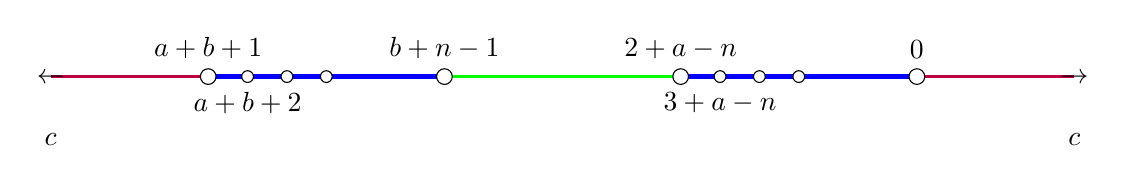
\begin{tikzpicture}
% a straight line segment
\draw[thick,color=purple] (0,0) -- (13,0);
\draw[ultra thick,color=blue] (2,0) -- (5,0);
\draw[ultra thick,color=blue] (8,0) -- (11,0);
\draw[thick,color=green] (5,0) -- (8,0);
\node[fill=white,draw=black,circle,inner sep=2pt,label=above:{$a+b+1$}] at (2,0) {};
   \node[fill=white,draw=black,circle,inner sep=1.5pt,label=below:{$a+b+2$}] at (2.5,0) {};
   \node[fill=white,draw=black,circle,inner sep=1.5pt,label=below:{$$}] at (3,0) {};
   \node[fill=white,draw=black,circle,inner sep=1.5pt,label=below:{$$}] at (3.5,0) {};
\node[fill=white,draw=black,circle,inner sep=2pt,label=above:{$b+n-1$}] at (5,0) {};
\node[fill=white,draw=black,circle,inner sep=2pt,label=above:{$2+a-n$}] at (8,0) {};
   \node[fill=white,draw=black,circle,inner sep=1.5pt,label=below:{$3+a-n$}] at (8.5,0) {};
   \node[fill=white,draw=black,circle,inner sep=1.5pt,label=below:{$$}] at (9,0) {};
   \node[fill=white,draw=black,circle,inner sep=1.5pt,label=below:{$$}] at (9.5,0) {};
\node[fill=white,draw=black,circle,inner sep=2pt,label=above:{$0$}] at (11,0) {};
\node at (0,-0.8) {$c$};
\node at (0,-0.025) {$\leftarrow$};
\node at (13,-0.8) {$c$};
\node at (13,-0.025) {$\rightarrow$};
\end{tikzpicture}

The following remarks are based on observations:
\begin{mydef3}
\item[i)]
When \textcolor{purple}{$c<a+b+1$} or \textcolor{purple}{$0<c$} the generalised Jacobi polynomials $\widehat{\J}_{a,b,c}^{(n)}$ roots take the form of $-a\times n$ ``axe''. The parameters $-a$ and $n$ govern the number of ``columns'' and ``rows'' of the roots, respectively. If $c<a+b+1$ then the ``axe'' will have its longer side directed to the right. However, if $0<c$ then the longer side of the ``axe'' will be directed to the left.
\item[ii)]
When \textcolor{green}{$b+n-1<c<2+a-n$} the generalised Jacobi polynomials $\widehat{\J}_{a,b,c}^{(n)}$ roots take the form of $n\times -a$ ``double axe''. The parameters $n$ and $-a$ govern the number of ``columns'' and ``rows'' of the roots, respectively.
\item[iii)]
When \textcolor{blue}{$c=\{a+b+1,a+b+2,...,b+n-1\}$} or \textcolor{blue}{$c=\{2+a+n,3+a+n,..,0\}$} the generalised Jacobi polynomials $\widehat{\J}_{a,b,c}^{(n)}$ will have at least double roots.
For example: Take $a=-5,~b=-14,~n=5$. The collision points (at least double roots) are $c=\{-18,-17,..,-10\}$ and $c=\{-8,-7,..,0\}$. If $c$ is inside these sets of points we know the roots will form the shapes we saw in figure \ref{P66}.
\item[iv)]
The generalised Jacobi polynomials $\widehat{\J}_{a,b,c}^{(n)}$ have degree equal to $-an$.
\item[v)]
The generalised Jacobi polynomials $\widehat{\J}_{a,b,c}^{(n)}$ always have $-an$ roots.
\end{mydef3}
\normalsize
\subsection{Rational function solutions to the \P equations}
In this section the solutions that are of real interest are the bounded solutions. This is because the applications involving orthogonal always involve the bounded solutions. These bounded solutions are easy to find if we think about the real roots of the polynomials that comprise them. The following theorem explains that a real root, $a$, in our polynomial solutions, regardless of its order, will result in an explosion at $x=a$. Assuming there is no common root between the comprising polynomials, there is no way in which the logarithmic derivative can cancel with the corresponding root.
\begin{mydef}
Given a solution of the form $$w=A(z)+B(z)\frac{d}{dz}\ln \frac{C(z)}{D(z)},$$
where $A(z)$, $B(z)$, $C(z)$ and $D(z)$ are polynomials in $z$. If there exists a real root of $C(z)$ or $D(z)$ we will have an unbounded solution along the real axis, assuming the root is not common between them.
\end{mydef}
\begin{proof}
The first thing to consider is that the solution can be rewritten as
$$w=A(z)+B(z)\frac{d}{dz}\bigg(\ln{C(z)}-\ln D(z)\bigg),$$
Then we assume $(x-a)^n$ divides $C(z)$ or $D(z)$. Does this imply $(z-a)$ divides $\frac{d}{dz}\ln C(z)$?
This implies that $C(z)$ can be written in the form $C(z)=(z-a)^ng(z)$. Differentiating yields $$\frac{dC(z)}{dz}=n(z-a)^{n-1}g(z)+(z-a)^n\frac{dg(z)}{dz}.$$
So,
\begin{align}
\frac{d}{dz}\ln C(z)&=\frac{n(z-a)^{n-1}g(z)+(z-a)^n\frac{dg(z)}{dz}}{(z-a)^ng(z)}\\
&=\frac{n}{z-a}+\frac{d}{dz}\ln g(z).
\end{align}
This implies that the order $n$ of a root is not important and that if a real root exists the root cannot vanish with the logarithmic derivative. If there is a single uncommon real root the solution will not be bounded. Some of the root plots that follow show some unbounded solutions, however, this is purely an illustration that these cases are easily identifiable using the associated root plots.
\end{proof}
\subsubsection{The second \P equation}
\begin{mydef}
The rational solutions to $P_{II}$ \eqref{PII} exist if and only if $A=n\in\Z$, which are unique.
Suppose $Q_n(z)$ is the Yablonskii-Vorob'ev polynomial defined by \eqref{YabDDE}, then the rational solutions of $P_{II}$ \eqref{PII} in the form $w_n(z;A)$ are given by the following:
\begin{equation}
w_n(z;A)=\frac{d}{dz}\bigg\{\ln\bigg[\frac{Q_{n-1}(z)}{Q_n(z)}\bigg]\bigg\},
\end{equation}
for the parameter $A=n$.
\end{mydef}
\begin{proof}
See \cite{P:1:59,P:3:35,P:159:200,P:159:111}.
\end{proof}
The rational solutions to $P_{II}$ \eqref{PII} have no bounded solutions due to the polynomials that generate them always having real roots. This can be seen clearly in the following plots.
\begin{figure}[H]
\centering
\subfigure[$w_3$,]{
\includegraphics[scale=0.26]{P2RFS[n=3]}}
\subfigure[$w_4$,]{
\includegraphics[scale=0.26]{P2RFS[n=4]}}
\subfigure[$w_5$,]{
\includegraphics[scale=0.26]{P2RFS[n=5]}}
\subfigure[$w_6$,]{
\includegraphics[scale=0.26]{P2RFS[n=6]}}
\subfigure[$w_7$,]{
\includegraphics[scale=0.26]{P2RFS[n=7]}}
\subfigure[$w_8$,]{
\includegraphics[scale=0.26]{P2RFS[n=8]}}
\caption{Some rational solutions to $P_{II}$ \eqref{PII} super imposed with the complex roots of the corresponding Yablonskii-Vorob'ev polynomials which comprise the solutions.}
\end{figure}
\subsubsection{The third \P equation}
The locations of the rational solutions of $P_{III}$ \eqref{PIII} solutions are stated the following theorem:
\begin{mydef}
$P_{III}$ \eqref{PIII} with $\gamma=-\delta=1$, has rational solutions if and only if $\alpha+\varepsilon\beta=4n$, with $n\in\Z$ and $\varepsilon=\pm1$. These rational solutions have the form $$w=\frac{P_m(z)}{Q_m(z)},$$
where $P_m(z)$, $Q_m(z)$ are polynomials of degree $m$ with no common roots.
\end{mydef}
\begin{proof}
See Lukashevich \cite{P:3:999}; also Milne, Clarkson and Bassom \cite{P:98:194} and Murata \cite{P:139:65}.
\end{proof}
Suppose $\tau_{a,b}(z)$ is the generalised associated Laguerre polynomial defined by \eqref{P3DDR}, then the rational solutions of $P_{III}$ \eqref{PIII} in the form $$w^{[N]}_n(z;A^{[N]},B^{[N]},C^{[N]},D^{[N]}),$$ for $N=1,..,4$ are given by the following:

\begin{subequations}
\begin{align}
w^{[1]}_n(z;A^{[1]},B^{[1]},C^{[1]},D^{[1]})&=1-\frac{d}{dz}\ln\frac{\tau_{\mu+1,n+1}(z)}{\tau_{\mu,n}(z)},\\
w^{[2]}_n(z;A^{[2]},B^{[2]},C^{[2]},D^{[2]})&=1+\frac{d}{dz}\ln\frac{\tau_{\mu,n+1}(z)}{\tau_{\mu+1,n}(z)},
\end{align}
\end{subequations}
for the parameters
\begin{subequations}
\begin{align}
\{A^{[1]},B^{[1]},C^{[1]},D^{[1]}\}&=\{2(n+\mu)+3,2(n-\mu)+1,1,-1\},\\
\{A^{[2]},B^{[2]},C^{[2]},D^{[2]}\}&=\{-2(n-\mu)-1,-2(n+\mu)-3,1,-1\}.
\end{align}
\end{subequations}
These rational solutions are identical to the Umemura rational solutions. However, the Umemura polynomials are actually polynomials in $1/z$ rather than polynomials in $z$. Clarkson in \cite{P:36:9532} determined special polynomials associated with the rational solutions of $P_{III}$ \eqref{PIII}, which were polynomials in $z$. The rational solutions are shown below in terms of these polynomials.
\begin{mydef}
Suppose $S_n(z;\mu)$ is the Umemura polynomial defined by
$$S_{n+1}S_{n-1}=-z\bigg[S_n\frac{d^2S_n}{dz^2}-\bigg(\frac{dS_n}{dz}\bigg)^2\bigg]-S_n\frac{dS_n}{dz}+(z+\mu)S_n^2$$
with $S_{-1}(z;\mu)=S_0(z;\mu)=1$ \cite{P:36:9532}
(but with the transformation $z\rightarrow1/z$) then the rational solutions of $P_{III}$ \eqref{PIII} are the following:
\begin{subequations}
\begin{align}
w_n=w(z;A^{[1]},B^{[1]},C^{[1]},D^{[1]})&=1+\frac{d}{dz}\bigg\{\ln\bigg[\frac{S_{n-1}(z;\mu-1)}{S_n(z;\mu)}\bigg]\bigg\}\\
&=\frac{S_n(z;\mu-1)S_{n-1}(z;\mu)}{S_n(z;\mu)S_{n-1}(z;\mu-1)},\\
\hat w_n=w(z;A^{[2]},B^{[2]},C^{[2]},D^{[2]})&=1+\frac{d}{dz}\bigg\{\ln\bigg[\frac{S_{n-1}(z;\mu)}{S_n(z;\mu-1)}\bigg]\bigg\}\\
&=\frac{S_n(z;\mu)S_{n-1}(z;\mu-1)}{S_n(z;\mu-1)S_{n-1}(z;\mu)},
\end{align}
\end{subequations}
for the parameters
\begin{subequations}
\begin{align}
\{A^{[1]},B^{[1]},C^{[1]},D^{[1]}\}&=\{2n+2\mu-1,2n-2\mu+1,1,-1\},\\
\{A^{[2]},B^{[2]},C^{[2]},D^{[2]}\}&=\{-2n+2\mu-1,-2n-2\mu+1,1,-1\}.
\end{align}
\end{subequations}
\end{mydef}
\begin{proof}
See \cite{P:36:9532}, which generalizes the work of Kajiwara and Masuda \cite{P:A260:467}.
\end{proof}
The rational solutions of $P_{III}$ have no bounded solutions due to the polynomials that generate them always having real roots. This can be seen clearly in the following plots:
\begin{figure}[H]
\centering
\subfigure[$w^{[1]}_3(z;\mu=-10)$]{
\includegraphics[scale=0.3]{P3RFS[n=3-nu=-10]}}
\subfigure[$w^{[1]}_4(z;\mu=-10)$]{
\includegraphics[scale=0.3]{P3RFS[n=4-nu=-10]}}
\subfigure[$w^{[1]}_5(z;\mu=-10)$]{
\includegraphics[scale=0.3]{P3RFS[n=5-nu=-10]}}
\subfigure[$w^{[1]}_6(z;\mu=-10)$]{
\includegraphics[scale=0.3]{P3RFS[n=6-nu=-10]}}
\caption{Some rational solutions to $P_{III}$ \eqref{PIII} with the complex roots of the corresponding generalised associated Laguerre polynomials which comprise the solutions.}
\end{figure}
\begin{figure}[H]
\centering
\subfigure[$w^{[1]}_3(z;\mu=10)$]{
\includegraphics[scale=0.3]{P3RFS[n=3-nu=10]}}
\subfigure[$w^{[1]}_4(z;\mu=10)$]{
\includegraphics[scale=0.3]{P3RFS[n=4-nu=10]}}
\subfigure[$w^{[1]}_5(z;\mu=10)$]{
\includegraphics[scale=0.3]{P3RFS[n=5-nu=10]}}
\subfigure[$w^{[1]}_6(z;\mu=10)$]{
\includegraphics[scale=0.3]{P3RFS[n=6-nu=10]}}
\caption{Some rational solutions to $P_{III}$ \eqref{PIII} super imposed with the complex roots of the corresponding generalised associated Laguerre polynomials which comprise the solutions.}
\end{figure}
\subsubsection{The fourth \P equation}
\begin{mydef}
$P_{IV}$ has rational solutions if and only if the parameters $A$ and $B$ are given by
\begin{equation}
A=m, \hspace{10mm} B=-2(2n-m+1)^2 \label{p},
\end{equation}
\begin{center}
or
\end{center}
\begin{equation}
A=m, \hspace{10mm} B=-2(2n-m+\tfrac{1}{3})^2, \label{q}
\end{equation}
with m, n $\in$ Z.
\end{mydef}
\begin{proof}
See Lukashevich \cite{P:3:395}, Gromak \cite{P:23:506} and Murata \cite{P:28:32}; also see Bassom, Clarkson and Hicks \cite{P:95:71}, Gromak, Laine and Shimomura \cite{deGruyerCo}, Umemura and Watanabe \cite{P:148:198}.
\end{proof}
\begin{mydef}
Suppose $H_{m,n}(z)$ is the generalised Hermite polynomial defined by \eqref{HermiteRR}, then the rational solutions of $P_{IV}$ \eqref{PIV} in the form $$w^{[N]}_{m,n}=w(z;A^{[N]},B^{[N]}),$$ for $N=1,2,3$ are given by the following:
\begin{subequations}
\begin{align*}\nonumber
w^{[1]}_{m,n}&=w(z;A^{[1]},B^{[1]})=\frac{d}{dz}\ln\Bigg{(}\frac{H_{m+1,n}(z)}{H_{m,n}(z)}\Bigg{)},\\
w^{[2]}_{m,n}&=w(z;A^{[2]},B^{[2]})=\frac{d}{dz}\ln\Bigg{(}\frac{H_{m,n}(z)}{H_{m,n+1}(z)}\Bigg{)},\\
w^{[3]}_{m,n}&=w(z;A^{[3]},B^{[3]})=-2z+\frac{d}{dz}\ln\Bigg{(}\frac{H_{m,n+1}(z)}{H_{m+1,n}(z)}\Bigg{)}.
\end{align*}
\end{subequations}
for the parameters
\begin{subequations}
\begin{align*}\nonumber
\{A^{[1]},B^{[1]}\}&=\{2m+n+1,-2n^2\},\\
\{A^{[2]},B^{[2]}\}&=\{-(m+2n+1),-2m^2\},\\
\{A^{[3]},B^{[3]}\}&=\{n-m,-2(m+n+1)^2\}.
\end{align*}
\end{subequations}
\end{mydef}
\begin{proof}
See Noumi and Yamada \cite{P:153:86}; and also Theorem $3.1$ in Clarkson \cite{P:44:5374}.
\end{proof}
All the rational solutions of $P_{IV}$ \eqref{PIV} with parameters given by \eqref{p} can be expressed in terms of determinants whose entries are Hermite polynomials.

The generalised Hermite polynomials rational solutions of $P_{IV}$ \eqref{PIV} have bounded solutions when $n$ is even. However, they are only bounded from the first hierarchy $w^{[1]}$ due to the formation of the root structures. From the other two hierarchies you cannot get real roots simultaneously from both the polynomials in the rational functions.


\begin{figure}[H]
\centering
\subfigure[$w^{[1]}(z;m=2,n=2)$]{
\includegraphics[scale=0.26]{P4H1[2-2]}}
\subfigure[$w^{[1]}(z;m=4,n=4)$]{
\includegraphics[scale=0.26]{P4H1[4-4]}}
\subfigure[$w^{[1]}(z;m=6,n=6)$]{
\includegraphics[scale=0.26]{P4H1[6-6]}}
\subfigure[$w^{[1]}(z;m=8,n=8)$]{
\includegraphics[scale=0.26]{P4H1[8-8]}}
\subfigure[$w^{[1]}(z;m=10,n=10)$]{
\includegraphics[scale=0.26]{P4H1[10-10]}}
\subfigure[$w^{[1]}(z;m=12,n=12)$]{
\includegraphics[scale=0.26]{P4H1[12-12]}}
\caption{Some rational solutions to $P_{IV}$ \eqref{PIV} super imposed with the complex roots of the corresponding generalised Hermite polynomials which comprise the solutions.}
\end{figure}

Now we consider the generalised Okamoto polynomials.
\begin{mydef}
Suppose $Q_{m,n}(z)$ is the generalised Okamoto polynomial defined by \eqref{OkamotoRR}, then the rational solutions of $P_{IV}$ \eqref{PIV} in the form $$\hat{w}^{[N]}_{m,n}=w(z;A^{[N]},B^{[N]}),$$ are the following:
\begin{subequations}
\begin{align*}
\hat{w}^{[1]}_{m,n}&=w(z;A^{[1]},B^{[1]})=-\frac{2}{3}z+\frac{d}{dz}\bigg(\frac{Q_{m+1,n}(z)}{Q_{m,n}(z)}\bigg),\\
\hat{w}^{[2]}_{m,n}&=w(z;A^{[2]},B^{[2]})=-\frac{2}{3}z+\frac{d}{dz}\bigg(\frac{Q_{m,n}(z)}{Q_{m,n+1}(z)}\bigg),\\
\hat{w}^{[3]}_{m,n}&=w(z;A^{[3]},B^{[3]})=-\frac{2}{3}z+\frac{d}{dz}\bigg(\frac{Q_{m,n+1}(z)}{Q_{m+1,n}(z)}\bigg),
\end{align*}
\end{subequations}
for the parameters
\begin{subequations}
\begin{align*}
\{A^{[1]},B^{[1]}\}&=\{2m+n,-2(n-\tfrac{1}{3})^2\},\\
\{A^{[2]},B^{[2]}\}&=\{-m-2n,=-2(m-\tfrac{1}{3})^2\},\\
\{A^{[3]},B^{[3]}\}&=\{n-m,=-2(m+n+\tfrac{1}{3})^2\}.
\end{align*}
\end{subequations}
\end{mydef}
\begin{proof}
See Noumi and Yamada \cite{P:153:86}; and also Theorem $4.1$ in Clarkson \cite{P:44:5374}.
\end{proof}
The generalised Okamoto rational solutions of $P_{IV}$ \eqref{PIV} have no bounded solutions due to the polynomials that generate them always having real roots. This can be seen clearly in the following plots:

\begin{figure}[H]
\centering
\subfigure[$\hat{w}^{[1]}(z;m=2,n=2)$]{
\includegraphics[scale=0.3]{P4O1[2-2]}}
\subfigure[$\hat{w}^{[1]}(z;m=3,n=3)$]{
\includegraphics[scale=0.3]{P4O1[3-3]}}
\subfigure[$\hat{w}^{[1]}(z;m=4,n=4)$]{
\includegraphics[scale=0.3]{P4O1[4-4]}}
\subfigure[$\hat{w}^{[1]}(z;m=5,n=5)$]{
\includegraphics[scale=0.3]{P4O1[5-5]}}
\caption{Some rational solutions to $P_{IV}$ \eqref{PIV} super imposed with the complex roots of the corresponding generalised Okamoto polynomials which comprise the solutions.}
\end{figure}

\subsubsection{The fifth \P equation}
\begin{mydef}
$P_{V}$ \eqref{PV} has rational solutions if and only if one of the following holds with $m,n\in\Z$ and $\varepsilon=\pm1$:
\begin{itemize}
\item[i)]
$A=\tfrac{1}{2}(m+\varepsilon)^2$ and $B=-\tfrac{1}{2}n^2$, where $n>0$, $m+n$ is odd and $A\ne0$ where $|m|<n$,
\item[ii)]
$A = \tfrac{1}{2}n^2$ and $B = -\tfrac{1}{2}(m+\varepsilon)^2$, where $n > 0$, $m+n$ is odd and $B\ne0$ when $|m|<n$,
\item[iii)]
$A = \tfrac{1}{2}a$ and $B = -\tfrac{1}{2}(a+n)^2$ and $C=m$, where $m+n$ is even and $a$ arbitrary,
\item[iv)]
$A = \tfrac{1}{2}(b+n)$, $B = -\tfrac{1}{2}(b)^2$ and $C=m$, where $m+n$ is even and $b$ arbitrary,
\item[v)]
$A=\tfrac{1}{8}(2m+1)^2$ and $B=-\tfrac{1}{8}(2n+1)^2$.
\end{itemize}
\begin{proof}
See Kitaev, Law and McLeod \cite{P:7:1000}; also Gromak and Lukashevich \cite{P:18:317}; Gromak, Laine and Shimomura \cite{deGruyerCo}.
\end{proof}
\end{mydef}
\begin{mydef}
Suppose $\widetilde{\L}_{\alpha,\beta}^{(n)}(z)$, $\widetilde{\L}_{\alpha,\beta,e^{-z}}^{(n)}(z)$ and ${\L}_{\alpha,\beta}^{(n)}(z)$ are the generalised associated Laguerre polynomials defined by \eqref{L11}, \eqref{L22} and \eqref{L33} then the rational solutions of $P_{V}$ \eqref{PV} in the form $w_n^{[N]}(z;A^{[N]},B^{[N]},C^{[N]},D^{[N]},\varepsilon_3)$ for $N=1,2$ are given by the following:
\begin{subequations}
\begin{align}\nonumber
w_n^{[1]}(z;A^{[1]},B^{[1]},C^{[1]},D^{[1]},1)&=1+\frac{1}{\alpha-\beta-n}\bigg\{\beta+z+z\frac{d}{dz}\ln\frac{\mathcal{\widetilde L}_{\alpha,\beta+1,e^{-z}}^{~(n+1)}(z)}{\mathcal{\widetilde L}_{\alpha,\beta,e^{-z}}^{~(n)}(z)}\bigg\}\\\nonumber
&=1+\frac{1}{\alpha-\beta-n}\bigg\{\beta+z\frac{d}{dz}\ln\frac{\mathcal{\widetilde L}_{\alpha-n,\beta+1}^{~(n+1)}(z)}{\mathcal{\widetilde L}_{\alpha-n+1,\beta}^{~(n)}(z)}\bigg\}\\\nonumber
&=1+\frac{1}{\alpha-\beta-n}\bigg\{\beta+n+z\frac{d}{dz}\ln\frac{\mathcal{ L}_{\alpha-n+1,\beta-n+2}^{~(n+1)}(z)}{\mathcal{ L}_{\alpha-n+1,\beta-n+1}^{~(n)}(z)}\bigg\},\\\nonumber
w_n^{[2]}(z;A^{[2]},B^{[2]},C^{[2]},D^{[2]},-1)&=1+\frac{1}{\alpha+
n}\bigg\{z-\beta-z\frac{d}{dz}\ln\frac{\mathcal{\widetilde L}_{\alpha+1,\beta+1}^{~(n+1)}(z)}{\mathcal{\widetilde L}_{\alpha,\beta}^{~(n)}(z)}\bigg\}\\\nonumber
&=1+\frac{1}{\alpha+n}\bigg\{2z-\beta-z\frac{d}{dz}\ln\frac{\mathcal{\widetilde L}_{\alpha+n+1,\beta+1,e^{-z}}^{~(n+1)}(z)}{\mathcal{\widetilde L}_{\alpha+n-1,\beta,e^{-z}}^{~(n)}(z)}\bigg\}\\\nonumber
&=1+\frac{1}{\alpha+n}\bigg\{z-\beta-n-z\frac{d}{dz}\ln\frac{\mathcal{L}_{\alpha+1,\beta-n+1}^{~(n+1)}(z)}{\mathcal{L}_{\alpha,\beta-n+1}^{~(n)}(z)}\bigg\},
\end{align}
\end{subequations}
for the parameters
\begin{subequations}
\begin{align}
\{A^{[1]},B^{[1]},C^{[1]},D^{[1]}\}&=\{\tfrac{1}{2}(-\alpha+\beta+n)^2,-\tfrac{1}{2}\alpha^2,1+n-\beta,-\tfrac{1}{2}\},\label{J1}\\
\{A^{[2]},B^{[2]},C^{[2]},D^{[2]}\}&=\{\tfrac{1}{2}(\alpha+n)^2,-\tfrac{1}{2}(\beta-\alpha)^2,\beta-n-1,-\tfrac{1}{2}\}.\label{J2}
\end{align}
\end{subequations}
\end{mydef}
\begin{proof}
Taking $\alpha$ to be a negative integer we can apply the polynomial reduction of $U(a,b;z)$ and $M(a,b;z)$ the Kummer functions \eqref{Laguerretrans}, to the special function solutions of $P_{V}$ with a suitable transformation of the parameters yields the rational solutions:
\end{proof}
The rational solutions to $P_{V}$ \eqref{PV} have bounded solutions from the second hierarchy precisely when $1+\alpha-n$ is even for $\beta<0$ with $C_1=0$ or $C_2=0$. This is the exact condition which removes the possibility for real roots.
\begin{figure}[H]
\centering
\subfigure[$w_2^{[2]}(z;\alpha=-5,\beta=-30)$]{
\includegraphics[scale=0.26]{P5RS[-5]30]2]}}
\subfigure[$w_3^{[2]}(z;\alpha=-6,\beta=-30)$]{
\includegraphics[scale=0.26]{P5RS[-6]30]3]}}
\subfigure[$w_4^{[2]}(z;\alpha=-7,\beta=-30)$]{
\includegraphics[scale=0.26]{P5RS[-7]30]4]}}
\subfigure[$w_5^{[2]}(z;\alpha=-8,\beta=-30)$]{
\includegraphics[scale=0.26]{P5RS[-8]30]5]}}
\subfigure[$w_6^{[2]}(z;\alpha=-9,\beta=-30)$]{
\includegraphics[scale=0.26]{P5RS[-9]30]6]}}
\subfigure[$w_7^{[2]}(z;\alpha=-10,\beta=-30)$]{
\includegraphics[scale=0.26]{P5RS[-10]30]7]}}
\caption{Some rational solutions to $P_{V}$ \eqref{PV} super imposed with the complex roots of the corresponding generalised Laguerre polynomials which comprise the solutions.}
\end{figure}
\subsubsection{The sixth \P equation}
\begin{mydef}
$P_{VI}$ \eqref{PVI} has rational solutions if and only if
$$h_1+h_2+h_3+h_4=2n+1,$$
with $\varepsilon_j=\pm1$, $j=1,2,3,4$ independently where $h_1=\varepsilon_1\sqrt{2A}$, $h_2=\varepsilon_2\sqrt{-2B}$, $h_3=\varepsilon_3\sqrt{2C}$, $h_4=\varepsilon_4\sqrt{1-2D}$ and $a\in\Z$.
\end{mydef}
\begin{proof}
See Mazzocco \cite{P:34:2294}. These are special cases of the special function solutions
which we discussed earlier.
\end{proof}

Suppose $\widehat{\J}_{a,b,c}^{(n)}(z)$ is the generalised Jacobi polynomial defined by \eqref{JDDR}, then the rational solutions of $P_{VI}$ \eqref{PVI} in the form $w_n(z;A,B,C,D)$ are given by the following:
\begin{equation}\nonumber
w_n(z;A,B,C,D)=\frac{1}{a}\Bigg\{n+c-(2n+b+1)z-z(z-1)\frac{d}{dz}\ln\frac{{\J}_{a+1,b+1,c+1}^{(n+1)}(z)}{{\J}_{a-1,b+1,c}^{(n)}(z)}\Bigg\},
\end{equation}
for the parameters
$$\{A,B,C,D\}=\{\tfrac{a^2}{2},-\tfrac{1}{2}(b-c+n+1)^2,\tfrac{1}{2}(a-c-n)^2,\tfrac{1}{2}(1-b^2)\},$$
with
$$
{\J}_{a,b,c}^{(n)}=z^{n/2(1-n-2b)}(z-1)^{n(1-n)/2}\widehat{\J}_{a,b,c}^{(n)}.
$$
\begin{figure}[H]
\centering
\subfigure[$w_4(z;a\!=\!-7,b\!=\!-16,c\!=\!-11)-L(z)$]{
\includegraphics[scale=0.35]{P6RS4[-7-16-11]}}
\subfigure[$w_5(z;a\!=\!-9,b\!=\!-18,c\!=\!-13)-L(z)$]{
\includegraphics[scale=0.35]{P6RS5[-9-18-13]}}
\subfigure[$w_6(z;a\!=\!-11,b\!=\!-20,c\!=\!-15)-L(z)$]{
\includegraphics[scale=0.35]{P6RS6[-11-20-15]}}
\subfigure[$w_7(z;a\!=\!-13,b\!=\!-22,c\!=\!-17)-L(z)$]{
\includegraphics[scale=0.35]{P6RS7[-13-22-17]}}
\caption{Some rational solutions to $P_{VI}$ \eqref{PVI} super imposed with the complex roots of the corresponding generalised Jacobi polynomials which comprise the solutions, where $L(z)$ is the asymptotic behaviour around $\pm \infty$.}
\end{figure}
The rational solutions to $P_{VI}$ have bounded solutions precisely when $b+n-1<c<2+a-n$ and $-a$ is even. This is exactly the condition that removes the possibility for real roots.
\subsection{Rational function solutions to the $\sigma$-equations}
\subsubsection{The second \P $\sigma$-equation}
\begin{mydef}
Suppose $Q_n(z)$ is the Yablonskii-Vorob'ev polynomial defined by \eqref{YabDDE}, then the rational solutions of $S_{II}$ \eqref{SII} in the form $\sigma_n(z;\alpha)$ are given by the following:
\begin{equation}
\sigma_n(z;\alpha)=-\frac{1}{8}z^2+\frac{d}{dz}\ln Q_n(z),
\end{equation}
for the parameter $\alpha=n$.
\end{mydef}
\begin{proof}
See \cite{deGruyerCo}.
\end{proof}
The rational solutions to $S_{II}$ \eqref{SII} have no bounded solutions due to the polynomials that generate them always having real roots.
\begin{figure}[H]
\centering
\subfigure[$\sigma_3$,]{
\includegraphics[scale=0.26]{S2RFS[n=3]}}
\subfigure[$\sigma_4$,]{
\includegraphics[scale=0.26]{S2RFS[n=4]}}
\subfigure[$\sigma_5$,]{
\includegraphics[scale=0.26]{S2RFS[n=5]}}
\subfigure[$\sigma_6$,]{
\includegraphics[scale=0.26]{S2RFS[n=6]}}
\subfigure[$\sigma_7$,]{
\includegraphics[scale=0.26]{S2RFS[n=7]}}
\subfigure[$\sigma_8$,]{
\includegraphics[scale=0.26]{S2RFS[n=8]}}
\caption{Some rational solutions to $S_{II}$ \eqref{SII} super imposed with the complex roots of the corresponding Yablonskii-Vorob'ev polynomials which comprise the solutions.}
\end{figure}
\subsubsection{The third \P $\sigma$-equation}
\begin{mydef}
Suppose $\tau_{a,b}(z)$ is the generalised associated Laguerre polynomial defined by \eqref{P3DDR}, then the rational solutions of $S_{III}$ \eqref{SIII} in the form $\sigma_{\mu,n}(z;\vartheta_0,\vartheta_\infty)$ are given by the following:
\begin{equation}
\sigma_{\mu,n}(z;\vartheta_0,\vartheta_\infty)=-\frac{1}{4}z^2-\mu z+\frac{1}{8}+z\frac{d}{dz}\ln\tau_{\mu,n}(z),
\end{equation}
for the parameters $$\{\vartheta_0,\vartheta_\infty\}=\{\mu^2+(n+\tfrac{1}{2})^2,\mu^2-(n+\tfrac{1}{2})^2\}.$$
\end{mydef}
\begin{proof}
These results can be inferred from the work of Clarkson in \cite{P:36:9532}.
\end{proof}
The rational solutions to $S_{III}$ \eqref{SIII} have no bounded solutions due to the polynomials that generate them always having real roots and their symmetric triangular structure.

\begin{figure}[H]
\centering
\subfigure[$\sigma_{3,10}(z)$]{
\includegraphics[scale=0.26]{S3RFS[3-10]}}
\subfigure[$\sigma_{3,-10}(z)$]{
\includegraphics[scale=0.26]{S3RFS[3--10]}}
\subfigure[$\sigma_{4,10}(z)$]{
\includegraphics[scale=0.26]{S3RFS[4-10]}}
\subfigure[$\sigma_{4,-10}(z)$]{
\includegraphics[scale=0.26]{S3RFS[4--10]}}
\subfigure[$\sigma_{5,10}(z)$]{
\includegraphics[scale=0.26]{S3RFS[5-10]}}
\subfigure[$\sigma_{5,-10}(z)$]{
\includegraphics[scale=0.26]{S3RFS[5--10]}}
\caption{Some rational solutions to $S_{III}$ \eqref{SIII} super imposed with the complex roots of the corresponding generalised associated Laguerre which comprise the solutions.}
\end{figure}

\subsubsection{The fourth \P $\sigma$-equation}
\begin{mydef}
Suppose $H_{m,n}(z)$ is the generalised Hermite polynomial defined by \eqref{HermiteRR}, then the rational solutions of $S_{IV}$ \eqref{SIV} in the form $\sigma^{[N]}_{m,n}(z;\vartheta_0^{[N]},\vartheta_\infty^{[N]})$ for $N=1,2,3$ are given by the following:
\begin{subequations}
\begin{align}
\sigma^{[1]}_{m,n}(z;\vartheta_0^{[1]},\vartheta_\infty^{[1]})&=\frac{d}{dz}\ln H_{m,n}(z),\\
\sigma^{[2]}_{m,n}(z;\vartheta_0^{[2]},\vartheta_\infty^{[2]})&=\frac{d}{dz}\ln H_{m,n}(z)-2nz,\\
\sigma^{[3]}_{m,n}(z;\vartheta_0^{[3]},\vartheta_\infty^{[3]})&=\frac{d}{dz}\ln H_{m,n}(z)+2mz,
\end{align}
\end{subequations}
for the parameters
\begin{subequations}
\begin{align}
\{\vartheta_0^{[1]},\vartheta_\infty^{[1]}\}&=\{-n,m\},\\
\{\vartheta_0^{[2]},\vartheta_\infty^{[2]}\}&=\{n,m+n\},\\
\{\vartheta_0^{[3]},\vartheta_\infty^{[3]}\}&=\{-m,-m-n\}.\label{S3TH}
\end{align}
\end{subequations}
\end{mydef}
\begin{proof}
Taking $\nu$ to be an integer, $m$, we can apply the polynomial reduction of $D_\nu(z)$ the parabolic cylinder function \eqref{PCF1}, \eqref{PCF2} and \eqref{PCF3} to the special function solutions of $S_{IV}$ with a suitable transformation of the parameters yields the rational solutions: Also see Okamoto \cite{P:275:221}; also Forrester and Witte \cite{P:219:357}.
\end{proof}
The rational solutions to $S_{IV}$ have bounded solutions precisely when $n$ is even. However, only \eqref{S3TH} omits bounded solutions due to the linear component cancelling out the asymptotic behaviour around $\pm\infty$.
\begin{figure}[H]
\centering
\subfigure[$\sigma^{[1]}(z;m=2)$]{
\includegraphics[scale=0.255]{S4SFm2}}
\subfigure[$\sigma^{[1]}(z;m=4)$]{
\includegraphics[scale=0.255]{S4SFm4}}
\subfigure[$\sigma^{[1]}(z;m=6)$]{
\includegraphics[scale=0.255]{S4SFm6}}
\subfigure[$\sigma^{[1]}(z;m=8)$]{
\includegraphics[scale=0.255]{S4SFm8}}
\subfigure[$\sigma^{[1]}(z;m=10)$]{
\includegraphics[scale=0.255]{S4SFm10}}
\subfigure[$\sigma^{[1]}(z;m=12)$]{
\includegraphics[scale=0.255]{S4SFm12}}
\caption{Some rational solutions to $S_{IV}$ \eqref{SIV} super imposed with the complex roots of the corresponding generalised Hermite polynomials which comprise the solutions, with $n=\{$\textcolor{black}{2}, \textcolor{blue}{4}, \textcolor{magenta}{6}, \textcolor{Plum}{8}\}.}
\end{figure}
It is interesting to note that the number of "kinks" in these solutions is equal to $m-1$.
\begin{figure}[H]
\centering
\subfigure[$\sigma^{[1]}(z;m=2,n=2)$]{
\includegraphics[scale=0.34]{P4RSH[2-2]}}
\subfigure[$\sigma^{[1]}(z;m=4,n=4)$]{
\includegraphics[scale=0.34]{P4RSH[4-4]}}
\subfigure[$\sigma^{[1]}(z;m=6,n=6)$]{
\includegraphics[scale=0.34]{P4RSH[6-6]}}
\subfigure[$\sigma^{[1]}(z;m=8,n=8)$]{
\includegraphics[scale=0.34]{P4RSH[8-8]}}
\caption{Some rational solutions to $S_{IV}$ \eqref{SIV} super imposed with the complex roots of the corresponding generalised Hermite polynomials which comprise the solutions.}
\end{figure}
\begin{mydef}
Suppose $Q_{m,n}(z)$ is the generalised Okamoto polynomial defined by \eqref{OkamotoRR}, then the rational solutions of $S_{IV}$ \eqref{SIV} in the form $\sigma^{[1]}_{m,n}(z;\vartheta_0^{[1]},\vartheta_\infty^{[1]})$ for $N=1,2,3$ are given by the following:
\begin{subequations}
\begin{align}
\sigma^{[1]}_{m,n}(z;\vartheta_0^{[1]},\vartheta_\infty^{[1]})&=\tfrac{4}{27}z^3+\tfrac{2}{3}(n-m)z+\frac{d}{dz}\ln Q_{m,n}(z),\\
\sigma^{[2]}_{m,n}(z;\vartheta_0^{[2]},\vartheta_\infty^{[2]})&=\tfrac{4}{27}z^3-\tfrac{2}{3}(m+2n-1)z+\frac{d}{dz}\ln Q_{m,n}(z),\\
\sigma^{[3]}_{m,n}(z;\vartheta_0^{[3]},\vartheta_\infty^{[3]})&=\tfrac{4}{27}z^3+\tfrac{2}{3}(2m+n-1)z+\frac{d}{dz}\ln Q_{m,n}(z),
\end{align}
\end{subequations}
for the parameters
\begin{subequations}
\begin{align}
\{\vartheta_0^{[1]},\vartheta_\infty^{[1]}\}&=\{m-\tfrac{1}{3},\tfrac{1}{3}-n\},\\
\{\vartheta_0^{[2]},\vartheta_\infty^{[2]}\}&=\{n-\tfrac{1}{3},m+n-\tfrac{2}{3}\},\\
\{\vartheta_0^{[3]},\vartheta_\infty^{[3]}\}&=\{\tfrac{2}{3}-m-n,\tfrac{1}{3}-m\}.
\end{align}
\end{subequations}
\end{mydef}
\begin{proof}
These solutions can be inferred from the $P_{IV}$ \eqref{PIV} Okamoto rational function solutions using the Hamiltonian structure of $P_{IV}$ \eqref{PIV}.
\end{proof}

\subsubsection{The fifth \P $\sigma$-equation}
\begin{mydef}
Suppose $\widetilde{\L}_{\alpha,\beta}^{(n)}(z)$, $\widetilde{\L}_{\alpha,\beta,e^{-z}}^{(n)}(z)$ and ${\L}_{\alpha,\beta}^{(n)}(z)$ are the generalised associated Laguerre polynomials defined by \eqref{L11}, \eqref{L22} and \eqref{L33}, then the rational solutions of $S_{V}$ \eqref{SV} in the form $\sigma_n(z;\kappa_0^{[N]},\kappa_1^{[N]},\kappa_2^{[N]},\kappa_3^{[N]},\varepsilon_3)$ for $N=1,2$ are given by the following:
\begin{subequations}
\begin{align}\nonumber
\sigma_n^{[1]}(z;\kappa_0,\kappa_1^{[1]},\kappa_2^{[1]},\kappa_3^{[1]},1)=&z\frac{d}{dz}\ln\mathcal{\widetilde L}_{\alpha,\beta,e^{-z}}^{(n+1)}(z)-\tfrac{5}{8}\,{(n+1)}^{2}+
\tfrac{1}{4}\left(2\alpha+1+\beta+3z\right)\\\nonumber&\qquad
(n+1)-\tfrac{1}{8}\left( -2\,\alpha-1+\beta \right)  \left( -2\,\alpha-1-2\,z+\beta\right)\\\nonumber
=&z\frac{d}{dz}\ln\mathcal{L}_{\alpha-n,\beta-n}^{(n+1)}(z)-\tfrac{1}{8}\,{(n+1)}^{2}+ \tfrac{1}{4}\left(2\alpha-1+\beta-z\right)\\\nonumber&\qquad
(n+1)-\tfrac{1}{8}\left( -2\,\alpha-1+\beta \right)  \left( -2\,\alpha-1-2\,z+\beta\right),\\\nonumber
\sigma_n^{[2]}(z;\kappa_0,\kappa_1^{[2]},\kappa_2^{[2]},\kappa_3^{[2]},-1)
=&z\frac{d}{dz}\ln\mathcal{\widetilde L}_{\alpha+1,\beta+1}^{(n)}(z)-\tfrac{5}{8}\,{n}^{2}+\tfrac{1}{4}\left(3\beta+2-2\,\alpha-3z\right) n\\\nonumber&\qquad
-\tfrac{1}{8}\left( 2\,\alpha-\beta \right)  \left( 2\,\alpha+2\,z-\beta\right)\\\nonumber
=&z\frac{d}{dz}\ln\mathcal{L}_{\alpha+1,\beta-n+2}^{(n)}(z)-\tfrac{1}{8}\,{n}^{2}+\tfrac{1}{4}\left(3\beta-2\,\alpha-3z \right)n\\\nonumber&\qquad
-\tfrac{1}{8}\left( 2\alpha-\beta \right)  \left( 2\alpha+2\,z-\beta\right),
\end{align}
\end{subequations}
for the parameters
\begin{subequations}
\begin{align}\nonumber
\{\kappa_0^{[1]},\kappa_1^{[1]},\kappa_2^{[1]},\kappa_3^{[1]}\}&=\tfrac{1}{4}\{2\alpha-\beta+n+2,n+2-2\alpha-\beta,2\alpha-\beta-3n-2,3\beta+n\\\qquad&-2\alpha-2)\},\\
\{\kappa_0^{[2]},\kappa_1^{[2]},\kappa_2^{[2]},\kappa_3^{[2]}\}&=-\tfrac{1}{4}\{2\alpha+\beta+n,\beta-3n-2\alpha,n+2\alpha-3\beta,\beta+n-2\alpha\}.
\end{align}
\end{subequations}
\end{mydef}
\begin{proof}
Taking $\alpha$ to be a negative integer we can apply the polynomial reduction of $U(a,b;z)$ and $M(a,b;z)$ the Kummer functions \eqref{Laguerretrans}, to the special function solutions of $S_{V}$ with a suitable transformation of the parameters yields the rational solutions:
\end{proof}
The rational solutions of $S_{V}$ have no bounded solutions due
to the asymptotic behaviour around $\pm\infty$ being linear. However, if an appropriate linear transformation is made we can have bounded solutions and this is precisely when the polynomials have no real roots. The conditions for this are specified in the generalised associated Laguerre polynomials chapter with $C_1=0$ or $C_2=0$.

\begin{figure}[H]
\centering
\subfigure[$\sigma_4^{[1]}(z;\alpha\!=\!-8,\beta\!=\!20)-A-\tfrac{n}{2}(3n-1)$]{
\includegraphics[scale=0.33]{S5RFS[4--8-20]}}
\subfigure[$\sigma_4^{[1]}(z;\alpha\!=\!-8,\beta\!=\!-30)-A-\tfrac{n}{2}(3n-1)$]{
\includegraphics[scale=0.33]{S5RFS[4--8--30]}}
\subfigure[$\sigma_6^{[1]}(z;\alpha\!=\!-12,\beta\!=\!20)-A-\tfrac{n}{2}(3n-1)$]{
\includegraphics[scale=0.33]{S5RFS[6--12-20]}}
\subfigure[$\sigma_6^{[1]}(z;\alpha\!=\!-12,\beta\!=\!-30)-A-\tfrac{n}{2}(3n-1)$]{
\includegraphics[scale=0.33]{S5RFS[6--12--30]}}
\caption{Some rational solutions to $S_{V}$ \eqref{SV} super imposed with the complex roots of the corresponding generalised associated Laguerre polynomials which comprise the solutions, where}
\end{figure}
\begin{align*}
A&=-\tfrac{5}{8}\,{(n+1)}^{2}+
\tfrac{1}{4}\left(2\alpha+1+\beta+3z\right) (n+1)\\
&\qquad-\tfrac{1}{8}\left( -2\,\alpha-1+\beta \right)  \left( -2\,\alpha-1-2\,z+\beta\right).
\end{align*}

\subsubsection{The sixth \P $\sigma$-equation}
\begin{mydef}
Suppose $\J_{a,b,c}^{(n)}(z)$ is the generalised Jacobi polynomial defined by \eqref{JDDR}, then the rational solutions of $S_{VI}$ \eqref{SVI} in the form $\sigma(z;\kappa_1,\kappa_2,\kappa_3,\kappa_4)$ are given by the following:
\begin{align*}
\sigma(z;\kappa_1,\kappa_2,\kappa_3,\kappa_4)&=\tfrac{1}{4}\,(n+1) \left( 4\,az-a+b-2\,c+1 \right) -\tfrac{1}{4}\, \left(a-b+1\right) ^{2
}z\\
&\qquad+\tfrac{1}{4} \left(a^2+a+b^2-b-ac-bc\right)+z(z-1)\frac{d}{dz}\ln\J_{a,b,c}^{(n+1)}(z),
\end{align*}
for the parameters
$$
\{\kappa_1,\kappa_2,\kappa_3,\kappa_4\}=\{-\tfrac{1}{2}(a-b-2n-1),\tfrac{1}{2}(a+b-2c+1),-\tfrac{1}{2}(a-b+1),\tfrac{1}{2}(a+b-1)\}.
$$
\end{mydef}
\begin{proof}
Taking $a$ to be a negative integer we can apply the polynomial reduction of the general hypergeometric function $F(a,b,c;z)$ via an appropriate choice of the parameters. Applying this to the special function solutions of $S_{VI}$ \eqref{SVI} gives the desired result.
\end{proof}
The rational solutions of $S_{VI}$ have no bounded solutions due
to the asymptotic behaviour around $\pm\infty$ being linear. However, if an appropriate linear transformation is made we can have bounded solutions and this is precisely when the polynomials have no real roots. The conditions for this are specified in the generalised Jacobi polynomials chapter.

\begin{figure}[H]
\centering
\subfigure[$\widetilde{\sigma_2}({a\!=\!-2,b\!=\!-15,c\!=\!-8})$]{
\includegraphics[scale=0.250]{S6RFS-2[-2-15-8]}}
\subfigure[$\widetilde{\sigma_4}({a\!=\!-4,b\!=\!-13,c\!=\!-8})$]{
\includegraphics[scale=0.250]{S6RFS-4[-4-13-8]}}
\subfigure[$\widetilde{\sigma_3}({a\!=\!-3,b\!=\!-14,c\!=\!30})$]{
\includegraphics[scale=0.250]{S6RFS-3[-3-14--30]}}
\subfigure[$\widetilde{\sigma_3}({a\!=\!-3,b\!=\!-14,c\!=\!-50})$]{
\includegraphics[scale=0.250]{S6RFS-3[-3-14-50]}}
\subfigure[$\widetilde{\sigma_5}({a\!=\!-5,b\!=\!-12,c\!=\!30})$]{
\includegraphics[scale=0.250]{S6RFS-5[-5-12--30]}}
\subfigure[$\widetilde{\sigma_5}({a\!=\!-5,b\!=\!-12,c\!=\!-50})$]{
\includegraphics[scale=0.250]{S6RFS-5[-5-12-50]}}
\caption{Some rational solutions to $S_{VI}$ \eqref{SVI} super imposed with the complex roots of the corresponding generalised Jacobi polynomials which comprise the solutions, with $\widetilde{\sigma_n}(z)=\sigma_n(z)-A(z)$, where $A(z)$ is the asymptotic expansion of the solution around $\pm\infty$.}
\end{figure}


\newpage\section{Monic orthogonal polynomials}
In the following chapter we will be introducing the concept of monic orthogonal polynomials. We will also be discussing classical and semi-classical orthogonal polynomials and their differences.
\subsection{Continuous orthogonal polynomials}
Monic orthogonal polynomials are a certain type of polynomial $p_n(x)$, defined over a range $[a,b]$, that satisfy an orthogonality relation
$$\int^b_aw(x)p_m(x)p_n(x)\,dx=h_n\delta_{mn},\qquad h_n>0,$$
with $n\in\N$, $\delta_{mn}$ the Kroneker delta and $p_n(x)$ an orthogonal polynomial of degree $n$ with respect to a positive weight
$w(x)$.
An important property of orthogonal polynomials is that they must satisfy a three term recurrence relation of the following form:
\begin{equation}
xp_n(x)=p_{n+1}(x)+\alpha_{n}p_n(x)+\beta_np_{n-1}(x),\nonumber
\end{equation}
where the coefficients $\alpha_n$ and $\beta_n$ are given by
\begin{equation}\nonumber
\alpha_n=\frac{1}{h_n}\int^b_axp_n^2(x)w(x)\,dx,\qquad \beta_n=\frac{1}{h_{n-1}}\int^b_axp_{n-1}(x)p_nw(x)\,dx,
\end{equation}
with $p_{-1}=0$ and $p_{0}=1$. One of our aims in this thesis is to find an alternative method for calculating these coefficients using determinants of moments
that are
produced from our associated orthogonal polynomial weight.
The coefficients $\alpha_n$ and $\beta_n$ can be rewritten in the following way:
\begin{equation}
\alpha_n=\frac{\widetilde\Delta_{n+1}}{\Delta_{n+1}}-\frac{\widetilde\Delta_{n}}{\Delta_{n}},\qquad
\beta_n=\frac{\Delta_{n+1}\Delta_{n-1}}{\Delta_n^2}, \label{deltas}
\end{equation}
where $\Delta_n$ and $\widetilde\Delta_n$ are the determinants given by
\begin{equation}\Delta_n:=\begin{vmatrix}
\mu_{0} & \mu_1  &\hdots& \mu_{n-1} \\
\mu_1 & \mu_2  &\hdots& \mu_n  \\
\vdots  &\vdots & \ddots &\vdots & \\
\mu_{n-1} & \mu_n  &\hdots& \mu_{2n-2}
\end{vmatrix},~~n\geq1,
 \label{delta}
 \end{equation}

\begin{equation}\widetilde\Delta_n:=
 \begin{vmatrix}
\mu_{0} & \mu_1  &\hdots& \mu_{n-2} & \mu_{n} \\
\mu_1 & \mu_2  &\hdots& \mu_{n-1} & \mu_{n+1}  \\
\vdots &\vdots  & \ddots & \vdots &\vdots \\
\mu_{n-1} & \mu_n  &\hdots& \mu_{2n-3} & \mu_{2n-1}
 \end{vmatrix},~~n\geq1,
 \label{deltawidetilde}
\end{equation}
and the initial states are $\Delta_0=1$ and $\Delta_{-1}=\widetilde\Delta_0=1$.
The individual moments can be calculated as follows:
\begin{equation}
\mu_k=\int^b_ax^kw(x)\,dx.\label{muk}
\end{equation}
We remark that the Hankel determinant $\Delta_n(z)$ \eqref{delta} also has the integral representation
\begin{equation}
\Delta_n(x)=\frac{1}{n!}\int^b_a\dots\int^b_a\prod^n_{l=1}w(x_l)\!\!\!\!\!\prod_{1\leq j<k\leq n}\!\!\!\!\!(x_j-x_k)^2dx_1,...,dx_n,~~n\geq1.
\end{equation}
This arises in Random matrix theory as the partition function for the unitary ensemble with eigenvalue
distribution. See Mehta \cite{Mehta} for full details.

It is a well known fact that the monic polynomial $p_n(x)$ can be uniquely expressed as the following:
\begin{equation}p_n(x)=\frac{1}{\Delta_n}
 \begin{vmatrix}
\mu_{0} & \mu_1  &\hdots& \mu_{n-1} \\
\mu_1 & \mu_2  &\hdots& \mu_{n}   \\
\vdots &\vdots  & \ddots & \vdots \\
\mu_{n-1} & \mu_n  &\hdots& \mu_{2n-1}  \\
1 & x  &\hdots & x^n
 \end{vmatrix},~~n\geq1
\end{equation}
and the normalisation constant is
$$h_n=\frac{\Delta_{n+1}}{\Delta_n},~~~h_0=\Delta_1=\mu_0.$$
Now suppose the weight has the following form:
\begin{equation}
w(x;z)=w_0(x)\exp(xz),\label{wxexp}
\end{equation}
where $z$ is a parameter with finite moments for all $z\in\R$. If the weight has the form \eqref{wxexp} then suddenly the polynomials $p_n(x)$, the recurrence coefficients $\alpha_n$ and $\beta_n$, the determinants $\Delta_n$, $\widetilde\Delta_n$ and the moments $\mu_k$ are all now functions of $z$. For certain weights, a consequence of \eqref{wxexp} is the following:
\begin{equation}
\mu_k=\pm\frac{d}{dz}\mu_{k\pm1}\label{momentform}
\end{equation}
and the recurrence relation has the form
\begin{equation}
xp_n(x;z)=p_{n+1}(x;z)+\alpha_n(z)p_n(x;z)+\beta_n(z)p_{n-1}(x;z).\label{rr}
\end{equation}
The implementation of \eqref{momentform} in the determinants $\Delta_n$ and $\widetilde\Delta_n$ given by \eqref{delta} has the following effect:
\[\Delta_n=
\begin{vmatrix}
\mu_{0} & \mu'_0  &\hdots& \mu_0^{(n-1)} \\
\mu_0' & \mu''_0  &\hdots& \mu_0^{(n)}  \\
\vdots &\vdots  & \ddots &\vdots & \\
\mu_0^{(n-1)} & \mu_0^{(n)} &\hdots& \mu_0^{(2n-2)}
\end{vmatrix},~~'=\frac{d}{dz},
\]
\[
\widetilde\Delta_n=\left|
\begin{array}{ccccc}
\mu_{0} & \mu_{0}'  &\hdots& \mu_{0}^{(n-2)} & \mu_{j}^{(n)} \\
\mu_{0}' & \mu_{0}''  &\hdots& \mu_{0}^{(n-1)} & \mu_{0}^{(n+1)}  \\
\vdots &\vdots  & \ddots &\vdots &\vdots \\
\mu_{0}^{(n-1)} & \mu_{0}^{(n)}  &\hdots& \mu_{0}^{(2n-3)} & \mu_{0}^{(2n-1)}
\end{array}
\right|,~~'=\frac{d}{dz}.\]
Hence we can construct the following theorem:
\begin{mydef}\label{mo:2}
As before, we will denote $\tau_n$ as the bi-directional \w
\begin{equation}
\tau_n(f)=\W\bigg(f,\frac{df}{dz},...,\frac{d^{n-2}f}{dz^{n-2}},\frac{d^{n-1}f}{dz^{n-1}}\bigg).\label{Wronskian}
\end{equation}
If the moment $\mu_k(z)$ has the form \eqref{momentform} then the determinants $\Delta_n$ and $\widetilde\Delta_n$ can be
written in the form
\begin{equation}\label{dd}
\Delta_n(z)=\tau_n(\mu_0),\qquad\widetilde\Delta_n(z)=\frac{d}{dz}\tau_n(\mu_0).
\end{equation}
\end{mydef}
\begin{proof}
See \cite{Rec,P:44:291,P:30:305,P:62:1887}.
\end{proof}
Also, since $\mu_k=\frac{d^k\mu_j}{dz^k}$, the determinants $\Delta_n(z)$ and $\widetilde\Delta_n(z)$ can be written in the form
\begin{align*}
\Delta_n=\begin{vmatrix}
\mu_{0} & \mu_1  &\hdots& \mu_{n-1} \\
\mu_1 & \mu_2  &\hdots& \mu_n  \\
\vdots  &\vdots & \ddots &\vdots & \\
\mu_{n-1} & \mu_n  &\hdots& \mu_{2n-2}
\end{vmatrix}&=\mathcal{W}\bigg(\mu_0,\frac{d}{dz}\mu_0,...,\frac{d^{n-1}\mu_0}{dz^{n-1}}\bigg)\\
&=\tau_n(\mu_0),\\
\widetilde\Delta_n=\begin{vmatrix}
\mu_{0} & \mu_1  &\hdots& \mu_{n-2} & \mu_{n} \\
\mu_1 & \mu_2  &\hdots& \mu_{n-1} & \mu_{n+1}  \\
\vdots &\vdots  & \ddots & \vdots &\vdots \\
\mu_{n-1} & \mu_n  &\hdots& \mu_{2n-3} & \mu_{2n-1}
\end{vmatrix}&=\mathcal{W}\bigg(\mu_0,\frac{d}{dz}\mu_0,...,\frac{d^{n-2}\mu_0}{dz^{n-1}},\frac{d^{n}\mu_0}{dz^{n}}\bigg)\\
&=\frac{d}{dz}\mathcal{W}\bigg(\mu_0,\frac{d}{dz}\mu_0,...,\frac{d^{n-2}\mu_0}{dz^{n-1}},\frac{d^{n-1}\mu_0}{dz^{n-1}}\bigg)\\
&=\frac{d}{dz}\tau_n(\mu_0).
 \label{delta}
\end{align*}

\begin{mydef}
The Hankel determinant $\Delta_n(z)$ given by \eqref{delta} satisfies the Toda equation
\begin{equation}\label{toda}
\frac{d^2}{dz^2}\ln\Delta_n(z)=\frac{\Delta_{n+1}(z)\Delta_{n-1}(z)}{\Delta_n^2(z)}.
\end{equation}
\end{mydef}
\begin{proof}
See \cite{P:30:54,P:151:528,P:62:1887}.
\end{proof}
\begin{mydef}
As long as the condition \eqref{momentform} is satisfied the recurrence coefficients $\alpha_n(z)$ and $\beta_n(z)$ in \eqref{rr} can be expressed in the form
\begin{equation}
\alpha_n(z)=\frac{d}{dz}\ln\bigg(\frac{\tau_{n+1}(\mu_0)}{\tau_{n}(\mu_0)}\bigg),\qquad \beta_n(z)=\frac{d^2}{dz^2}\!\ln\{\tau_{n}(\mu_0)\}.\label{deltas2}
\end{equation}
\end{mydef}
\begin{proof}
The proof is actually straightforward; applying the theorem \ref{mo:2} to \eqref{deltas} and using that $\Delta_n$ satisfies the Toda equation \eqref{toda} gives the desired result. This is shown in detail below.

Recall that $\alpha_n(z)$ and $\beta_n(z)$ are defined by
\begin{equation}\nonumber
\alpha_n=\frac{\widetilde\Delta_{n+1}}{\Delta_{n+1}}-\frac{\widetilde\Delta_{n}}{\Delta_{n}},\qquad
\beta_n=\frac{\Delta_{n+1}\Delta_{n-1}}{\Delta_n^2},
\end{equation}
where $\Delta_n(z)$ and $\widetilde\Delta_n(z)$ are defined by \eqref{delta} and \eqref{deltawidetilde}. Using \eqref{dd} and \eqref{toda} we can deduce the following:
\begin{align*}
\alpha_n(z)=\frac{\widetilde\Delta_{n+1}(z)}{\Delta_{n+1}(z)}-\frac{\widetilde\Delta_n(z)}{\Delta_n(z)}
&=\frac{1}{\Delta_{n+1}(z)}\frac{d\Delta_{n+1}(z)}{dz}-\frac{1}{\Delta_{n}(z)}\frac{d\Delta_{n}(z)}{dz}\\
&=\frac{d}{dz}\ln \Delta_{n+1}(z)-\frac{d}{dz}\ln \Delta_{n}(z)\\
&=\frac{d}{dz}\bigg\{\ln\Delta_{n+1}(z)-\ln\Delta_{n}(z)\bigg\}\\
&=\frac{d}{dz}\ln\frac{\Delta_{n+1}(z)}{\Delta_{n}(z)},\\
\nonumber\\
\beta_n(z)=\frac{\Delta_{n+1}\Delta_{n-1}}{\Delta_n^2}
&=\frac{d^2}{dz^2}\ln\Delta_n(z),
\end{align*}
as required.
\end{proof}
Some motivation for this work is that the recurrence coefficients of semi-classical orthogonal polynomials can often be expressed in terms of solutions of the \P equations. For example; all the recurrence coefficients can be expressed in terms of solutions of $P_{II}$ \eqref{PII} for semi-classical orthogonal polynomials with respect to an Airy weight
\begin{equation}\label{P2weight}
w(x;z)=\exp(\tfrac{1}{3}x^3+zx),~~~x^3<0,
\end{equation}
with $z\in\R$ a parameter \cite{P:57:37}.
In terms of solutions of $P_{III}$ \eqref{PIII} for the deformed Laguerre weight
\begin{equation}\nonumber
w(x;z)=x^\alpha\exp(-x-z/x),~~~x\in\R^{+},
\end{equation}
with $\alpha>0$ and $z\in\R^{+}$ parameters \cite{P:162:97}.
In terms of solutions of $P_{V}$ \eqref{PV} for the weights
\begin{align}\nonumber
w(x;z)&=(1-x)^\alpha(1+x)^\beta e^{-zx},~~~x\in[-1,1],\\\nonumber
w(x;z)&=x^\alpha(1-x)^\beta e^{-z/x},~~~x\in[0,1],\\\nonumber
w(x;z)&=x^\alpha(x+z)^\beta e^{-x},~~~x\in\R^{+},
\end{align}
with $\alpha, \beta$ $>0$ and $t\in\R^{+}$ parameters \cite{Basor,P:1303.0773,Chen,P:58:4634,P:61:526}.
In terms of solutions of $P_{VI}$ \eqref{PVI} for the weight
\begin{align}\nonumber
w(x;z)&=x^\alpha(1-x)^\beta(z-x)^\gamma,~~~x\in[0,1],
\end{align}
with $\alpha,\beta,\gamma>0$ and $z\in\R^+$ parameters \cite{P:860:463,P:58:4634,P:43:055207,P:57:37}.
\subsubsection{Example - Hermite polynomials}
Hermite polynomials are orthogonal with respect to the weight
$$w(x)=\exp(-x^2),~~~x\in\R.$$
In this case
\begin{align}
\mu_{2k}=\int^\infty_{-\infty}x^{2k}\exp(-x^2)\,dx=\frac{\sqrt{\pi(2k)!}}{2^{2k}k!},~~~
\mu_{2k+1}=\int^\infty_{-\infty}x^{2k+1}\exp(-x^2)\,dx=0,
\end{align}
so
$$
\Delta_n=\begin{vmatrix}
\mu_{0} & \mu_1  &\hdots& \mu_{n-1} \\
\mu_1 & \mu_2  &\hdots& \mu_n  \\
\vdots  &\vdots & \ddots &\vdots & \\
\mu_{n-1} & \mu_n  &\hdots& \mu_{2n-2}
\end{vmatrix}=(\tfrac{1}{2})^{n(n-1)/2}\prod^{n-1}_{k=1}(k!),~~~\widetilde{\Delta_n}=0
$$
and therefore the recurrence coefficients are the following:
$$\alpha_n=0,~~~\beta_n=\frac{\Delta_{n+1}\Delta_{n-1}}{\Delta_n^2}=\tfrac{1}{2}n,$$
which gives the three-term recurrence relation
$$p_{n+1}(x)=xp_n(x)-\tfrac{1}{2}np_{n-1}(x),$$
where
$$p_n(x)=2^{-n}H_n(x),$$
with $H_n(x)$ the Hermite polynomial.
\subsubsection{Example - Associated Laguerre polynomials}
Associated Laguerre polynomials are orthogonal with respect to the weight
$$w(x)=x^\nu\exp(-x),~~~x\in\R^{+},~~~\nu >-1.$$
In this case
\begin{equation}
\mu_{k}=\int^\infty_{0}x^{k+\nu}\exp(-x)\,dx=\Gamma(k+\nu+1),
\end{equation}
so
$$
\Delta_n=\prod^{n}_{j=1}(j-1)!\Gamma(\nu+j),~~~\widetilde{\Delta_n}=n(n+\nu)\prod^n_{j=1}(j-1)!\Gamma(\nu+j)
$$
and therefore the recurrence coefficients are the following:
$$\alpha_n=\frac{\widetilde{\Delta_{n+1}}}{{\Delta_{n+1}}}-\frac{\widetilde{\Delta_{n}}}{{\Delta_{n}}}=2n+\nu+1,~~~\beta_n=\frac{\Delta_{n+1}\Delta_{n-1}}{\Delta_n^2}=n(n+\nu),$$
which gives the three-term recurrence relation
$$p_{n+1}(x)=(x-2n-1-\nu)p_n(x)-n(n+\nu)p_{n-1}(x),$$
where
$$p_n(x)=(-1)^n n!L_n^{(\nu)}(x),$$
with $L_n^{(\nu)}(x)$ the associated Laguerre polynomial.
\subsection{Semi-classical orthogonal polynomials}
Suppose $p_n(x)$, for $n\in\N$, is a sequence of classical orthogonal polynomials; such as Hermite, Laguerre and
Jacobi polynomials; then $p_n(x)$ is a solution of a second-order, ordinary differential equation of the form
\begin{equation}
\sigma(x)\frac{d^2p_n}{dx^2}+\tau(x)\frac{dp_n}{dx}=\lambda_np_n,
\end{equation}
where $\tau(x)$ is a polynomial with degree $1$, $\sigma(x)$ is a monic polynomial with degree $\leq 2$ and $\lambda_n$ is a real number which is related to the polynomials. A condition on the weights of classical orthogonal polynomials is that they must satisfy the Pearson equation
\begin{equation}
\frac{d}{dx}[\sigma(x)w(x)]=\tau(x)w(x),\label{Pearson}
\end{equation}
where $\tau(x)$ and $\sigma(x)$ are the same polynomials as above. However, if we look at the semi-classical case the weight function still satisfies the Pearson equation \eqref{Pearson}, with one of the following true: Either the degree of $\sigma(x)$ is $>2$ or the degree of $\tau(x)$ is $>$ than $1$.

$\bullet$ Classical orthogonal polynomials: $\sigma(x)$ and $\tau(x)$ are polynomials with deg($\sigma)\leq2$
and deg$(\tau) = 1$.
\begin{table}[H]
\centering % title of Table
\centering  % used for centering table
\footnotesize\begin{tabular}{|c|c|c|c|} % centered columns (4 columns)
\hline
& $w(x)$ & $\sigma(x)$ & $\tau(x)$\\
\hline
Hermite & $\exp(-x^2)$ & $1$ & $-2x$\\
Associated Laguerre & $x^\nu\exp(-x)$ & $x$ & $1+\nu-x$\\
Jacobi & $(1-x)^\alpha(1+x)^\beta$ & $1-x^2$ & $\beta-\alpha-(2+\alpha+\beta)x$\\
\hline
\end{tabular}
\label{table:nonlin} % is used to refer this table in the text
\end{table}
$\bullet$ Semi-classical orthogonal polynomials: $\sigma(x)$ and $\tau(x)$ are polynomials with either deg$(\sigma)>2$
or deg$(\tau)>1$.
\begin{table}[H]
\centering % title of Table
\centering  % used for centering table
\footnotesize\begin{tabular}{|c|c|c|c|} % centered columns (4 columns)
\hline
& $w(x)$ & $\sigma(x)$ & $\tau(x)$\\
\hline
semi-classical Laguerre & $x^\nu\exp(-x^2+zx)$ & $x$ & $1+\nu+tx-2x^2$\\
Freud & $\exp(-\tfrac{1}{4}x^4-zx^2)$ & $1$ & $-2zx-x^3$\\
\hline
\end{tabular}
\label{table:nonlin} % is used to refer this table in the text
\end{table}
\subsubsection{Example - Semi-classical Hermite Weight}
Consider the semi-classical Hermite weight \cite{P:PAC&KJ}
$$w(x;z)=|x|^\nu\exp(-x^2+zx),~~~x\in\R,~~~\nu>-1.$$
The moment $\mu_k(z;\nu)$ is given by
\begin{align}
\mu_k(z;\nu)&=\int^\infty_{-\infty}x^k|x|^\nu\exp(-x^2+zx)\,dx\\
&=\frac{d^k}{dz^k}\bigg(\int^\infty_{-\infty}|x|^\nu\exp(-x^2+zx)\,dx\bigg)=\frac{d^k\mu_0}{dz^k}.
\end{align}
The Hankel determinant $\Delta_n(z)$ is given by
$$\Delta_n(z)=\det\big[\mu_{j+k}(z)\big]^{n-1}_{j,k=0}=\mathcal{W}\bigg(\mu_0,\frac{d\mu_0}{dz},\hdots,\frac{d^{n-1}\mu_0}{dz^{n-1}}\bigg),$$
where
$$
\mu_{0}(z;\nu)=\begin{cases}
\frac{\Gamma(\nu+1)\exp(\tfrac{1}{8}t^2)}{2^{{\nu+1}/2}}\big\{D_{-\nu-1}(-\tfrac{1}{2}\sqrt{2}z)+D_{-\nu-1}(\tfrac{1}{2}\sqrt{2}z)\big\},&\mbox{\rm if}\quad \nu\notin\N,\\
\sqrt{\pi}(-\tfrac{1}{2}i)^{2N}H_{2N}(\tfrac{1}{2}iz)\exp(\tfrac{1}{4}z^2),&\mbox{\rm if}\quad \nu=2N,\\
\sqrt{\pi}\frac{d^{2N+1}}{dz^{2N+1}}\{\rm{erf}(\tfrac{1}{2}z)\exp(\tfrac{1}{4}z^2)\},&\mbox{\rm if}\quad \nu=2N+1.\\
\end{cases}
$$
\newpage\section{\P V and continuous orthogonal polynomials}
\subsection{Time-dependent Jacobi application}
The Jacobi polynomials are a class of classical orthogonal polynomials. They are orthogonal with respect to the weight
\begin{equation}
w_0(x)=(1-x)^ a(1+x)^ b.\nonumber
\end{equation}
The Jacobi polynomials can be found in the study of rotation groups; they are also found to be the solutions of equations of motion of the symmetric top.
In this case, however, we are not going to explore the original Jacobi polynomials weight but $w_0(x)e^{-tx}$ instead. This deformation will allow the
recurrence relations $\alpha_n$ and $\beta_n$ to become time-dependent and therefore will depend on $t$. This means that the all important recurrence coefficients are now dependent on $t$ and can be related explicitly to solutions of $S_V$ \eqref{SV}.
So, the time-dependent Jacobi polynomials are a class of semi-classical orthogonal polynomials which are orthogonal with respect to the weight
\begin{equation}
w(x;t)=(1-x)^ a(1+x)^ b e^{-tx},\label{weight1}
\end{equation}
on the interval $[-1,1]$ where $ a, b>-1$. This weight satisfies the Pearson equation \eqref{Pearson} with the following $\sigma(x)$ and $\tau(x)$:
$$\sigma(x)=-{x}^{3}+x,~~~\tau(x)=t{x}^{3}-( a+b+3) {x}^{2}-(a+t-b) x+1.$$

Previously, this weight was explored by Basor, Chen and Ehrhardt in \cite{Basor}. The methods used in this paper are known to be the ladders methods; which are longer and more convoluted than the direct method that we are going to use here. The key idea of the method that we are about to explore is the recognition of the initial moment as a special function via the appropriate integral representation and also that the following moments are differential variants of the initial one. This in turn makes it possible to write the matrix of moments as a bi-directional Wronskian which we can then compare easily and directly with the special function solutions of $S_V$ \eqref{SV}. Establishing this connection means we can simply read off the recurrence coefficients and therefore calculate new sequences of orthogonal polynomials quickly with little time complexity.
For the time-dependent Jacobi polynomial weight \eqref{weight1}, using \eqref{muk}, the  general moment $\mu_k$ is given by
\begin{equation}
\mu_k(t)=\int^1_{-1}x^k(1-x)^ a(1+x)^ b\exp(-tx)\,dx.\label{op}
\end{equation}
First we obtain explicit expressions for the moment $\mu_0(t)$.
\begin{mydef}
For the time-dependent Jacobi polynomial weight \eqref{weight1} the initial moment $\mu_0(t)$ is given by
\begin{equation}\nonumber
\mu_0(t)=2^{ a+ b+1}\frac{\Gamma( a+1)\Gamma( b+1)}{\Gamma( a+ b+2)}\exp(-t)M( a+1, a+ b+2,2t).
\end{equation}
\end{mydef}
\begin{proof}
Using \eqref{a1}, \eqref{transformation1} and the substitution $x=2u-1$ we can calculate $\mu_0(t)$ in terms of Kummer functions
\begin{align}\nonumber
\mu_{0}
&=\int^1_{-1}(1-x)^ a(1+x)^ b\exp(-xt)\,dx\\\nonumber
&=2^{ a+ b+1}\exp(t)\int^1_0(1-u)^ a u^ b\exp(-2ut)\,du\\\nonumber
&=2^{ a+ b+1}\frac{\Gamma( a+1)\Gamma( b+1)}{\Gamma( a+ b+2)}\exp(-t)M( a+1, a+ b+2,2t).
\end{align}
\end{proof}
\begin{mydef}
For the time-dependent Jacobi polynomial weight \eqref{weight1} the general moment $\mu_k(t)$ can be given by
\begin{equation}\label{muk1}
\mu_k(t)={2}^{ a+ b+1}\Gamma  \left(  a+1 \right){{\rm e}^{t}}\sum _{r=0}^{k
}\binom{k}{r}{\left( -1
 \right) ^{k-r}{2}^{r}
{\widehat{\rm M}(b)}}.
\end{equation}where $\widehat{\rm M}(b)$ is defined as the following:
$$\widehat{\rm M}(b):=\frac{{{\rm M}\left( b+r+1,\, a+ b+r+2,\,-\,2t\right)}\Gamma  \left(  b+r+1 \right) }{\Gamma  \left(  a
+ b+r+2 \right)   }.$$
\end{mydef}
\begin{proof}
This result can be produced by making a suitable transformation in \eqref{op}, then using the binomial expansion formula to then use \eqref{a1}. This gives the desired result.
\end{proof}
\begin{mydef}
For the time-dependent Jacobi polynomial weight \eqref{weight1} the general moment $\mu_k(t)$ can also be given by
\begin{equation}\nonumber
\mu_k(t)=(-1)^k\frac{d^k}{dt^k}\mu_0,~k=0,1,2,3,...
\end{equation}
\end{mydef}
\begin{proof}
This result can be shown by differentiating \eqref{muk1}, using \eqref{diff1}, then showing this is exactly equal to $-\mu_{k+1}$.
\begin{align*}\nonumber
\frac{d\mu_k}{dt}={2}^{ a+ b+1}\Gamma  \left(  a+1 \right){{\rm e}^{t}}\sum _{r=0}^{k
}\bigg\{\binom{k}{r}{\left( -1
 \right) ^{k-r}{2}^{r}
{\widehat{\rm M}(b)}}\\-\binom{k}{r} {{\left( -1
 \right) ^{k-r}{2}^{r+1}
{\widehat{\rm M}(b+1)}}}\bigg\}.
\end{align*}
Expanding both parts inside this sum and comparing term by term directly with $-\mu_{k+1}$ we can see they are, in fact, equal.
\end{proof}
This is the point when we branch away from the work done previously by Basor, Chen and Ehrhardt in \cite{Basor} and some original research is conducted.

We have $\mu_k$ in the form \eqref{momentform}. Using theorem \eqref{mo:2} we can make the following simplifications inside the Hankel
determinant and begin to write $\Delta_n$ in the form of a bi-directional Wronskian.
\[\Delta_n=
\begin{vmatrix}
\mu_{0} & \mu_1  &\hdots& \mu_{n-1} \\
\mu_1 & \mu_2 &\hdots& \mu_n  \\
\vdots &\vdots & \ddots &\vdots & \\
\mu_{n-1} & \mu_n &\hdots& \mu_{2n-2}
\end{vmatrix}
=\left|
\begin{array}{ccccc}
\mu_{0} & \mu_{0}'  &\hdots&  \mu_{0}^{(n-1)} \\
\mu_{0}' & \mu_{0}''  &\hdots&  \mu_{0}^{(n)}  \\
\vdots &\vdots  & \ddots &\vdots \\
\mu_{0}^{(n-1)} & \mu_{0}^{(n)}  &\hdots& \mu_{0}^{(2n-2)}
\end{array}
\right|,~~'=\frac{d}{dt}.\]
Therefore we can write $\Delta_n=\tau_n(\mu_0)$,
where
\begin{equation}\nonumber
\mu_0(t)=2^{ a+ b+1}\frac{\Gamma( a+1)\Gamma( b+1)}{\Gamma( a+ b+2)}\exp(-t)M( a+1, a+ b+2,2t).
\end{equation}
We now have $\Delta_n$ in the form that is similar to our special function solutions of $S_{V}$ \eqref{SV}. This means we can write down exact expressions for the recurrence coefficients $\alpha_n(z)$ and $\beta_n(z)$.
\begin{mydef}
The function
\begin{align}
H_n(t; a, b)=&t\frac{d}{dt}\ln \tau_n(\mu_0),\label{Sn1}
\end{align}
with $\tau_n$ given by \eqref{Wronskian} and $\Delta_n$ given by \eqref{delta}, satisfies the second-order, second-degree equation
\begin{align}\nonumber
\bigg(t\frac{d^2H_n}{dt^2}\bigg)^2&=4\bigg\{\frac{1}{2}(a+2n+b+2t)\frac{dH_n}{dt}
-n(a+n)-H_n\bigg\}^2\\
&\qquad-8\frac{dH_n}{dt}\bigg(t\frac{dH_n}{dt}-H_n\bigg)\bigg(b+\frac{1}{2}\frac{dH_n}{dt}\bigg).\label{Sn}
\end{align}
\end{mydef}
\begin{proof}
Equation \eqref{Sn} is equivalent to $S_V$ \eqref{SV} through the linear transformation
\begin{equation}
H_{{n}}(t; a, b)=\sigma(z)-\tfrac{1}{2}n^2+\tfrac{1}{4}(a-b+2n)t-\tfrac{1}{2}(a+b)+\tfrac{1}{8}(a-b)^2,\label{trans1}
\end{equation}
where $t\rightarrow z/2$, for the parameters
\begin{equation}
\{\kappa_0,\kappa_1,\kappa_2,\kappa_3\}=\{\tfrac{1}{4}( a-2n- b),\tfrac{1}{4}(3 b+ a+2n),\tfrac{1}{4}( a+2n- b),-\tfrac{1}{4}( b+
3 a+2n)\}.\label{para1}
\end{equation}
This is easily verified by comparing \eqref{trans1} (with $H_n$ given by \eqref{Sn1}) with \eqref{sigmasol1}.
\end{proof}
\begin{mydef3}{\quad \phantom{x}
\begin{itemize}
\item
If we consider the solution to $S_V$ \eqref{SV} using the corollary \eqref{corollary3}
\begin{align}
\sigma(z; a, b)=&z\frac{d}{dz}\ln
\tau_n(M({ a+1, a+ b+2,z}))-nz\nonumber\\&\qquad+\tfrac{1}{2}n^2-\tfrac{1}{4}(a-b+2n)t+\tfrac{1}{2}(a+b)-\tfrac{1}{8}(a-b)^2\nonumber,
\end{align}
for the parameters \eqref{para1}. These parameters can be mapped to our original set of parameters \eqref{paraS2} by the mapping
$ a\rightarrow \alpha-1$ and $ b\rightarrow \beta-\alpha-n$. Due to the symmetric form of \eqref{SV} the choice of $\kappa_1$, $\kappa_2$, $\kappa_3$ and $\kappa_4$ is not unique.
\item
In terms of $H_n(t; a, b)$ given by \eqref{Sn1}, the coefficients $\alpha_n(t)$ and $\beta_n(t)$ in the recurrence relation \eqref{rr} have the
form
\begin{equation}\nonumber
\alpha_n(t)=\frac{1}{t}\bigg\{H_{n+1}-H_n\bigg\},\quad
\beta_n(t)=\frac{1}{t^2}\bigg\{t\frac{dH_n}{dt}-H_{n}\bigg\}.
\end{equation}
\end{itemize}}
\end{mydef3}
\subsection{Pollaczek-Jacobi type polynomials}
The Pollaczek-Jacobi type polynomials are similar to the time-dependent Jacobi polynomials in that they are deformations of the classical Jacobi
polynomials.
Pollaczek-Jacobi type polynomials are a class of semi-classical orthogonal polynomials. They are orthogonal with respect to the weight
\begin{equation}
w(x;z)=\exp(-z/x)x^ a(1-x)^ b,\label{weight2}
\end{equation}
on the interval $[0,1]$ with $ a, b>0$. This weight satisfies the Pearson equation \eqref{Pearson} with the following $\sigma(x)$ and $\tau(x)$:
\begin{align*}
\sigma(x)&={x}^{4}+{x}^{3}-2\,{x}^{2},\\
\tau(x)&=\left( a+b+4 \right) {x}^{3}+ \left(z+ a+2\,b+3 \right) {x}^{2}+\left( z-2\,a-4 \right) x-2\,z.
\end{align*}

Previously this weight was explored by Chen and Dai in \cite{Chen} and they conclude that the logarithmic derivative of
$\Delta_n$ satisfies a second-order, non-linear ODE. As before, the methods used in this paper are known to be the ladders methods which, as we said, are longer and more convoluted than the direct method that we are going to use here. The key idea of the method that we are about to explore is the recognition of the initial moment as a special function via the appropriate integral representation and that the following moments are differential variants of the initial one. Just as we did with the previous weight, this makes it possible to write the matrix of moments as a bi-directional Wronskian which we can then compare easily and directly with the special function solutions of $S_V$ \eqref{SV}. Again, establishing this connection means we can simply read off the recurrence coefficients and therefore calculate new sequences of orthogonal polynomials quickly with little time complexity.

For the Pollaczek-Jacobi type polynomial weight \eqref{weight2}, using \eqref{muk} the  general moment $\mu_k(z)$ is given by
\begin{equation}\nonumber
\mu_k(z)=\int^1_0x^k\exp(-z/x)x^ a(1-x)^ b dx.
\end{equation}
First we obtain explicit expressions for the moment $\mu_{2n-2}(z)$.
\begin{mydef}
For the Pollaczek-Jacobi type polynomial weight \eqref{weight2}, the  last moment $\mu_{2n-2}(z)$ is given by
\begin{equation}\nonumber
\mu_{2n-2}(z)=\Gamma( b+1)\e U( b+1,2-a-2n,z).
\end{equation}
\end{mydef}
\begin{proof}
Using \eqref{a2} and the substitution $x=\frac{1}{u+1}$ we can calculate $\mu_{2n-2}(z)$ in terms of Kummer functions.
\begin{align}\nonumber
\mu_{2n-2}&=\int^1_{0}\exp(-z/x)x^{a+2n-2}(1-x)^ b\,dx\\\nonumber
&=\int^\infty_{0}\e e^{-uz}(u+1)^{- a-2n}\bigg(\frac{u}{u+1}\bigg)^ b\,du\\\nonumber
&=\e \Gamma( b+1)U( b+1,2- a-2n,z).
\end{align}
\end{proof}
\begin{mydef}
For the Pollaczek-Jacobi type polynomial weight \eqref{weight2}, the  general moment $\mu_k(z)$ can be given by
\begin{equation}\label{muk2}
\mu_k(z)=\Gamma( b+1)\e U( b+1,- a-k,z).
\end{equation}
\end{mydef}
\begin{proof}
This result can be obtained by setting $ k=2n-2$ in the calculation above.
\end{proof}
\begin{mydef}
For the Pollaczek-Jacobi type polynomial weight \eqref{weight2}, the  general moment $\mu_{k}(z)$ can also be given by
\begin{equation}\nonumber
\mu_{2n-2-k}(z)=\frac{d^{k}}{dz^{k}}\mu_{2n-2}(z),~~k=0,1,2,3,...
\end{equation}
\end{mydef}
\begin{proof}
This result can be shown directly by \eqref{diff2} and \eqref{muk2}.
\end{proof}
This is the point when we branch away from the work done previously by Chen and Dai in \cite{Chen} and some original research is conducted.

We have $\mu_k$ in the form \eqref{momentform} with only one slight difference in that the differentiation steps down $k$ rather than up. Using theorem \eqref{mo:2} we can make the following simplifications inside the Hankel
determinant and begin to write $\Delta_n$ in the form of a bi-directional Wronskian.
\[\Delta_n=
\begin{vmatrix}
\mu_{0} & \mu_1  &\hdots& \mu_{n-1} \\
\mu_1 & \mu_2  &\hdots& \mu_n  \\
\vdots &\vdots & \ddots &\vdots & \\
\mu_{n-1} & \mu_n &\hdots& \mu_{2n-2}
\end{vmatrix}
=\left|
\begin{array}{ccccc}
\mu_{2n-2} & \mu_{2n-2}' &\hdots& \mu_{2n-2}^{(n-1)} \\
\mu_{2n-2}' & \mu_{2n-2}''  &\hdots& \mu_{2n-2}^{(n)}  \\
\vdots &\vdots & \ddots &\vdots \\
\mu_{2n-2}^{(n-1)} & \mu_{2n-2}^{(n)} &\hdots& \mu_{2n-2}^{(2n-2)}
\end{array}
\right|,~~'=\frac{d}{dz}.\]
Therefore, we can write $\Delta_n=\tau_n(\mu_{2n-2})$
where
\begin{equation}\nonumber
\mu_{2n-2}(z)=\Gamma( b+1)\exp(-z)U( b+1,- a-2n+2,z).
\end{equation}
We now have $\Delta_n$ in the form that is similar to our special function solutions of $S_{V}$ \eqref{SV}. This means we can write down exact expressions for the recurrence coefficients $\alpha_n(z)$ and $\beta_n(z)$.
\begin{mydef} The function
\begin{align}
H_n(z; a, b)=&z\frac{d}{dz}\ln \tau_n(\mu_{2n-2}),\label{Hn1}
\end{align}
with $\tau_n$ given by \eqref{Wronskian}, satisfies the second-order, second-degree equation
\begin{equation}
\bigg(z\frac{d^2H_n}{dz^2}\bigg)^2=\bigg[n(n+ a+ b)-H_n+( a+z)\frac{dH_n}{dz}\bigg]^2+4\frac{dH_n}{dz}\bigg(z
\frac{dH_n}{dz}-H_n\bigg)\bigg( b-\frac{dH_n}{dz}\bigg).\label{Hn}
\end{equation}
\end{mydef}
\begin{proof}
Equation \eqref{Hn} is equivalent to $S_V$ \eqref{SV} through the linear transformation
\begin{equation}
H_{{n}}(z; a, b)  =\sigma + n^2+( b+ a)n+\tfrac{1}{8}(2 b+ a)( a+2z+2 b),\label{trans2}
\end{equation}
for the parameters
\begin{equation}
\{\kappa_0,\kappa_1,\kappa_2,\kappa_3\}=\{-\tfrac{1}{4}(4n+3 a+2 b),\tfrac{1}{4}(4n+ a+2 b),\tfrac{1}{4}( a+2 b)
,\tfrac{1}{4}( a-2 b)\}.\label{parametersl}
\end{equation}
This is easily verified by comparing \eqref{trans2} (with $H_n$ given by \eqref{Hn1}) with \eqref{sigmasol1}.
\end{proof}
\begin{mydef3}
{\quad \phantom{x}
\begin{itemize}
\item
If we consider the solution to $S_V$ \eqref{SV} using the corollary \eqref{corollary3}
\begin{align*}
\sigma_n(z; a, b)&=-n^2-( b+ a+z)n-\tfrac{1}{8}(2 b+ a)( a+2z+2 b)\\
&\qquad+z\frac{d}{dz}\tau_{n}(U( b+1,- a+2-2n,z)),
\end{align*}
for the parameters \eqref{parametersl}. These parameters can be mapped to our original set of parameters  \eqref{paraS2} by the mapping $ a\rightarrow 1- \beta-n$ and $ b\rightarrow
 \alpha-1$. Due to the symmetric form of \eqref{SV} the choice of $\kappa_1$, $\kappa_2$, $\kappa_3$ and $\kappa_4$ is not unique.
\item
In terms of $H_n(z; a, b)$ given by \eqref{Hn1}, the coefficients $\alpha_n(z)$ and $\beta_n(z)$ in the recurrence relation \eqref{rr} have the
form
\begin{equation}\nonumber
\alpha_n(z)=\frac{1}{z}\bigg\{H_{n+1}-H_n\bigg\},\quad
\beta_n(z)=\frac{1}{z^2}\bigg\{z\frac{dH_n}{dz}-H_{n}\bigg\}.
\end{equation}
\end{itemize}}
\end{mydef3}

\subsection{Deformed Laguerre polynomials}
The Deformed Laguerre  polynomials are a class of semi-classical, orthogonal polynomials which are orthogonal with respect to the weight
\begin{equation}
w(x;z)=x^ a(x+z)^ b e^{-x},\label{weight5}
\end{equation}
on the interval $[0,\infty)$ for $ a>{-1}$. This weight satisfies the Pearson equation \eqref{Pearson} with the following $\sigma(x)$ and $\tau(x)$:
\begin{align*}
\sigma(x)&=\frac{1}{a+1}\bigg\{{\frac { ( az+z-1 ) {x}^{3}}{{z}^{2}  }}+
{x}^{2}+{ {x}}\bigg\},\\
\tau(x)&=1+ \bigg\{ {\frac {1}{{z}^{2} ( a+1 ) }}-\frac{1}{z} \bigg\} {
x}^{3}+ \bigg\{{\frac {a+b+3}{z}}-{\frac {a+b+3}{{z}^{2} ( a+1
 ) }} -1\bigg\} {x}^{2}\\
 &\qquad+\bigg\{ {\frac {{a}^{2}+3\,a+1}{a+1}}+{
\frac {b}{z ( a+1 ) }} \bigg\} x.
\end{align*}

This weight was previously explored by Chen, Basor and McKay in \cite{P:1303.0773} and by Chen and McKay in \cite{P:58:4634}. It is interesting to note that if $b=0$ we will get back to the classical Laguerre weight.  Again, the methods used are convoluted compared with the direct method that will follow shortly.

For the  polynomial weight \eqref{weight5}, the  general moment $\mu_k$ is given by
\begin{equation}
\mu_k(z)=\int^{\infty}_{0} x^{ a+k}(x+z)^ b e^{-x}dx.
\end{equation}
First we obtain explicit expressions for the moment $\mu_0(z)$.
\begin{mydef}
For the deformed Laguerre  polynomial weight \eqref{weight5} the initial moment $\mu_0(z)$ is given by
\begin{equation}
\mu_0(z)=z^{ a+ b+1}\Gamma( a+1) U( a+1, a+ b+2,z).
\end{equation}
\end{mydef}
\begin{proof}
Using \eqref{a1} and the substitution $x=uz$ we can calculate $\mu_0(z)$ in terms of Kummer functions
\begin{align}\nonumber
\mu_{0}
&=\int^{\infty}_{0}x^ a(x+z)^ b e^{-x}dx\\\nonumber
&=z^{ a+ b+1}\int^{\infty}_{0}u^ a (u+1)^ b e^{-zu} du\\\nonumber
&=z^{ a+ b+1}\Gamma( a+1) U( a+1, a+ b+2,z).
\end{align}
\end{proof}
\begin{mydef}
For the deformed Laguerre polynomial weight \eqref{weight5}, the  general moment is given by
\begin{equation}\label{muk4}
\mu_k(z)=z^{ a+ b+k+1}\Gamma( a+k+1)U( a+k+1, a+ b+k+2,z).
\end{equation}
\end{mydef}
\begin{proof}
The result can be inferred by repeating the above calculation with $ b= b+k$.
\end{proof}
\begin{mydef}
For the deformed Laguerre polynomial weight \eqref{weight5}, the  general moment $\mu_k(z)$ can also be given by
\begin{equation}\nonumber
\mu_k(z)=\frac{d^{k}}{dz^{k}}\big\{\mu_{0}/z^{a+b+1}\big\}z^{a+b+k+1},~~k=0,1,2,3,...
\end{equation}
\end{mydef}
\begin{proof}
This result can be shown directly from \eqref{diff4} and \eqref{muk4}.
\end{proof}
This is the point when we branch away from the work done previously by Chen, Basor and McKay in \cite{P:1303.0773} and by Chen and McKay in \cite{P:58:4634} and some original research is conducted.

Define
\begin{equation}\nonumber
\Psi:=\frac{\mu_0}{z^{( a+ b+1)}}=\Gamma( a+1) U( a+1, a+ b+2,z).
\end{equation}
As the moment here is not in the form \eqref{momentform} we must write $\Delta_n$ in the form of the following Wronskian by factoring out appropriate powers of $z$. Our goal here is to write $\Delta_n$ in the form of a bi-directional Wronskian.
\begin{align*}
\Delta_n=&\left|
\begin{array}{cccc}
\mu_{0} & \mu_{1}  &\hdots& \mu_{n-1} \\
\mu_{1} &\mu_{2}  &\hdots& \mu_{n}  \\
\vdots &\vdots  & \ddots &\vdots \\
\mu_{n-1} &\mu_{n}  &\hdots& \mu_{2n-2}
\end{array}
\right|\hspace{30mm}\\
=z^{n(a+b+n)}&\left|
\begin{array}{cccc}
\mu_{0}/z^{( a+ b+1)} & \mu_{1}/z^{( a+ b+2)}  &\hdots& \mu_{n-1}/z^{( a+ b+n)} \\
\mu_{1}/z^{( a+ b+2)} &\mu_{2}/z^{( a+ b+3)}  &\hdots& \mu_{n}/z^{( a+ b+n+1)}  \\
\vdots &\vdots  & \ddots &\vdots \\
\mu_{n-1}/z^{( a+ b+n)} &\mu_{n}/z^{( a+ b+n+1)}  &\hdots& \mu_{2n-2}/z^{( a+ b+2n-1)}
\end{array}
\right|\hspace{30mm}\\
=z^{n( a+ b+n)}&\left|
\begin{array}{cccc}
\Psi & \Psi'  &\hdots& \Psi^{(n-1)} \\
\Psi' & \Psi''  &\hdots& \Psi^{(n)}  \\
\vdots &\vdots  & \ddots &\vdots \\
\Psi^{(n-1)} & \Psi^{(n)}  &\hdots& \Psi^{(2n-2)}
\end{array}\right|,~~'=\frac{d}{dz}.\\
\end{align*}
Therefore, we can write
\begin{equation}
\Delta_n=\tau_n(\Psi)z^{n( a+ b+n)}.\label{taudelta5a}
\end{equation}
We now have $\Delta_n$ in the form that is similar to our special function solutions of $S_{V}$ \eqref{SV}. This means we can write down exact expressions for the recurrence coefficients $\alpha_n(z)$ and $\beta_n(z)$.
\begin{mydef}
The function
\begin{equation}
H_n(z)=z\frac{d}{dz}\ln\tau_n(\Psi)z^{n( a+ b+n)},\label{Hn3}
\end{equation}
with $\tau_n$ given by \eqref{Wronskian}, satisfies the second-order, second-degree equation
\begin{align}\nonumber
\bigg({z}\frac{d^2H_{{n}}}{dz^2}\bigg)^{2}&=\bigg\{H_n+n(a+n)-(a+b+2n+z)\frac{dH_n}{dz}\bigg\}^2\\
&\qquad-4\frac{dH_n}{dz}
\bigg(z\frac{dH_n}{dz}-H_n\bigg)\bigg(b+\frac{dH_n}{dz}\bigg).\label{Hn2}
\end{align}
\end{mydef}
\begin{proof}
Equation \eqref{Hn2} is equivalent to $S_V$ \eqref{SV} through the linear transformation
\begin{equation}
H_n(z; a, b)=\sigma-\tfrac{1}{2}\,{n}^{2}+\tfrac{1}{2}\left( z-a-b \right) n+ \tfrac{1}{8}\left(  a- b \right)( a- b+2z),\label{trans3}
\end{equation}
for the parameters
\begin{equation}
\{\kappa_0,\kappa_1,\kappa_2,\kappa_3\}=\{\tfrac{1}{4}( a- b-2n),\tfrac{1}{4}(3 b+ a+2n),\tfrac{1}{4}( a- b+2n),-\tfrac{1}{4}(3 a+ b+2n)\}.\label{p5}
\end{equation}
This is easily verified by comparing \eqref{trans3} (with $H_n$ given by \eqref{Hn3}) with \eqref{sigmasol1}.
\end{proof}
\begin{mydef3}
{\quad \phantom{x}
\begin{itemize}
\item
If we consider the solution to $S_V$ \eqref{SV}
\begin{align*}
\sigma(z; a, b)=&z\frac{d}{dz}\ln\tau_n(U({ a+1,a+b+2,z}))+\tfrac{1}{2}\,{n}^{2}-\tfrac{1}{2}\left( z-a-b \right) n\\
&\qquad- \tfrac{1}{8}\left(  a- b \right)( a- b+2z),
\end{align*}
for the parameters \eqref{p5}. These parameters can be mapped to one of our original set of parameters \eqref{paraS2} by the mapping
$ a\rightarrow \alpha-1$, and $ b\rightarrow \beta- \alpha-n$. Due to the symmetric form of \eqref{SV} the choice of $\kappa_1$, $\kappa_2$, $\kappa_3$ and $\kappa_4$ is not unique.
\item
As $\widetilde\Delta_n\ne\frac{d}{dz}\Delta_n$ we need to calculate the recurrence coefficients directly using \eqref{deltas}. This can be done by substituting \eqref{taudelta5a} into \eqref{deltas}, as follows:

Note that:
\begin{equation}
\widetilde{\Delta_n}=-\tau_n(\Psi)z^{n(a+b+n)+1}.
\end{equation}
So, to find an expression $\widetilde{\Delta_n}$ in terms of $\Delta_n$ and its derivatives it just remains to differentiate \eqref{taudelta5a}
\begin{align}
\frac{d}{dz}\Delta_n&=\frac{d}{dz}\tau_n(\Psi) z^{n(a+b+n)}+n(a+b+n)z^{n(a+b+n)-1}\tau_n(\Psi)\\
&=\widetilde{\Delta_n}+n(a+b+n)\Delta_n.
\end{align}
Rearranging this gives
$$
\widetilde{\Delta_n}=-z\frac{d}{dz}\Delta_n+n(a+b+n)\Delta_n,
$$
substituting this and \eqref{Hn3} into \eqref{deltas} yields
$\alpha_n(z)$ and $\beta_n(z)$ in terms of $H_n(z; a, b)$:
\begin{equation}\label{aandb4}
\alpha_n(z)=H_n-H_{n+1}+a+b+2n+1,\quad
\beta_n(z)=n(a+b+n)+z\frac{dH_n}{dz}-H_n.
\end{equation}
\item
If we consider the original weight \eqref{weight5} again but with $ b\in\Z$ there is an interesting simplification to note
\begin{equation}
\Delta_n=[(-1)^ b b!\Gamma( a+1)z^{a+b+n}]^n\tau_n\bigg(z^{ -(a+ b+1)}{L^{(- a- b-1)}_{ b}}{}\bigg),\label{deformedpoly}
\end{equation}
where $L_a^{(b)}$ is an associated Laguerre polynomial. This result can be applying \eqref{Laguerretrans} to \eqref{taudelta5a}.
This simplifies the coefficients $\alpha_n(z)$ and $\beta_n(z)$ to Laguerre polynomials
\begin{align}\nonumber
\alpha_n(z)&=z\frac{d}{dz}\ln\Bigg[\frac{\tau_{n}\bigg(z^{ -(a+ b+1)}{L^{(- a- b-1)}_{ b}}\bigg)}{\tau_{n+1}\bigg(z^{ -(a+ b+1)}{L^{(- a-
 b-1)}_{ b}}\bigg)}\Bigg],\quad\\\nonumber \beta_n(z)&=z^2\frac{d^2}{dz^2}\ln\bigg[\tau_n\bigg(z^{ -(a+ b+1)}{L^{(- a- b-1)}_{ b}}\bigg)\bigg].
\end{align}
\begin{proof}
This result can be shown by applying \eqref{deformedpoly} to \eqref{Hn3} to obtain
\begin{equation}
H_n=n(a+b+n)+z\frac{d}{dz}\ln\tau_n(\Psi),
\end{equation}
and then applying this to \eqref{aandb4}.
\end{proof}
\end{itemize}}
\end{mydef3}
With this result we can now generate entirely new sequences of orthogonal polynomials using $\alpha_n(z)$ and $\beta_n(z)$. Notice that they are polynomials in $x$ with rational coefficients in $z$.
\begin{table}[!htb]
\centering\caption{Table of new orthogonal polynomials $p_n(\alpha,\beta;x)$} % title of Table
\centering
\begin{tabular}{l}
\hline
$p_{{2}}(1,0;x)={x}^{2}-4\,x-2\,{z}^{-2}$\\
$p_{{2}}(1,1;x)={x}^{2}-{\frac { 4\left( {z}^{3}+9\,{z}^{2}+21\,z+15
 \right) x}{ \left( {z}^{2}+6\,z+6 \right)  \left( z+2 \right) }}-2\,{
\frac {{z}^{2}+6\,z+6}{ \left( z+2 \right) {z}^{3}}}$\\
$p_{{3}}(1,0;x)={x}^{3}-10\,{x}^{2}+18\,x+{\frac {-2\,x+12}{{z}^{2}}}$\\
$p_{{3}}(3,0;x)={x}^{3}-{2\frac { \left( 5\,{z}^{4}+75\,{z}^{3}+336\,{z}^{2}
+552\,z+288 \right) {x}^{2}}{ \left( {z}^{3}+12\,{z}^{2}+36\,z+24
 \right)  \left( z+2 \right) }}
 $\\~~~~~~~~~~$+{\frac { 2\left( 9\,{z}^{7}+144\,{z}
^{6}+683\,{z}^{5}+1134\,{z}^{4}+534\,{z}^{3}-312\,{z}^{2}-360\,z-144
 \right) x}{ \left( {z}^{3}+12\,{z}^{2}+36\,z+24 \right)  \left( z+2
 \right) {z}^{3}}}
 $\\~~~~~~~~~~$+{12\frac {{z}^{5}+19\,{z}^{4}+124\,{z}^{3}+348\,{
z}^{2}+408\,z+168}{ \left( {z}^{3}+12\,{z}^{2}+36\,z+24 \right)
 \left( z+2 \right) {z}^{3}}}$\\
\hline
\end{tabular}
\label{table:nonlin}
\end{table}
\newpage
\begin{figure}[H]
\centering
\subfigure[$z=2$]{
\includegraphics[scale=0.73]{DL-OPz=2}}
\subfigure[$z=1$]{
\includegraphics[scale=0.73]{DL-OPz=1}}
\subfigure[$z=-1$]{
\includegraphics[scale=0.73]{DL-OPz=-1}}
\caption{Plots of new orthogonal polynomials \textcolor{Mahogany}{$p_2(1,1;z)$}, \textcolor{blue}{$p_3(1,1;z)$}, \textcolor{green}{$p_4(1,1;z)$}, \textcolor{Aquamarine}{$p_5(1,1;z)$}, \textcolor{Plum}{$p_6(1,1;z)$}.}
\end{figure}
It is interesting to note that the polynomials interlace as we would expect from orthogonal polynomials.
\begin{figure}[H]
\centering
\subfigure[$z=2$]{
\includegraphics[scale=0.73]{DL-OPN=6z=2}}
\subfigure[$z=1$]{
\includegraphics[scale=0.73]{DL-OPN=6z=1}}
\subfigure[$z=-1$]{
\includegraphics[scale=0.73]{DL-OPN=6z=-1}}
\caption{Plots of new orthogonal polynomials \textcolor{Mahogany}{$p_2(1,1;z)$}, \textcolor{blue}{$p_3(1,1;z)$}, \textcolor{green}{$p_4(1,1;z)$}, \textcolor{Aquamarine}{$p_5(1,1;z)$}, \textcolor{Plum}{$p_6(1,1;z)$}, \textcolor{SeaGreen}{$p_7(1,1;z)$}.}
\end{figure}
\newpage\section{\P V and discontinuous orthogonal polynomials}
In this section will be exploring the connection between discontinuous orthogonal polynomial weight and $S_{V}$ \eqref{SV}.
This particular weight has been separated into a different chapter because of the Heaviside function which is $1$ for $y>0$. \subsection{Deformed Laguerre polynomials}
The Laguerre polynomials are a class of classical orthogonal polynomials which are orthogonal with respect to the weight
$$w_0(x)=e^{-x}x^b.$$
However, here we will be looking at the deformed Laguerre polynomials. This weight was previously explored by Forrester and Ormerod in \cite{Ormerod}. Again, the methods used are convoluted compared with the direct method that will follow shortly. These are a class of semi-classical orthogonal polynomials which are
orthogonal with respect to the weight
\begin{equation}
w(x;z)=[1-\zeta\vartheta(x-z)](x-z)^ a x^ b e^{-x},\label{weight3}
\end{equation}
on the interval $[0,\infty)$, with $ a, b>0$ and where $\vartheta(y)$ is the Heaviside function $\vartheta(y)=1$ for $y>0$, otherwise
$\vartheta(y)=0$.
In fact, if we set $\zeta=0$ and $a=0$ we get straight back to the Laguerre polynomial weight.  This weight satisfies the Pearson equation \eqref{Pearson} with the following $\sigma(x)$ and $\tau(x)$:
\begin{align*}
\sigma(x)&={\frac { \left( x-z \right)x  \big\{  \left( b+x+3 \right) z+ \left( x
+1 \right)  \left( a+b+3 \right)\big\} }{{z}^{2}+ \left( 2\,a+b+3
 \right) z+ \left( a+b+3 \right)  \left( a+b+2 \right) }},\\
\tau(x)&=\frac{1}{{{z}^{2}+
 \left( 2\,a+b+3 \right) z+ \left( a+b+3 \right)  \left( a+b+2
 \right) }}\bigg\{ -\left( a+b+z+3 \right) {x}^{3}\\
 &\qquad+ \left( {z}^{2}+ \left( 2\,a+
b+3 \right) z+ \left( a+b+3 \right)  \left( a+b+2 \right)  \right) {x}
^{2}\\
&\qquad+ \left( {z}^{2}+ \left( 2\,a+b+3 \right) z+ \left( a+b+3 \right)
 \left( a+b+2 \right)  \right) x\\
 &\qquad- \left( b+3 \right)  \left( b+1
 \right) {z}^{2}- \left( b+1 \right)  \left( a+b+3 \right) z\bigg\}.
\end{align*}
For the deformed Laguerre polynomial weight \eqref{weight3}, using
\begin{equation}
\mu_k(z)=\int^b_ax^kw(x;z)dx.\nonumber
\end{equation}
the general moment $\mu_k$ is given by
\begin{equation}
\mu_k(z)=\int_0^\infty x^k[1-\zeta\vartheta(x-z)](x-z)^ a x^ b e^{-x}dx.\label{weight32}
\end{equation}
First we obtain explicit expressions for the moment $\mu_0(z)$.
\begin{mydef}
For the deformed Laguerre polynomial weight \eqref{weight3}, the initial moment, $\mu_0$, is given by
\begin{align}\nonumber
\mu_0&=\Gamma( a+1)z^{ a+ b+1}\e\bigg\{\tfrac{\Gamma( b+1)}{\Gamma( a+ b+2)}M( a+1, a+ b+2,z)\\
&\qquad+(1-\zeta)U( a+1, a+ b+2,z)
\bigg\}.
\end{align}
\end{mydef}
\begin{proof}
Consider
$$\mu_0(z)=\int^\infty_0[1-\zeta\vartheta(x-z)](x-z)^ a x^ b e^{-x}dx.$$
This can be separated out into two integrals that will be much easier to deal with
\begin{align}\nonumber
\mu_0=&\int^\infty_0[1-\zeta\vartheta(x-z)](x-z)^ a x^ b e^{-x}dx\\\nonumber
=&\int^z_0(x-z)^ a x^ b e^{-x}dx+(1-\zeta)\int^\infty_z(x-z)^ a x^ b e^{-x}dx.
\end{align}
Now we make the substitutions $x=z(1-u)$ and $x=z(u+1)$.
\begin{align*}
\mu_0=&\int^z_0(x-z)^ a x^ b e^{-x}dx+(1-\zeta)\int^\infty_z(x-z)^ a x^ b e^{-x}dx\\
=&\e z^{ a+ b+1}\int^1_0(1-u)^ a u^ b e^{-uz}du+(1-\zeta)\e z^{ a+ b+1}\int^\infty_0u^ a
(1+u)^ b e^{-uz}du\\
=&\Gamma( a+1)z^{ a+ b+1}\e\bigg\{\tfrac{\Gamma( b+1)}{\Gamma( a+ b+2)}M( a+1, a+ b+2,z)\\&\qquad+(1-\zeta)
U( a+1, a+ b+2,z)
\bigg\}.
\end{align*}
\end{proof}
\begin{mydef}
For the deformed Laguerre polynomial weight \eqref{weight3}, the  general moment is given by
\begin{align}\nonumber
\mu_k(z)&=\Gamma( a+1)z^{ a+ b+k+1}\e\bigg\{\tfrac{\Gamma( b+k+1)}{\Gamma( a+ b+k+2)}M( a+1, a+ b+k+2,z)\\&\qquad+(1-\zeta)
U( a+1,a+ b+k+2,z)\bigg\}.\label{gmu}
\end{align}
\end{mydef}
\begin{proof}
The result can be inferred by repeating the above calculation with $ b= b+k$.
\end{proof}
\begin{mydef}
For the deformed Laguerre polynomial weight \eqref{weight3}, the  general moment $\mu_k(z)$ can also be given by
\begin{equation}\nonumber
\mu_k(z)=\frac{d^{k}}{dz^{k}}\big\{\mu_{0}/z^{a+b+1}\big\}z^{a+b+k+1},~~k=0,1,2,3,...
\end{equation}
\end{mydef}
\begin{proof}
This result can be shown directly from from \eqref{diff3}, \eqref{diff4} and \eqref{gmu}.
\end{proof}
This is the point when we branch away from the work done previously by Forrester and Ormerod in \cite{Ormerod} and some original research is conducted.

Define
\begin{align*}
\Psi:&=\frac{\mu_0}{z^{( a+ b+1)}}=\Gamma( a+1)\e\bigg\{\tfrac{\Gamma( b+1)}{\Gamma( a+ b+2)}M( a+1, a+ b+2,z)\\&\qquad+(1-\zeta)
U( a+1,a+ b+2,z)\bigg\}.
\end{align*}
As the moment here is not in the form $\mu_k=\frac{d^k}{dz^k}\mu_0$ we have to write $\Delta_n$ in the form of the following Wronskian by factoring out appropriate powers of $z$. Our goal here is to write $\Delta_n$ in the form of a bi-directional Wronskian.
\begin{align*}
\Delta_n=&\left|
\begin{array}{cccc}
\mu_{0} & \mu_{1}  &\hdots& \mu_{n-1} \\
\mu_{1} &\mu_{2}  &\hdots& \mu_{n}  \\
\vdots &\vdots  & \ddots &\vdots \\
\mu_{n-1} &\mu_{n}  &\hdots& \mu_{2n-2}
\end{array}
\right|\hspace{30mm}\\
=z^{n( a+ b+n)}&\left|
\begin{array}{cccc}
\mu_{0}/z^{( a+ b+1)} & \mu_{1}/z^{( a+ b+2)}  &\hdots& \mu_{n-1}/z^{( a+ b+n)} \\
\mu_{1}/z^{( a+ b+2)} &\mu_{2}/z^{( a+ b+3)}  &\hdots& \mu_{n}/z^{( a+ b+n+1)}  \\
\vdots &\vdots  & \ddots &\vdots \\
\mu_{n-1}/z^{( a+ b+n)} &\mu_{n}/z^{( a+ b+n+1)}  &\hdots& \mu_{2n-2}/z^{( a+ b+2n-1)}
\end{array}
\right|\hspace{30mm}\\
=z^{n( a+ b+n)}&\left|
\begin{array}{cccc}
\Psi & \Psi'  &\hdots& \Psi^{(n-1)} \\
\Psi' & \Psi''  &\hdots& \Psi^{(n)}  \\
\vdots &\vdots  & \ddots &\vdots \\
\Psi^{(n-1)} & \Psi^{(n)}  &\hdots& \Psi^{(2n-2)}
\end{array}\right|,~~'=\frac{d}{dz}.\\
\end{align*}
Therefore, we can write
\begin{equation}
\Delta_n=\tau_n(\Psi)z^{n( a+ b+n)}.\label{taudelta5b}
\end{equation}
We now have $\Delta_n$ in the form that is similar to our special function solutions of $S_{V}$ \eqref{SV}. This means we can write down exact expressions for the recurrence coefficients $\alpha_n(z)$ and $\beta_n(z)$.
\begin{mydef}
The function
\begin{align}
H_n(z; a, b)=&z\frac{d}{dz}\ln\tau_n(\Psi)z^{n( a+ b+n)},\label{Hn5}
\end{align}
satisfies the second-order, second-degree equation
\begin{align}\nonumber
\bigg(z\frac{d^2H_n}{dz^2}\bigg)^2&=\bigg[(z-a-b-2n)\frac{dH_n}{dz}-n(n+b)-H_n\bigg]^2\\
&\qquad+4\frac{dH_n}{dz}\bigg(z
\frac{dH_n}{dz}-H_n\bigg)\bigg( a-\frac{dH_n}{dz}\bigg).\label{Hn2}
\end{align}
\end{mydef}
\begin{proof}
Equation \eqref{Hn2} is equivalent to $S_V$ \eqref{SV} through the linear transformation
\begin{equation}
H_n(z; a, b)=\sigma-\tfrac{1}{2}\,{n}^{2}- \tfrac{1}{2}(  a+ b+z) n+ \tfrac{1}{8}(  a- b)( a- b+2z),\label{trans3}
\end{equation}
for the parameters
\begin{equation}
\{\kappa_0,\kappa_1,\kappa_2,\kappa_3\}=\{\tfrac{1}{4}( a- b-2n),\tfrac{1}{4}(3 b+ a+2n),\tfrac{1}{4}( a- b+2n),-\tfrac{1}{4}(3 a+ b+2n)\}.\label{p2}
\end{equation}
This is easily verified by comparing \eqref{trans3} (with $H_n$ given by \eqref{Hn5}) with \eqref{sigmasol1}.
\end{proof}

\begin{mydef3}
{\quad \phantom{x}
\begin{itemize}
\item
If we consider the solution to $S_V$ \eqref{SV} using the corollary \eqref{corollary3}
\begin{equation}
\sigma(z; a, b) =\tfrac{1}{2}\,{n}^{2}+\tfrac{1}{2}\left(a+
 b-z \right) n-\tfrac{1}{8}\left(  a- b \right)( a- b+2z)
+z\frac{d}{dt}\ln\tau_n(e^z\Psi),\nonumber
\end{equation}
for the parameters \eqref{p2}. These parameters can be mapped to one of our original set of parameters \eqref{paraS2} by the mapping
$ a\rightarrow \alpha-1$, and $ b\rightarrow \beta- \alpha-n$. Due to the symmetric form of \eqref{SV} the choice of $\kappa_1$, $\kappa_2$, $\kappa_3$ and $\kappa_4$ is not unique.
\item
As $\widetilde\Delta_n\ne\frac{d}{dz}\Delta_n$ we need to calculate what the recurrence coefficients are directly using \eqref{deltas}. This is done by substituting \eqref{taudelta5b} into \eqref{deltas} as follows.

Note that:
\begin{equation}
\widetilde{\Delta_n}=-\tau_n(\Psi)z^{n(a+b+n)+1}.
\end{equation}
Then, to find an expression $\widetilde{\Delta_n}$ in terms of $\Delta_n$ and its derivatives it just remains to differentiate \eqref{taudelta5b}
\begin{align}
\frac{d}{dz}\Delta_n&=\frac{d}{dz}\tau_n(\Psi) z^{n(a+b+n)}+n(a+b+n)z^{n(a+b+n)-1}\tau_n(\Psi)\\
&=\widetilde{\Delta_n}+n(a+b+n)\Delta_n.
\end{align}
Rearranging this gives
$$
\widetilde{\Delta_n}=-z\frac{d}{dz}\Delta_n+n(a+b+n)\Delta_n,
$$
substituting this and \eqref{Hn5} into \eqref{deltas} yields
$\alpha_n(z)$ and $\beta_n(z)$ in terms of $H_n(z; a, b)$:
\begin{equation}\nonumber
\alpha_n(z)=H_n-H_{n+1}-z+a+b+2n+1,\quad
\beta_n(z)=n(a+b+n)+z\frac{dH_n}{dz}-H_n.
\end{equation}
\end{itemize}}
\end{mydef3}

\newpage\section{Orthogonal polynomials on the unit circle}
Now we are going to look at a slight variation in orthogonal polynomials. Rather than working with polynomials over the real line we are going to be working with polynomials over the unit circle. That is, we are now integrating around the unit circle rather than over the real line \cite[\S18.33]{DLMF}.

A sequence of polynomials ${\phi_n(z)}$, $n=0,1,\hdots,$ where $\phi_n(z)$ is of degree $n$, is orthonormal on the unit circle with respect to the weight function $w(z)$ $(>0)$ if \cite[\S18.33]{DLMF}
$$\frac{1}{2\pi i x}\int_{|z|=1}\phi_n(z)\overline{\phi_m(z)}w(z)z^{-1}\,dz=\delta_{m,n}.$$
For a simplified evaluation of certain weights, we can make an appropriate transformation back to the real line, thus making the implementation of the integral representation far easier.

Consider the following weight
\begin{equation}
w(x;z)=(1+x)^ b(1+1/x)^ a e^{zx}.\label{weight4}
\end{equation}
We will now consider orthogonal polynomials with respect to a complex weight function.
This  polynomial weight defines a class of semi-classical orthogonal polynomials with general moment $\mu_k$, given by
\begin{equation}
\mu_k=\int_{T}\frac{1}{2\pi i x}x^kw(x)\,dx,\label{op4}
\end{equation}
where $T$ denotes the unit circle $|x| = 1$, appropriately deformed in order to not cross the cut
and $x=e^{2i\vartheta}$, $\vartheta \in (-\pi/2, \pi/2]$.
This weight satisfies the Pearson equation \eqref{Pearson} with the following $\sigma(x)$ and $\tau(x)$
\begin{align*}
\sigma(x)&=\frac{x}{a-1}\bigg\{{{a{x}^{2}}}+(a-1){x}-{ {1}}\bigg\},\\
\tau(x)&=\frac{1}{a-1}\bigg\{{ {az{x}^{3}}}+{ { ( ba+za+3\,a-z ) {x}^{2
}}}-{{ ( {a}^{2}-2\,a+b+z+2 ) x}}+a-1\bigg\}.
\end{align*}
For the  polynomial weight \eqref{weight4}, using \eqref{op4}, the  general moment $\mu_k$ is given by
\begin{equation}\nonumber
\mu_k=\int_{T}\frac{1}{2\pi i x}x^k(1+x)^ b(1+1/x)^ a e^{zx}\,dx.
\end{equation}
This weight was previously explored by Forrester and Witte in \cite{2004:159,Witte}. In this paper Forrester and Witte explain that this weight can be evaluated as an $_1F_1$ function which is equivalent to a Kummer function. They then conclude that this satisfies a second-order ODE using a logarithmic derivative. Again, the methods used are convoluted compared with the direct method.
First we obtain explicit expressions for the moment $\mu_0(z)$.
\begin{mydef}
For the  polynomial weight \eqref{weight4} the initial moment $\mu_0(z)$ is given by
\begin{equation}\nonumber
\mu_0(z)=\frac{\Gamma( a+ b+1)}{\Gamma( a+1)\Gamma( b+1)} M(- a, b+1,-z).
\end{equation}
\end{mydef}
\begin{proof}
By expanding the exponential term in the polynomial weight, noting the identity
\begin{equation}\nonumber
\Gamma(1-z)\Gamma(z)=\frac{\pi}{\sin(\pi z)},
\end{equation}
using \eqref{sum} and
\begin{equation}\nonumber
\int^{\pi}_0(\sin t)^{a-1}e^{ibt}\,dt=\frac{\pi}{2^{a-1}}\frac{e^{i\pi b/2}}{a{B}(\tfrac{1}{2}(a+b+1),\tfrac{1}{2}(a-b+1))},
\end{equation}
where $B(a,b)$  is the beta function, we can calculate $\mu_0(z)$ in terms of Kummer functions
\begin{align}\nonumber
\mu_{0}
&=\int_{T}\frac{1}{2\pi i x}(1+x)^ b(1+1/x)^ a e^{zx}\,dx\\\nonumber
&=\frac{1}{\pi}\int_{-\tfrac{\pi}{2}}^{\tfrac{\pi}{2}}(1+e^{2i\vartheta})^ b (1+e^{-2i\vartheta})^ a \exp(ze^{2i\vartheta})\,d\vartheta\\\nonumber
&=\frac{1}{\pi}\sum^\infty_{n=0}\frac{z^n}{n!}\int_{-\tfrac{\pi}{2}}^{\tfrac{\pi}{2}}(2\cos(\vartheta))^{ a+ b}e^{i\vartheta( b- a+2n)}\, d\vartheta\\\nonumber
&=\frac{2^{ a+ b}}{\pi}\sum^\infty_{n=0}\frac{z^ne^{-\pi i( b- a+2n)/2}}{n!}\int_{0}^{\pi}\sin^{ a+ b}(\widetilde\vartheta)e^{i\widetilde\vartheta( b- a+2n)}\,d\widetilde\vartheta,~~~~{\vartheta=\widetilde\vartheta+\tfrac{\pi}{2}}\\\nonumber
&=\sum^\infty_{n=0}\frac{z^n\Gamma( a+ b+2)}{n!( a+ b+1)\Gamma( a-n+1)\Gamma( b+n+1)}\\\nonumber
&=\sum^\infty_{n=0}\frac{z^n\Gamma( a+ b+1)}{n!\Gamma( a-n+1)\Gamma( b+n+1)}\\\nonumber
&=\sum^\infty_{n=0}\frac{z^n\Gamma( a+ b+1)\Gamma(n- a)}{n!\Gamma( a-n+1)\Gamma( b+n+1)\Gamma(n- a)}\\\nonumber
&=\sum^\infty_{n=0}\frac{z^n\Gamma( a+ b+1)\Gamma(n- a)\sin(\pi(n- a))}{n!\Gamma( b+n+1)\pi}\\\nonumber
&=\sum^\infty_{n=0}\frac{(-1)^nz^n\Gamma( a+ b+1)\Gamma(n- a)}{n!\Gamma( b+n+1)\Gamma(- a)\Gamma( a+1)}\\\nonumber
&=\frac{\Gamma( a+ b+1)}{\Gamma( a+1)\Gamma( b+1)}\sum^\infty_{n=0}\frac{(-1)^nz^n\Gamma(n- a)\Gamma( b+1)}{n!\Gamma( b+n+1)
\Gamma(- a)}\\\nonumber
&=\frac{\Gamma( a+ b+1)}{\Gamma( a+1)\Gamma( b+1)}\sum^\infty_{n=0}\frac{(-z)^n(- a)_n}{n!( b+1)_n}\\\nonumber
&=\frac{\Gamma( a+ b+1)}{\Gamma( a+1)\Gamma( b+1)} M(- a, b+1,-z).
\end{align}
\end{proof}
\begin{mydef}
For the  polynomial weight \eqref{weight4} the general moment $\mu_k(z)$ can be given by
\begin{equation}\label{muk3}
\mu_k(z)=\frac{\Gamma( a+ b+1)}{\Gamma( a-k+1)\Gamma( b+k+1)} M(- a+k, b+k+1,-z).
\end{equation}
\end{mydef}
\begin{proof}
The result can be inferred by repeating the above calculation with $ a= a-k$ and $ b= b+k$.
\end{proof}
\begin{mydef}
For the polynomial weight \eqref{weight4}, the  general moment $\mu_k(z)$ can also be given by
\begin{equation}\nonumber
\mu_k(z)=\frac{d^{k}}{dz^{k}}\mu_{0},~~k=0,1,2,3,...
\end{equation}
\end{mydef}
\begin{proof}
This result can be shown directly from from \eqref{transformation1}, \eqref{diff3} and \eqref{muk3}.
\end{proof}
This is the point when we branch away from the work done previously by Forrester and Witte in \cite{2004:159,Witte} and some original research is conducted.

We have $\mu_k$ in the form \eqref{momentform}. Using theorem \eqref{mo:2} we can make the following simplifications inside the Hankel
determinant. Our goal here is to write $\Delta_n$ in the form of a bi-directional Wronskian.
\[\Delta_n=
\begin{vmatrix}
\mu_{0} & \mu_1  &\hdots& \mu_{n-1} \\
\mu_1 & \mu_2 &\hdots& \mu_n  \\
\vdots &\vdots & \ddots &\vdots & \\
\mu_{n-1} & \mu_n &\hdots& \mu_{2n-2}
\end{vmatrix}
=\left|
\begin{array}{ccccc}
\mu_{0} & \mu_{0}'  &\hdots&  \mu_{0}^{(n-1)} \\
\mu_{0}' & \mu_{0}''  &\hdots&  \mu_{0}^{(n)}  \\
\vdots &\vdots  & \ddots &\vdots \\
\mu_{0}^{(n-1)} & \mu_{0}^{(n)}  &\hdots& \mu_{0}^{(2n-2)}
\end{array}
\right|,~~'=\frac{d}{dz}.\]
Therefore, we can write
\begin{equation}
\Delta_n=\tau_n(\mu_{0}),\label{taudelta4}
\end{equation}
where
\begin{equation}\nonumber
\mu_0(z)=\frac{\Gamma( a+ b+1)}{\Gamma( a+1)\Gamma( b+1)} M(- a, b+1,-z).
\end{equation}
\begin{mydef}
We now have $\Delta_n$ in the form that is similar to our special function solutions of $P_{V}$ \eqref{PV}. This means we can write down exact expressions for the recurrence coefficients $\alpha_n(z)$ and $\beta_n(z)$.
The function
\begin{align}
H_n(z; a, b)=&z\frac{d}{dz}\ln \tau_n(\mu_0),\label{Sn4}
\end{align}
with $\tau_n$ given by \eqref{Wronskian}, satisfies the second-order, second-degree equation
\begin{align}\nonumber
&\bigg(z\frac{d^2H_n}{dz^2}\bigg)^2=\bigg\{H_n-n(a+1-n)+(2n-z+b-1)\frac{dH_n}{dz}\bigg\}^2\\
&\qquad+4\frac{dH_n}{dz}\bigg(z\frac{dH_n}{dz}-H_n\bigg)\bigg(b+a-\frac{dH_n}{dz}\bigg).\label{Sn4ODE}
\end{align}
\end{mydef}
\begin{proof}
Equation \eqref{Sn4ODE} is equivalent to $S_V$ \eqref{SV} through the linear transformation
\begin{equation}
H_{{n}}(z; a, b)=\sigma-\tfrac{1}{2}n^2+\tfrac{1}{2}(1-b-z)n+\tfrac{1}{4}(a+b+1)+\tfrac{1}{8}(2a+b+1)^2,\label{trans4}
\end{equation}
for the parameters
\begin{equation}
\{\kappa_0,\kappa_1,\kappa_2,\kappa_3\}=\tfrac{1}{4}\{2 a-2n+ b+1,1-3 b-2 a-2n,2 a+1+ b+2n,b+
2n-2 a-3\}.\label{para4}
\end{equation}
This is easily verified by comparing \eqref{trans4} (with $H_n$ given by \eqref{Sn4}) with \eqref{sigmasol1}.
\end{proof}
\begin{mydef3}{\quad \phantom{x}
\begin{itemize}
\item
If we consider the solution to $S_V$ \eqref{SV} using transformation \eqref{transformation1} and the corollary \eqref{corollary3}
\begin{align}
\sigma(z; a, b)=&z\frac{d}{dz}\ln
\tau_n(M({ a+ b+1, b+1,z}))+\tfrac{1}{2}n^2-\tfrac{1}{2}(1-b+z)n\nonumber\\&\qquad-\tfrac{1}{4}(a+b+1)-\tfrac{1}{8}(2a+b+1)^2\nonumber,
\end{align}
for the parameters \eqref{para4}. These parameters can be mapped to our original set of parameters \eqref{paraS2} by the mapping
$ a\rightarrow \alpha+n- \beta-1$ and $ b\rightarrow \beta-n$. Due to the symmetric form of \eqref{SV} the choice of $\kappa_1$, $\kappa_2$, $\kappa_3$ and $\kappa_4$ is not unique.
\item
In terms of $H_n(z; a, b)$ given by \eqref{Sn4}, the coefficients $\alpha_n(z)$ and $\beta_n(z)$ in the recurrence relation have the form
\begin{equation}\nonumber
\alpha_n(z)=\frac{1}{z}\bigg\{H_{n+1}-H_n\bigg\},\quad
\beta_n(z)=\frac{1}{z^2}\bigg\{z\frac{dH_n}{dz}-H_{n}\bigg\}.
\end{equation}
\item
If we consider the original weight \eqref{weight4} again but with $ a\in\Z$ there is an interesting simplification to note:
\begin{equation}
\Delta_n(z)=\bigg[\frac{ a!}{\Gamma( a+1)}\bigg]^n\tau_n\big(L^{( b)}_{ a}(-z)\big),\label{unitpoly}
\end{equation}
where $L_a^{(b)}$ is an associated Laguerre polynomial. This result can be shown if \eqref{Laguerretrans} is applied to \eqref{taudelta4}.
This simplifies the coefficients $\alpha_n(z)$ and $\beta_n(z)$ to Laguerre polynomials
\begin{equation}\nonumber
\alpha_n(z)=\frac{d}{dz}\ln\frac{\tau_{n+1}\big(L^{( b)}_{ a}(-z)\big)}{\tau_{n}\big(L^{( b)}_{ a}(-z)\big)},\quad \beta_n(z)=\frac{d^2}{dz^2}\ln\tau_n\big(L^{( b)}_{ a}(-z)\big).
\end{equation}
\begin{proof}
This result can be shown by applying \eqref{unitpoly} to \eqref{deltas2}.
\end{proof}
\end{itemize}}
\end{mydef3}
With this result we can now generate entirely new sequences of orthogonal polynomials using $\alpha_n(z)$ and $\beta_n(z)$. Notice that they are polynomials in $x$ with rational coefficients in $z$.
\begin{table}[!htb]
\centering\caption{Table of new orthogonal polynomials $p_n(\alpha,\beta;x)$} % title of Table
\centering
\begin{tabular}{l}
\hline
$p_{{2}}(1,1;x)={x}^{2}+{\frac {x}{2+z}}+ \frac{1}{2+z}$\\
$p_{{2}}(2,1;x)={x}^{2}+{\frac { 12\left( 3+z \right) x}{ \left( {z}^{2}+6\,
z+12 \right)  \left( {z}^{2}+6\,z+6 \right) }}+{\frac {{z}^{2}+6\,z+12
}{{z}^{2}+6\,z+6}}
$\\
$p_{{3}}(2,2;x)={x}^{3}+{\frac { 2\left( 4+z \right) {x}^{2}}{ \left( z+6
 \right)  \left( z+2 \right) }}+{\frac { \left( {z}^{2}+8\,z+22
 \right) x}{ \left( z+6 \right)  \left( z+2 \right) }}+{\frac {2(4+z)}
{ \left( z+6 \right)  \left( z+2 \right) }}
$\\
$p_{{3}}(3,2;x)={x}^{3}+{\frac { 60\left( {z}^{3}+15\,{z}^{2}+75\,z+120
 \right) {x}^{2}}{ \left( {z}^{3}+15\,{z}^{2}+90\,z+210 \right)
 \left( {z}^{3}+15\,{z}^{2}+60\,z+60 \right) }}
 $\\~~~~~~~~~~$+{\frac { \left( {
z}^{7}+35\,{z}^{6}+540\,{z}^{5}+4746\,{z}^{4}+25620\,{z}^{3}+84600\,{z
}^{2}+158040\,z+131400 \right) x}{ 2\left( {z}^{3}+15\,{z}^{2}+90\,z+
210 \right)  \left( {z}^{3}+15\,{z}^{2}+60\,z+60 \right) }}
$\\~~~~~~~~~~$+{
\frac {{z}^{6}+30\,{z}^{5}+420\,{z}^{4}+3480\,{z}^{3}+17100\,{z}^{2}+
45000\,z+46800}{ 2\left( {z}^{3}+15\,{z}^{2}+90\,z+210 \right)  \left(
{z}^{3}+15\,{z}^{2}+60\,z+60 \right) }}$\\
\hline
\end{tabular}
\label{table:nonlin}
\end{table}

\section{\P VI and continuous orthogonal polynomials}
\subsection{Deformed Jacobi polynomials}

The Jacobi polynomials are a class of classical orthogonal polynomials which are orthogonal with respect to the weight
$$w_0(x)=(1-x)^\alpha(1+x)^\beta.$$
However, here we will be studying the semi-classical deformed Jacobi polynomials with respect to the weight
\begin{equation}
w(x;z)=(x-z)^\gamma x^{\alpha+k}(1-x)^\beta,\label{jacweight5}
\end{equation}
on the interval (0,1), with $\alpha, \beta>0$, $z<0$ and $\gamma\in\R$.
In $2010$ Dai and Zhang showed in \cite{P:43:055207} that the $\Delta_n$ generated by the matrix of moments satisfies the sixth \P equation in the following way:
\begin{align*}
H_n(z):&=z(z-1)\frac{d}{dz}\ln \Delta_n -nz\big((n+\alpha+\beta+\gamma)-\tfrac{1}{4}(\alpha+\beta)^2\big)\\
&\qquad+\tfrac{1}{4}\big\{2n(n+\alpha+\beta+\gamma)+\beta(\alpha+\beta)-\gamma(\alpha-\beta)\big\}.
\end{align*}
Then $H_n(z)$ satisfies
\begin{align*}
&\frac{dH_n}{dz}\bigg(z(z-1)\frac{d^2H_n}{dz^2}\bigg)^2+\bigg(\frac{dH_n}{dz}\bigg\{2H_n-(2z-1)\frac{dH_n}{dz}\bigg\}+\nu_1\nu_2\nu_3\nu_4\bigg)^2\\
&\qquad=\prod^4_{j=1}\bigg(\frac{dH_n}{dz}+\nu_j^2\bigg),
\end{align*}
with parameters
\begin{equation*}
\{\nu_1,\nu_2,\nu_3,\nu_4\}=\{\tfrac{1}{2}(\alpha+\beta),\tfrac{1}{2}(\beta-\alpha),\tfrac{1}{2}(2n+\alpha+\beta),\tfrac{1}{2}(2n+\alpha+\beta+2\gamma)\}.
\end{equation*}
As before, the methods used in this paper are known to be the ladders methods which, as we said, are longer and more convoluted than the direct method that we are going to use here. The key idea of the method that we are about to explore is the recognition of the initial moment as a special function via the appropriate integral representation and that the following moments are differential variants of the initial one. Just as we did with the previous weight, this makes it possible to write the matrix of moments as a bi-directional Wronskian which we can then compare easily and directly with the special function solutions of $S_V$ \eqref{SV}. Again, establishing this connection means we can simply read off the recurrence coefficients and therefore calculate new sequences of orthogonal polynomials quickly and with little time complexity.
Lets compare $\Delta_n$ with our special function solutions.

For the deformed Jacobi polynomial weight \eqref{jacweight5}, using
$$\mu_k(z)=\int^b_ax^kw(x)\,dx,$$
the general moment $\mu_k$ is given by
\begin{equation}
\mu_k(z)=\int^1_{0}(x-z)^\gamma x^{\alpha+k}(1-x)^\beta\,dx.\label{muk55}
\end{equation}
Rather than obtaining explicit expressions for $\mu_0$, this time we will calculate $\mu_k(z)$ first.
This can be done easily using the integral representation.
\begin{mydef}
For the  polynomial weight \eqref{jacweight5} the general moment $\mu_k(z)$ can be given by
\begin{equation}\label{muk3}
\mu_k=(-1)^\gamma B(\alpha+k+1,\beta+1)z^\gamma F(-\gamma,\alpha+k+1,\alpha+\beta+k+2;1/z).
\end{equation}
\end{mydef}
\begin{proof}
The result can be inferred by applying \eqref{hypint} to \eqref{muk55}.
\end{proof}
\begin{mydef}
The general moment $\mu_k(z)$ given by \eqref{muk3} satisfies the following second-order ODE.
\begin{equation}
z(z-1)\frac{d^2\mu_k}{dz^2}+(\alpha+\gamma+k-z(\alpha+\beta+k+2\gamma))\frac{d\mu_k}{dz}+\gamma(\alpha+\beta+k+\gamma+1)\mu_k=0.
\end{equation}
\end{mydef}
\begin{proof}
The result can be inferred by applying \eqref{muk3} to \eqref{TGHFDE}.
\end{proof}
This is the point when we branch away from the work done previously by Dai and Zhang showed in \cite{P:43:055207} and some original research is conducted.

\subsubsection{Hypergeometric relations}
In this section we will prove some of the essential hypergeometric relations that we will need for some of the proofs later in this thesis.
\begin{mydef}\label{t1} Given the hypergeometric function $F(a,b,c;z)$, the following recurrence relation holds:
$$(b-c+1)F(a,b,c;z)+(c-1)F(a,b,c-1;z)-bF(a,b+1,c;z)=0.$$
\end{mydef}
\begin{proof}
Consider \cite[\S15.5.12]{DLMF} and \cite[\S15.5.15]{DLMF}.
\begin{subequations}
\begin{align}
(b-a)F(a,b,c;z)+aF(a+1,b,c;z)-bF(a,b+1,c;z)&=0, \label{1}\\
(c-a-1)F(a,b,c;z)+aF(a+1,b,c;z)-(c-1)F(a,b,c-1;z)&=0. \label{2}
\end{align}
\end{subequations}
Computing \eqref{1}-\eqref{2} gives
$$(b-c+1)F(a,b,c;z)+(c-1)F(a,b,c-1;z)-bF(a,b+1,c;z)=0.$$
\end{proof}
\begin{mydef}\label{t2} Given the hypergeometric function $F(a,b,c;z)$ the following  differential relation holds:
\begin{equation}
\frac{d}{dz}(F(a,b,c;z)z^b)=bF(a,b+1,c;z)z^{b-1}.
\end{equation}
\end{mydef}
\begin{proof}
Consider \cite[\S15.5.4]{DLMF}
\begin{align}
\frac{d}{dz}(z^{c-1}F(a,b,c;z)=(c-1)z^{c-2}F(a,b,c-1;z)). \label{3}
\end{align}
Then compute the following using \eqref{3} and theorem \ref{t1}:
\begin{align*}
\frac{d}{dz}(F(a,b,c;z)z^b)&=\frac{d}{dz}(z^{c-1}F(a,b,c;z)z^{b-c+1})\\
&=z^{c-2}(c-1)F(a,b,c-1;z)z^{b-c+1}\\&\qquad+z^{c-1}F(a,b,c;z)(b-c+1)z^{b-c}\\
&=z^{b-1}\big((c-1)F(a,b,c-1;z)+F(a,b,c;z)(b-c+1)\big)\\
&=bF(a,b+1,c;z)z^{b-1}.
\end{align*}
\end{proof}
In order to compare $\Delta_n$ with something similar to our $P_{VI}$ special function solutions we need control of $\alpha$ and $\beta$ within $\mu_k$. To do this we will make the following transformation of parameter inside $\mu_{k}$:
$$\{\alpha,\beta,\gamma\}=\big\{a+1-c-n,c-b-n,-a\big\},$$
where the inverse transformation, simply for completeness, is
$$\{a,b,c\}=-\big\{\gamma,\alpha+\beta+\gamma+2n+1,\alpha+\gamma+n-1\big\}.$$
We now have direct control of $n$ and $k$. Alternatively, we can think of $\mu_{n,k}$ as the $k$th moment in a matrix of size $n$.
This means $\mu_{n,k}$ now takes the following form:
\begin{align}
\mu_{n,k}&=(-1)^{-a}B(2-c-n+a+k,c+1-b-n)z^{-a}\\&\qquad \times F(a,2-c-n+a+k,a+k+3-b-2n;1/z).
\end{align}
\begin{mydef}
The following differential recurrence equation holds for $\mu_{n+1,n}$ and $\mu_{n,n-1}$:
\begin{equation}
(b+n-c)\frac{d\mu_{n+1,n}}{dz}=\frac{d^2\mu_{n,n-1}}{dz^2}z+(b+n)\mu_{n,n-1}. \label{t3}
\end{equation}
\end{mydef}
\begin{proof}
Substituting what we have for $\mu_{n,k}$ into theorem \ref{t2} we get the following:
\begin{align*}
(b+n-c)\mu_{n+1,n}&=\frac{d}{dz}(\mu_{n,n-1}z^{b+n-1})z^{2-b-n}\\
&=\bigg(\frac{d\mu_{n,n-1}}{dz}z^{b+n-1}+(b+n-1)\mu_{n,n-1}z^{b+n-2}\bigg)z^{2-b-n}\\
&=\frac{d\mu_{n,n-1}}{dz}z+(b+n-1)\mu_{n,n-1}.
\end{align*}
Finally, differentiating the last line yields the desired result.
\end{proof}
\begin{mydef}
Consider the recurrence relation for $\mu_{n,k}$
\begin{equation}
\mu_{n,k}-\mu_{n,k+1}-\mu_{n-1,k-1}=0. \label{rec}
\end{equation}
\end{mydef}
\begin{proof}
Substituting what we have for $\mu_{n,k}$ into theorem \ref{t1} gives the desired result.
\end{proof}
In the next section we want to show that $\Delta_n(z)$ is directly equal to $\tau_n(\psi_{a,b,c})$ multiplied by some other matrices. We are going to show this in a very ``brute force'' way by showing the equivalence of each individual matrix entry.
\subsubsection{Proof of main theorem}
\begin{mydef}
Suppose the following is true:
\begin{equation}
\Delta_n=|\mathcal{P}_n\hat\tau_n(\psi_{a,b,c})\mathcal{E}_n\mathcal{Q}_n|,\label{POMT}
\end{equation}
where $\hat\tau_n(\psi_{a,b,c})$ is given by \eqref{taup6},
$$
\mathcal{P}_n:=\left[ \begin {array}{ccccc} 1&0&0&0&0\\ \noalign{\medskip}{\frac {b}{z}
}&{z}^{-1}&0&0&0\\ \noalign{\medskip}{\frac {b \left( b+1 \right) }{{z}^
{2}}}&{\frac {2\,b+1}{{z}^{2}}}&{z}^{-2}&0&0\\ \noalign{\medskip}{\vdots}&\vdots&\vdots&\ddots&\vdots\\ \noalign{\medskip}{\frac{(b)_{n-1}}{\Gamma(0)x^{n-1}}}&\frac{\frac{d}{db}(b)_{n-1}}{\Gamma(1)x^{n-1}}&\hdots&\frac{\frac{d^{n-1}}{db^{n-1}}(b)_{n-1}}{\Gamma(n-1)x^{n-1}}&z^{1-n}\end {array} \right],
$$

$$
\mathcal{E}_n:=\left[\begin {array}{ccccc}
1 & 0 & 0  &\hdots&0 \\
0 & S(1,1)  &S(2,1)&\hdots& S(n-2,1)  \\
0 & 0 & S(2,2)  &\hdots& S(n-2,2)  \\
\vdots  &\vdots & \vdots &\ddots & \vdots \\
0 & 0 & 0 &\hdots& S(n-2,n-2)
\end {array}\right],
$$

where $S(m,n)$ are the Stirling numbers of the first kind and

$$
\mathcal{Q}_n:=\left[ \begin {array}{ccccc} 1&0&0&0&0\\ \noalign{\medskip}{\frac {b(n-2,n-1)}{(c-b-1)(z-1)}
}&\frac{1}{(z-1)}&0&0&0\\ \noalign{\medskip}{\frac {b(n-3,n-1)}{(c-b-1)_2(z-1)^2}}&\frac {b(n-3,n-2)}{(c-b-2)(z-1)^2}&\frac{1}{(z-1)^2}&0&0\\ \noalign{\medskip}{\vdots}&\vdots&\vdots&\ddots&\vdots\\ \noalign{\medskip}{\frac {b(1,n-1)}{(c-b-1)_{n-1}(z-1)^{n-1}}}&\frac {b(1,n-2)}{(c-b-1)_{n-2}(z-1)^{n-1}}&\hdots&\frac {b(1,1)}{(c-b-1)(z-1)^{n-1}}&\frac{1}{(z-1)^{n-1}}\end {array}
\right],
$$
where $(a)_n$ is the Pochhammer symbol.
\end{mydef}

In order to prove that these matrices are indeed equal we must first look at the very top right hand corner of \eqref{POMT}.
\subsubsection{Step 1}
\begin{proof}\label{main thm}

Multiplying out the general form of the right hand side of \eqref{POMT} yields
\begin{equation}
C_n(\Delta_n)_{1,n}z^b=C_n \mu_{n,n-1}z^b=(z-1)^{n-1}\sum^{n-1}_{k=1}S(n-1,k)\delta^{(k)}\phi,\label{step1}
\end{equation}
where $C_n=\frac{(-1)^n}{(c)_{-a}}((b)_{1-a}(a-b-n+2)_{n-2})$.
It will be useful to note that $$\frac{C_{n+1}}{C_{n}}=b+n-c.$$

Applying induction to \eqref{step1}, where the base case is trivial, we can show that this result is true
\begin{align*}
C_{n+1} \mu_{n+1,n}z^b&=(z-1)^{-n}\sum^{n}_{k=1}S(n,k)\delta^{(k)}\phi\\
&=(z-1)^{-n}\Bigg\{\sum^{n-1}_{k=1}S(n,k)\delta^{(k)}\phi+S(n,n)\delta^{(n)}\phi\Bigg\},~~~\big(S(n,n)=1\big)\\
&=(z-1)^{-n}\Bigg\{\sum^{n-1}_{k=1}\big\{S(n-1,k-1)-(n-1)S(n-1,k)\big\}\delta^{(k)}\phi+\delta^{(n)}\phi\Bigg\},\\
&\qquad {\rm{as}}~~ S(n,k)=S(n-1,k-1)-(n-1)S(n-1,k)\\
&=-C_n\frac{(n-1)}{(z-1)}\mu_{n,n-1}z^b+(z-1)^{-n}\Bigg\{\sum^{n-1}_{k=1}S(n-1,k-1)\delta^{(k)}\phi+\delta^{(n)}\phi\Bigg\}\\
&=-C_n\frac{(n-1)}{(z-1)}\mu_{n,n-1}z^b+(z-1)^{-n}\Bigg\{\delta\sum^{n-1}_{k=1}S(n-1,k)\delta^{(k)}\phi\\
&\qquad+\delta S(n-1,0)-S(n-1,n-1)\delta^{(n)}\phi+\delta^{(n)}\phi\Bigg\}\\
&=-C_n\frac{(n-1)}{(z-1)}\mu_{n,n-1}z^b+(z-1)^{n}\Bigg\{\delta\sum^{n-1}_{k=1}S(n-1,k)\delta^{(k)}\phi\Bigg\}\\
&=-C_n\frac{(n-1)}{(z-1)}\mu_{n,n-1}z^b+(z-1)^{-n}\Bigg\{C_n\delta\mu_{n,n-1}z^b(z-1)^{n-1}\Bigg\}\\
&=-C_n\frac{(n-1)}{(z-1)}\mu_{n,n-1}z^b+C_nz(z-1)^{1-n}\Bigg\{\frac{d\mu_{n,n-1}}{dz}z^b(z-1)^{n-1}\\
&\qquad+b\mu_{n,n-1}z^{b-1}(z-1)^{n-1}+\mu_{n,n-1}z^b(n-1)(z-1)^{n-2}\Bigg\},
\end{align*}
then dividing both sides by $z^b$
\begin{align*}
C_{n+1}\mu_{n+1,n}&=C_nz\Bigg\{\frac{d\mu_{n,n-1}}{dz}+b\mu_{n,n-1}z^{-1}+\mu_{n,n-1}(n-1)(z-1)^{-1}\Bigg\}\\
&\qquad-C_n\frac{(n-1)}{(z-1)}\mu_{n,n-1}\\
&=C_n\Bigg\{z\frac{d\mu_{n,n-1}}{dz}+b\mu_{n,n-1}+(n-1)(z-1)^{-1}\mu_{n,n-1}(z-1)\Bigg\}\\
&=C_n\Bigg\{z\frac{d\mu_{n,n-1}}{dz}+\mu_{n,n-1}(b+n-1)\Bigg\}.
\end{align*}
Differentiation of the last line shows
\begin{align*}
C_{n+1}\frac{d\mu_{n+1,n}}{dz}&=C_n\Bigg\{z\frac{d^2\mu_{n,n-1}}{dz^2}+\frac{d\mu_{n,n-1}}{dz}(b+n)\Bigg\}
\end{align*}
and finally the division by $C_n$
\begin{align*}
(b+n-c)\frac{d\mu_{n+1,n}}{dz}&=z\frac{d^2\mu_{n,n-1}}{dz^2}+\frac{d\mu_{n,n-1}}{dz}(b+n).
\end{align*}
Implementing \eqref{t3} gives the desired result.

This proves that the top right hand corner of the matrix $\Delta_n(z)$ is always equal to the right hand corner of \eqref{POMT} for all $n$.
Mathematically speaking this can be written down in the following way:
\begin{equation}
C_n(\Delta_n)_{1,n}z^b=C_n \mu_{n,n-1}z^b=(z-1)^{n-1}\sum^{n-1}_{k=1}S(n-1,k)\delta^{(k)}\phi. \label{p1}
\end{equation}
Now we need to extend this to show the matrices are equal everywhere.
\subsubsection{Step 2}
The following formula gives the $(n-1-j)$th entry in the first row. Again, we are simply trying to show the equivalence of he individual matrix entries once all the multiplication of the right hand side of \eqref{POMT} has been computed:
\begin{align*}
D_{n,j}(\Delta_n)_{1,j}z^b&=D_{n,j}\mu(n,n+j-2)z^b\\\
&=\sum^j_{i=1}\frac{b(j-1,i-1)(z-1)^{j+1-i-n}\sum^{n-1}_{k=1}\delta^{(k)}S(n+i-j-1,k)}{(c-b-n-i+j+1)_{i-1}},
\end{align*}
with $D_{n,j}={\frac {C \left( n \right) }{ \left( 1-b-n+c
 \right)_{j-1} }}$. It is worth noting that
 $$\frac{D_{n,j+1}}{D_{n-1,j}}=-1$$
 and
 \begin{equation}
 \frac{D_{n,j}}{D_{n-1,j}}=b+n-c-j.\label{ja}
 \end{equation}
Setting $n:=\widetilde n +i-j$ in \eqref{p1} gives
\begin{align*}
C_{\widetilde n +i-j}\mu_{\widetilde n +i-j,\widetilde n +i-j-1}z^b&=(z-1)^{\widetilde n +i-j-1}\sum^{\widetilde n +i-j-1}_{k=1}S(\widetilde n +i-j-1,k)\delta^{(k)}\phi\\
&=(z-1)^{\widetilde n +i-j-1}\sum^{\widetilde n-1}_{k=1}S(\widetilde n +i-j-1,k)\delta^{(k)}\phi,
\end{align*}
where $S(n+i-j-1,k)=0 ~{\rm{when}} ~k>n+i-j-1~(i<j)$.
This transforms \eqref{p1} into
\begin{equation}
D_{n,j}\mu_{n,n+j-2}z^b=\sum^j_{i=1}\frac{b(j-1,i-1)C_{ n +i-j}\mu_{ n +i-j, n +i-j-1}z^b}{(c-b-n-i+j+1)_{i-1}}.\label{step2}
\end{equation}
Applying induction to \eqref{step2}, where the base case is trivial, we can show that this result is true
\begin{align*}
D_{n,j+1}\mu_{n,n+j-1}z^b&=\sum^{j+1}_{i=1}\frac{b(j,i-1)C_{ n +i-j-1}\mu_{ n +i-j-1, n +i-j-2}z^b}{(c-b-n-i+j+2)_{i-1}}\\
&=C_{n-j}\mu_{n-j,n-j-1}z^b+\sum^j_{i=1}\frac{b(j,i)C_{n+i-j}\mu_{ n +i-j, n +i-j-1}z^b}{(c-b-n-i+j+1)_i}\\
&=C_{n-j}\mu_{n-j,n-j-1}z^b\\
&\qquad+\sum^j_{i=1}\frac{\{b(j-1,i-1)+b(j-1,i)\}C_{n+i-j}\mu_{ n +i-j, n +i-j-1}z^b}{(c-b-n-i+j+1)_i}\\
&=C_{n-j}\mu_{n-j,n-j-1}z^b+\frac{D_{n,j}\mu_{n,n+j-2}z^b}{(c-b-n+j)}\\
&\qquad+\sum^j_{i=1}\frac{b(j-1,i)C_{n+i-j}\mu_{ n +i-j, n +i-j-1}z^b}{(c-b-n-i+j+1)_i}\\
&=C_{n-j}\mu_{n-j,n-j-1}z^b+\frac{D_{n,j}\mu_{n,n+j-2}z^b}{(c-b-n+j)}-C_{n-j}\mu_{n-j,n-j-1}^{-1}z^b\\
&\qquad+\sum^j_{i=1}\frac{b(j-1,i-1)C_{n+i-j-1}\mu_{ n +i-j-1,\widetilde n +i-j-2}z^b}{(c-b-n-i+j+2)_{i-1}}\\
&=C_{n-j}\mu_{n-j,n-j-1}z^b+\frac{D_{n,j}\mu_{n,n+j-2}z^b}{(c-b-n+j)}+D_{n-1,j}\mu_{ n -1, n +j-3}z^b\\
&\qquad-C_{n-j}\mu_{n-j,n-j-1}z^b.
\end{align*}
It therefore suffices to show
$$D_{n,j+1}\mu_{n,n+j-1}=(c-b-n+j)^{-1}D_{n,j}\mu_{n,n+j-2}+D_{n-1,j}\mu_{ n -1, n +j-3},$$
which is easily verified using $\frac{D_{n,j+1}}{D_{n-1,j}}=-1$, $\frac{D_{n,j}}{D_{n-1,j}}=b+n-c-j$ and \eqref{rec}.
\subsubsection{Step 3}
We now have to show that the matrix moments of $\Delta_n$ and the right hand column of \eqref{POMT} are equal when we move in the downwards direction from the top right hand corner.
$$E_{n,j}(\Delta_{n})_{n,n-j}z^b=E_{n,j}\mu_{n,n-j}z^b=\sum^j_{k=1}\frac{\big(\frac{1}{\Gamma(k)}\frac{d^{k-1}}{db^{k-1}}(b)_{j-1}\big)
\big(\sum^{n-1}_{i=1}\delta^{(k+i-1)}S(n-1,i)\big)}{(z-1)^{n-1}z^{j-1}},$$
where $E_{n,j}=C(n)(c-a)_{j-1}$. It also is useful to note that $$\frac{E_{n,j+1}}{E_{n,j}}=c-a+j-1.$$
We can also remove this double sum here by making use of the identity we have already proved \eqref{step1}
\begin{align}\nonumber
E_{n,j}z^b\mu_{n,n-j}&=\sum^j_{k=1}\frac{\big(\frac{1}{\Gamma(k)}\frac{d^{k-1}}{db^{k-1}}(b)_{j-1}\big)\big(\sum^{n-1}_{i=1}
\delta^{(k+i-1)}S(n-1,i)\big)}{(z-1)^{n-1}z^{j-1}}\\
&=\sum^j_{k=1}\frac{1}{z^{j-1}(z-1)^{n-1}}{\bigg(\frac{1}{\Gamma(k)}\frac{d^{k-1}}{db^{k-1}}(b)_{j-1}\bigg)\delta^{(k-1)}\big(C_{n}
\mu_{n,n-1}z^b(z-1)^{n-1}\big)},\label{step3}
\end{align}
Applying induction to \eqref{step3}, where the base case is trivial, we can show that this result is true
\begin{align*}
E_{n,j+1}z^b\mu_{n,n-j-1}&=\sum^{j+1}_{k=1}\frac{1}{z^{j}(z-1)^{n-1}}{\bigg(\frac{1}{\Gamma(k)}\frac{d^{k-1}}{db^{k-1}}(b)_{j}\bigg)
\delta^{(k-1)}\big(C_{n}\mu_{n,n-1}z^b(z-1)^{n-1}\big)}\\
&=\sum^{j}_{k=1}\frac{1}{z^{j}(z-1)^{n-1}}{\bigg(\frac{1}{\Gamma(k)}\frac{d^{k-1}}{db^{k-1}}(b)_{j}\bigg)(\delta^{(k-1)}\big(C_{n}
\mu_{n,n-1}z^b(z-1)^{n-1}\big)}\\
&\qquad+\frac{1}{z^{j}(z-1)^{n-1}\Gamma(j+1)}\frac{d^j}{db^j}(b)_{j+1}\delta^{(j)}\mu_{n,n-1}\\
&=\sum^{j}_{k=1}\frac{1}{z^{j}(z-1)^{n-1}}{\bigg(\frac{1}{\Gamma(k)}\big\{(b+j-1)\frac{d^{k-1}}{db^{k-1}}(b)_{j-1}}\\
&\qquad{+(k-1)\frac{d^{k-2}}{db^{k-2}}(b)_{j-1}\big\}\bigg)\delta^{(k-1)}\big(C_{n}\mu_{n,n-1}z^b(z-1)^{n-1}\big)}\\
&\qquad+\frac{C_n\delta^{(j)}\mu_{n,n-1}}{z^{j}(z-1)^{n-1}}\\
&=(b+j-1)E_{n,j}z^{b-1}\mu_{n,n-j}\!+\!\sum^{j}_{k=1}\frac{1}{z^{j}(z-1)^{n-1}}{\big(\frac{(k-1)}{\Gamma(k)}\frac{d^{k-2}}{db^{k-2}}(b)_{j-1}\big)}\\
&\qquad{\delta^{(k-1)}\big(C_{n}\mu_{n,n-1}z^b(z-1)^{n-1}\big)}+\frac{C_n\delta^{(j)}\mu_{n,n-1}}{z^{j}(z-1)^{n-1}}\\
&=(b+j-1)E_{n,j}z^{b-1}\mu_{n,n-j}\!+\!\frac{1}{z^{j}(z-1)^{n-1}}\delta\sum^{j}_{k=1}{\bigg(\frac{1}{\Gamma(k)}\frac{d^{k-1}}{db^{k-1}}(b)_{j-1}\bigg)}\\
&\qquad{\big(\delta^{(k-1)}C_{n}\mu_{n,n-1}z^b(z-1)^{n-1}\big)}\\
&=(b+j-1)E_{n,j}z^{b-1}\mu_{n,n-j}\\
&\qquad+\frac{1}{z^{j}(z-1)^{n-1}}\delta\big(E_{n,j}z^{b+j-1}(z-1)^{n-1}\mu_{n,n-j}\big)\\
&=(b+j-1)E_{n,j}z^{b-1}\mu_{n,n-j}\\
&\qquad+\frac{1}{z^{j-1}(z-1)^{n-2}}\frac{d}{dz}\big(E_{n,j}z^{b+j-1}(z-1)^{n-1}\mu_{n,n-j}\big).
\end{align*}
So it just remains to show
\begin{align*}
(c-a+j-1)\mu_{n,n-j-1}&=(z-1)\frac{d\mu_{n,n-j}}{dz}+(b+j+n-2)\mu_{n,n-j}.
\end{align*}
Using \cite[\S15.5.1]{DLMF} and substituting $\mu_{n,k}$ into \cite[\S15.5.13]{DLMF} this result is verified.
\end{proof}
We have now shown that each element of $\Delta_n$ and the right hand side of \eqref{POMT} are in fact equal and therefore \eqref{main thm} has been proved. Now we can continue with simplifying $\Delta_n$ in the following way:
\begin{align*}
\Delta_n=&|\mathcal{P}_n\hat\tau_n(\psi_{a,b,c})\mathcal{E}_n\mathcal{Q}_n|\\
=&|\mathcal{P}_n||\hat\tau_n(\psi_{a,b,c})||\mathcal{E}_n||\mathcal{Q}_n|\\
=&C_nz^{n(1-n-2b)/2}\tau_n(\psi_{a,b,c}))(z-1)^{n(1-n)/2}\\
=&C_n\mathcal{W}_n\big(\psi_{a,b,c}\big),
\end{align*}
where $C_n$ is irrelevant due to the logarithmic derivative and $\mathcal{W}_n\big(\psi_{a,b,c}\big)$ is given by $\eqref{taup6w}$.
\begin{mydef}
We now have $\Delta_n$ in the form that is similar to our special function solutions of $S_{VI}$ \eqref{SVI}. This means we can write down exact expressions for the recurrence coefficients $\alpha_n(z)$ and $\beta_n(z)$.
The function
\begin{equation}
H_n(z):=z(z-1)\frac{d}{dz}\ln \mathcal{W}_n\big(\psi_{a,b,c}\big), \label{H_n}
\end{equation}
satisfies the second-order, second degree equation
\begin{align}\nonumber
&{z}^{2}(z-1)^{2}\bigg({\frac {d^{2}}{d{z}^{2}}}H_n\bigg)^{2}\bigg({\frac {d}{dz}}H_n+A\bigg)-\prod^4_{j=1}\bigg(\frac{dH_n}{dz}+A+\nu_j^2\bigg)\\
&\quad +\!\bigg\{\bigg({\frac {d}{dz}}H_n+A\bigg)\bigg[2\,H_n+2\,Az+2\,B-\big( 2\,z-1\big)\bigg({\frac{d}{dz}}H_n+A\bigg)\bigg]\!+\nu_{{1}}\nu_{{2}}\nu_{{3}}\nu_{{4}}\bigg\}^{2},\label{HeqP6}
\end{align}
where $A=an-\tfrac{1}{4}(a-b+1)^2$ and $B=\tfrac{1}{4}(n(1+b-a-2c)+a^2-ac+b^2-bc+a-b+c)$.
\end{mydef}
\begin{proof}
Equation \eqref{HeqP6} is equivalent to $S_{VI}$ \eqref{SVI} through the linear transformation
\begin{equation}
H_n(z;a,b,c)=\sigma-Az-B,
\end{equation}
for the parameters
\begin{equation}
\{\nu_1,\nu_2,\nu_3,\nu_4\}=\big\{\tfrac{1}{2}(1-b-2n+a),-\tfrac{1}{2}(1-2c+b+a),\tfrac{1}{2}(1+a-b),\tfrac{1}{2}(1-a-b)\big\}.
\end{equation}
\end{proof}
Now we must calculate $\widetilde\Delta$ in terms of $\Delta_n$ and its derivatives. In order to do this we must use the following theorem:
\begin{mydef}\label{thm4}
The function $\mu_k$ has the following differential relation:
$$\mu_kz^{C-k}(z-1)^{B+k}=\delta^{(k)}(\mu_0z^C(z-1)^B),$$
where $\delta=\frac{(z-1)^2}{k-b-2n+2}\frac{d}{dz}$, $C=n+c-2$, and $B=a-n-c+2$.
\end{mydef}
\begin{proof}
This can be shown easily using \cite[\S15.5(ii)]{DLMF}.
\end{proof}
\begin{mydef}
The function $\widetilde\Delta_n(z)$ is related to $\Delta_n(z)$ in the following way:
$$\widetilde\Delta_n=\frac{1}{b-1}\bigg\{\Delta_nn\big(1+C-n-z(B+C)\big)-\frac{d\Delta_n}{dz}z(z-1)\bigg\}.$$
\end{mydef}
\begin{proof}
Using theorem \ref{thm4} we can see that
\begin{equation}
\Delta_n=z^{n(n-C-1)}(z-1)^{n(1-B-n)}\mathcal{\widetilde{H}}_n(\mu_0z^C(z-1)^B),\label{D}
\end{equation}
where
\[\mathcal{\widetilde{H}}_n(\phi):=\begin{vmatrix}
\phi & \delta(\phi)   &\hdots& \delta^{(n-1)}(\phi) \\
\delta(\phi) & \delta^{(3)}(\phi) &\hdots& \delta^{(n)}(\phi)  \\
\vdots &\vdots &\ddots &\vdots & \\
\delta^{(n-1)}(\phi) & \delta^{(n)}(\phi) &\hdots& \delta^{(2n-2)}(\phi)
\end{vmatrix}\]
and from this we can write down an expression for $\widetilde\Delta_n$
\begin{equation}
\widetilde\Delta_n=\frac{1}{1-b}z^{n(n-C-1)+1}(z-1)^{n(1-B-n)+1}\frac{d}{dz}\mathcal{\widetilde{H}}_n(\mu_0z^C(z-1)^B).\label{Dt}
\end{equation}
Rearranging \eqref{D} for $\mathcal{\widetilde{H}}_n(\mu_0z^C(z-1)^B)$, substituting into \eqref{Dt} and simplifying gives the desired result.
\end{proof}
\subsubsection{The recurrence coefficients}
\begin{mydef}
In terms of $H_n$ given by \eqref{H_n} the recurrence coefficients $\alpha_n(z)$ and $\beta_n(z)$ have the following form:
\begin{align*}
\alpha_n(z)&=C-2n-z(B+C)+H_{n+1}-H_{n},\\
\beta_n(z)&=\frac{1}{(2-b-2n)(3-b-2n)}\bigg\{{z^2( z-1)^2\bigg[\frac {dH_n}{dz}} +2\,H_n\bigg]\\
&\qquad+n ( B{z}^{2}+C{z}^{2}-C+n-1 )\bigg\}.
\end{align*}
\end{mydef}
\begin{proof}
Substituting \eqref{D} and \eqref{Dt} into $\alpha_n$ and $\beta_n$ gives
\begin{align*}
\alpha_n=&\frac{\widetilde\Delta_{n+1}}{\Delta_{n+1}}-\frac{\widetilde\Delta_{n}}{\Delta_{n}}\\
=&(n+1)\big(C-n-z(B+C)\big)-z(z-1)\frac{\Delta_{n+1}'}{\Delta_{n+1}}-n\big(1+C-n-z(B+C)\big)\\
&\qquad+z(z-1)\frac{\Delta_n'}{\Delta_{n}}\\
=&C-2n-z(B+C)+z(z-1)\frac{d}{dz}\ln \frac{\Delta_{n+1}}{\Delta_{n}}\\
=&C-2n-z(B+C)+H_{n+1}-H_{n},\\
\beta_n=&\frac{\Delta_{n+1}\Delta_{n-1}}{\Delta_{n}^2}\\
=&\frac{z^2\widetilde{H}_{n+1}\widetilde{H}_{n-1}}{(z\!-\!1)^2\big(\widetilde{H}_n\big)^2}\\
=&\frac{z^2}{(2-b-2n)(3-b-2n)}\frac{d}{dz}\bigg\{(z\!-\!1)^2\frac{d}{dz}\ln\big(\Delta_nz^{-n(n-C-1)}(z-1)^{-n(1-B-n)}\big)\bigg\}\\
=&\frac{z^2}{(2-b-2n)(3-b-2n)}\frac{d}{dz}\bigg\{(z\!-\!1)^2\big(\frac{d}{dz}\ln\Delta_n\\
&\qquad-\frac{d}{dz}\ln(z^{n(n-C-1)}(z\!-\!1)^{n(1-B-n)}\big)\bigg\}\\
=&\frac{z^2}{(2-b-2n)(3-b-2n)}\frac{d}{dz}\bigg\{(z\!-\!1)^2\big(H_n-\frac{d}{dz}\ln(z^{n(n-C-1)}(z-1)^{n(1-B-n)}\big)\bigg\}\\
=&\frac{1}{(2-b-2n)(3-b-2n)}\bigg\{{z^2(z\!-\!1)^2\bigg[\frac {dH_n}{dz}} +2\,H_n\bigg]\\
&\qquad+n ( B{z}^{2}+C{z}^{2}-C+n-1 )\bigg\}.
\end{align*}
\end{proof}
\newpage
\section{Conclusion}
In this thesis we have new formulations for the special function solutions in order for them to be viewed and used in a more manageable form. This new formulation meant we could improve upon some previous work; specifically we have improved upon the ``ladder methods'', as they are known in the literature. Along side this new formulation we also included the rational function solutions. As we have seen, some of the rational function solutions form a subset of the special function solutions. This reduction of some of the special functions to polynomials gives the applications we looked at much more usability and diversity with regards to plotting and analysis.

This thesis not only re-formulates the special function solutions, but also utilises these new solution forms in order to simplify the overall comparison between the \P equations and orthogonal polynomials. We have seen this explicitly for various cases involving $P_V$ \eqref{PV} and one non-trivial example connecting $P_{VI}$ \eqref{PVI} with orthogonal polynomials. In all of these cases we have been able to generate new orthogonal polynomials with coefficients that are special functions.

In certain cases we have been able to improve upon this even further with the reduction of the special functions to polynomials, in the case of $P_V$ \eqref{PV} this was to Laguerre polynomials and in the case of $P_{VI}$ \eqref{PVI} this is Jacobi polynomials. This provided a computationally beneficial simplification of the special function solutions and meant we could analyse them quickly and efficiently by computing plots and comparing different aspects of the polynomials, such as the interlacing root properties etc. This thesis has also given us an efficient way of generating new orthogonal polynomials.

This thesis has answered a lot of questions that I originally wanted to answer concerning the already well known connection between \P equations and orthogonal polynomials. However, during the study of this connection I have also uncovered numerous branches of mathematics that I still wish to investigate further. Some of these areas include some unknown root structure that the rational function solutions posses; for example: In the limiting case, the corners of Yablonskii-Vorob'ev polynomials tends towards a finite angle. Recently there was some research carried out into this by Buckingham, Miller, Bertola and Bothner in $2014$ \cite{P:Intmath,P:27:2578,P:28:1596}; this result could easily be applied to the remaining polynomials that comprise the rational function solutions of the \P equations. This is just one area of the root structure that we could investigate; there is also the unanswered question of why these polynomial roots actually form these patterns with such structure. This is a question I have given a lot of thought but, so far, I have been unable to answer.

\newpage
\begin{thebibliography}{9}

\bibitem{P:42:320}
  {Basor E and Chen Y} 2009 {Painlev\'e V and the distribution function of a discontinuous linear statistic in the Laguerre unitary ensembles}
  {\it{J. Phys. A: Math. Theor.}} {\bf{42}} 320-337.

\bibitem{Basor}
  {Basor E, Chen Y and Ehrhardt T} 2010 {Painlev\'e V and time-dependent Jacobi polynomails} {\it{J. Phys. A: Math. Theor.}} {\bf{43}} 015204.

\bibitem{P:860:463}
  {Basor E, Chen Y and McKay M R} 2012 The Hilbert series of $N = 1$, $SO(N_c)$ and $Sp(N_c)$ SQCD, \P VI and Integrable
systems, {\it{Nucl. Phys. B}} {\bf{860}} 421-463.

\bibitem{P:1303.0773}
  {Basor E, Chen Y and McKay M R}, Perturbed Laguerre unitary ensembles, \P V and information theory, arXiv:1303.0773 {\bf{math-ph}}.

\bibitem{P:95:71}
  {Bassom A P, Clarkson P A and Hicks A C} 1995 {\B transformations and
solution hierarchies for the fourth \P equation} {\it{Stud. Appl. Math.}} {\bf{95}} 1-71.

\bibitem{P:Intmath}
  {Bertola M and Bothner T} 2014 Zeros of large degree Vorob'ev-Yablonski polynomials via a Hankel determinant identity, http://arxiv.org/abs/1401.1408.

\bibitem{P:44:035202}
  {Boelen L, Filipuk G and Van Assche W} 2011 {Recurrence coefficients of generalized Meixner polynomials and Painlev\'e equations} {\it{J.
  Phys. A: Math. Theor.}} {\bf{44}} 035202.

\bibitem{P:27:2578}
  {Buckingham R and Miller P} 2014 Large-degree asymptotics of rational \P II functions: noncritical behaviour {\it{Nonlinearity}} {\bf{27}} 2489-2578.

\bibitem{P:28:1596}
  {Buckingham R and Miller P} 2015 Large-degree asymptotics of rational Painlevé-II functions: critical behaviour {\it{Nonlinearity}} {\bf{28}} 1539-1596.

\bibitem{P:162:97}
  {Chen Y and Its A} 2010 {Painlev\'e III and singular linear statistics in Hermitian random matrix ensembles} {\it{J. Approx. Theory}} {\bf{162}} 270-297.

\bibitem{Chen}
  {Chen Y and Dai D} 2010 {Painlev\'e V and a Pollaczek-Jacobi type orthogonal polynomials} {\it{J. Approx. Theory}} {\bf{162}} 2149-2167.


\bibitem{P:30:54}
  {Chen Y and Ismail M} 1997 {Thermodynamic relations of the Hermitian matrix ensembles} {\it{J. Phys. A}} {\bf{30}} 6633-6654.

\bibitem{P:58:4634}
  {Chen Y and McKay M R} 2012 Coulumb Fluid, \P Transcendents, and the
  Information Theory of MIMO Systems {\it{IEEE Transactions on Information Theory}} {\bf{58}} 4594-4634.

\bibitem{P:A319:144}
  {Clarkson P A} 2003 {Remarks on the Yablonskii-Vorob\'ev polynomials} {\it{Phys. Lett.}}
  {\bf{A319}} 137-144.

\bibitem{P:36:9532}
  {Clarkson P A} 2003 {The third \P equation and associated special polynomials} {\it{J. Phys. A: Math. Gen.}}
  {\bf{36}} 9507-9532.

\bibitem{P:44:5374}
  {Clarkson P A} 2003 {The fourth \P equation and associated special polynomials} {\it{J. Math. Phys.}}
  {\bf{44}} 5350-5374.

\bibitem{Rec}
  {Clarkson P A} 2013 {Recurrence coefficients for discrete orthogoanl polynomials and the Painlev\'e equations} {\it{J. Phys. A: Math. Theor.}} {\bf{46}} 1751-8113.

\bibitem{P:PAC&KJ}
  {Clarkson P A and Jordan K} 2014 {The relationship between semi-classical Lagurre polynomails and the foruth \P equation}  {\it{Const Approx}}. {\bf{1}} 223-254.

\bibitem{P:43:055207}
  {Dai D and Zhang L} 2010 {\P VI and Hankel determinants for the generalized Jacobi weight}
   {\it{J. Phys. A}} {\bf{43}} 055207.

\bibitem{P:1303.0773}
  {Deift P} 2007 {Some open problems in random matrix theory and
the theory of integrable systems}, arXiv:1303.0773 {\bf{math-ph}}

\bibitem{P:45:205201}
  {Filipuk G, Assche W van and Zhang L} 2012 {The recurrrence coefficients of semi-classical Laguerre polynomials and the fourth Painlev\'e
  equation} {\it{J. Phys. A: Math. Theor.}} {\bf{45}} 205201.

\bibitem{P:30:544}
  {Fokas A S and Yortsos} 1981 {The transformation properties of the sixth
\P equation and one-parameter families of solutions} {\it{Lett. Nuovo Cim.}} {\bf{30}} 539-544.

\bibitem{Ormerod}
  {Forrester P J and Ormerod C M} 2010 {Differential equations for deformed Laguerre polynomails} {\it{J. Approx. Theory}} {\bf{162}} 653-677.

\bibitem{Witte}
  {Forrester P J and Witte N S} 2003 Discrete \P equations and random matrix averages {\it{Nonlinearity}} {\bf{16}} 1919-1944.

\bibitem{2004:159}
  {Forrester P J and Witte N S} 2004 {Discrete \P equations, orthogonal polynomials on the unit circle, and N-recurrences for averages
  over U(N)-PIII′ and PV $\tau$-functions} {\it{J. Phys. A: Math. Theor.}} {\bf{2004}} 159-183.

  \bibitem{P:219:357}
  {Forrester P J and Witte N S} 2001 {Applications of $\tau$-function theory of Painlev\'e equations to random matrices: PIV, PII, and the GUE} {\it{math-ph}} {\bf{219}} 357-398.

\bibitem{P:57:679}
  {Forrester P J and Witte N S} 2002 {Applications of $\tau$-function theory of Painlev\'e equations to random matrices: PV, PIII, the LUE, JUE
  and CUE} {\it{math-ph}} {\bf{55}} 679-727.

\bibitem{P:174:114}
  {Forrester P J and Witte N S} 2004 {Applications of $\tau$-function theory of Painlev\'e equations to random matrices: PVI, the JUE, CyUE, cJUE AND scaled limits} {\it{math-ph}} {\bf{174}} 29-114.

\bibitem{P:61:526}
  {Forrester P J and Witte N S} 2007 {The distribution of the first eigenvalue spacing at the hard edge of the Lagurre unitary ensemble} {\it{Kyushu J. Math}} {\bf{61}} 457-526.

\bibitem{P:159:200}
  {Fukutani S, Okamoto K and Umemure H} 2000 Special polynomials and the Hirota
bilinear relations of the second and fourth \P equations  {\it{Nagoya Math.
J.}} {\bf{159}} 179-200.

\bibitem{P:33:1}
  {Gambier B} {1909}{Sur les \'equations diff\'erentielles du second ordre et du premeir degre dont l'int\'egrale g\'en\'erale est \`a points critiques fix\'es} {\it{Acta Math.}} {\bf{33}} 1-55.

\bibitem{P:23:506}
  {Gromak V I} 1987 {On the theory of the fourth \P equation} {\it{Diff. Eqns}} {\bf{23}} 506-523.

\bibitem{P:14:1510}
  {Gromak V I} 1978 Single-parameter families of solutions of \P equations  {\it{Diff. Eqns}}
  {\bf{14}} 1510-1513.
\bibitem{deGruyerCo}
  {Gromak V I, Laine I and Shimomura S} 2002 {\it{Painlev\'e Differential Equations in the Complex Plane}} {\it{Studies in Math}}
  {\bf{28}} de Gruyer, Berlin, New York.

\bibitem{P:18:317}
  {Gromak V.I. and Lukashevich N.A.} {1982} {Special classes of solutions of \P's equations} {\it{Differ. Eqns}} {\bf{18}} {317--326}.

 \bibitem{P:2:407}
  {Jimbo M and Miwa T} 1981 {Monodromy preserving deformations of linear ordinary differential equations with rational coefficients: II}
  {\it{Physica D}} {\bf{2}} 407-448.

\bibitem{P:A260:467}
  {Kajiwara K and Masuda T} 1999 {On the Umemura polynomials for the \P
III equation} {\it{Phys. Lett.}} {\bf{A260}} 462-467.

\bibitem{P:44:291}
  {Kajiwara K, Masuda T, Noumi M, Ohta Y and Yamada Y} 2001 {Determinant formulas for the Toda and discrete Toda equations} {\it{Funkcial.
  Ekvac.}} {\bf{44}} 291-307.

\bibitem{P:7:1000}
  {Kitaev A V, Law C K and McLeod J B} 1994 {Rational solutions of the fifth
\P equation} {\it{Differential Integral Equations.}} {\bf{7}} 967-1000.

\bibitem{P:1:561}
  {Lukashevich N A} {1965} {Elementary solutions of certain \P equations} {\it{Differ. Eqns}} {\bf{1}} 561-564.

\bibitem{P:3:999}
  {Lukashevich N A} {1967} {On the theory of the third \P equation} {\it{Differ. Eqns}} {\bf{3}} 994-999.

\bibitem{P:3:395}
  {Lukashevich N A} {1967} {Theory of the fourth \P equation} {\it{Differ. Eqns}} {\bf{3}} 395--399.

  \bibitem{P:3:266}
  {Lukashevich N A and  Yablonskii A I} {1967} {On a class of solutions of the sixth \P equation} {\it{Differ. Eqns}} {\bf{3}} 264-266.

\bibitem{P:57:37}
  {Magnus G} 1995 \P-type differential equations for the recurrence coefficients of semi-classical orthogonal polynomials {\it{Compt. Appl. Math.}} {\bf{57}} 215-237.

\bibitem{P:101:321}
  {Mansfield E L and Webster H N} 1998 On one-parameter families of \P III {\it{Stud. Appl. Math.}} {\bf{101}} 321-341.

\bibitem{P:56:467}
  {Masuda T} 2004 {Classical transendental solutions of the Painlev\'e equations and their degeneration} {\it{Tohoku Math.}} {\bf{56}} 467-490.

\bibitem{P:34:2294}
  {Mazzocco M} 2001 Rational solutions of the \P VI equation {\it{J. Phys. A: Math. Gen.}} {\bf{34}} 2281-2294.

\bibitem{Mehta}
  Mehta M, Random Matrices, Third Ed. Elsevier, New York, 2004.

\bibitem{P:98:194}
  {Milne A E, Clarkson P A and Bassom A P} 1997 {\B transformations and
solution hierarchies for the third \P equation} {\it{Stud. Appl. Math.}} {\bf{98}} 139-194.

\bibitem{P:28:32}
{Murata Y} 1995 {Rational solutions of the second and the fourth \P equations} {\it{Funkcial. Ekvac.}} {\bf{28}} 1-32.

\bibitem{P:139:65}
  {Murata Y} 1985 {Classical solutions of the third \P equations} {\it{Nagoya Math.J.}} {\bf{139}} 37-65.

\bibitem{P:153:86}
  {Noumi M, Yamada Y} 1999 {Symmetries in the fourth \P equation and Okamoto polynomials} {\it{Nagoya Math. J.}} {\bf{153}} 53-86.

\bibitem{P:2:525}
  {Okamoto K} 1981 On the $\tau$-function of the \P equations {\it{Physica D}} {\bf{2}}  525-535.

\bibitem{P:56:264}
  {Okamoto K} 2010 {Polynomial Hamiltonians associated with \P equations: I} {\it{Proc. Japan Acad. A}} {\bf{56}} 264-268.

\bibitem{P:56:367}
  {Okamoto K} 1980 {Polynomial Hamiltonians associated with \P equations: II} {\it{Proc. Japan Acad. A}} {\bf{56}} 367-371.

\bibitem{P:146:337}
  {Okamoto K} 1987 {Studies on the \P equations : I. Sixth Painlev\'e equation $P_{VI}$} {\it{Math. Ann.}} {\bf{146}} 337-381.

\bibitem{P:13:47}
  {Okamoto K} 1987 {Studies on the \P equations : II. Fifth Painlev\'e equation $P_V$} {\it{Japan J. Math.}} {\bf{13}} 47-76.

\bibitem{P:275:221}
  {Okamoto K} 1986 {Studies on the \P equations : III. Second and fourth Painlev\'e equation $P_{II}$ and $P_{IV}$} {\it{Math. Ann.}} {\bf{275}} 221-225.

\bibitem{P:30:305}
  {Okamoto K} 1987 {Studies on \P equations : IV. Third Painlev\'e equation $P_{III}$} {\it{Funkcial. Ekvac.}} {\bf{30}} 305-332.

\bibitem{DLMF}
  {Olver F W J, Lozier D W, Boisvert R F and Clark C W} (ed) 2010 {\it{NIST Handbook of Mathematical Functions}} (Cambridge: Cambridge
  University Press).

\bibitem{P:151:528}
  {Peherstorfer F, Spiridonov V.P. and Zhedanov A.S} 2007 {Toda chain, Stieltjes function and orthogonal polynomials} {\it{Theo. Math.
Phys.}} {\bf{151}} 505-528.

\bibitem{P:325:2251}
  {Shohat J} 1939 {A differential equation for orthogonal polynomails} {\it{Duke Math. J.}} {\bf{5}} 401-417.

\bibitem{P:62:1887}
  {Sogo K} 1993 {Time-dependent orthogoanl polynomials and theory of soliton-applications to matrix model, vertex model and level statistics}
  {\it{J phys. Soc. Japan}} {\bf{62}} 1887-1894.

\bibitem{P:159:111}
  {Taneda M} 2000 {Remarks on the Yablonskii-Vorob’ev polynomials}
  {\it{Nagoya Math. J.}} {\bf{159}} 87-111.

\bibitem{P:151:1}
  {Umemure H and Watanabe H} 1998 Solutions of the third \P equation $I$ {\it{Nagoya Math. J.}} {\bf{151}} 1-24.


\bibitem{P:148:198}
  {Umemure H and Watanabe H} 1997 Solutions of the second and fourth \P equations $I$ {\it{Nagoya Math J.}} {\bf{148}} 151-198.

\bibitem{P:1:59}
  {Vorob\'ev A P} 1965 On rational solutions of the second \P equation {\it{Differential Equations.}} {\bf{1}} 58-59.

\bibitem{P:24:231}
  {Watanabe H} 1995 {Solutions of the fifth Painlev\'e equation: I} {\it{Hokkaido Math J.}} {\bf{24}} 231-267.

\bibitem{Bornemann}
  {Witte N S, Bornemann F and Forrester P J} 2013 Joint distribution of the first and second eigenvalues at the soft edge of unitray ensembles {\it{Nonlinearity}} {\bf{26}} 1799-1822.

\bibitem{P:3:35}
  {Yablonskii A I} 1959 On rational solutions of the second Painlev´e equation {\it{Vesti
Akad. Nauk. BSSR Ser. Fiz. Tkh. Nauk.}} {\bf{3}} 30-35 [in Russian].



\end{thebibliography}
\end{document}
